\documentclass[11pt, a4paper, twoside, titlepage]{book}
\newcommand\tab[1][0.3  cm]{\hspace*{#1}}
% Paquetes usados

\usepackage[a4paper, top=4cm, bottom=4cm, left=3.3cm, right=3.2cm]{geometry}
%\usepackage[dvips]{graphicx} %%latex -> Usamos  .eps
\usepackage{graphicx} %%pdflatex -> Usamos .jpg/.png
\usepackage{fancyhdr}
\usepackage{subfigure}
\usepackage{booktabs}
\usepackage{url}
\usepackage{listings}
\usepackage{enumitem}
\usepackage{float}
\usepackage{eurosym}
\usepackage{colortbl}
\usepackage{rotating}

\usepackage{caption}

\usepackage{graphicx}
\usepackage{tikz}

\usetikzlibrary{patterns}

\DeclareRobustCommand{\legendsquare}[1]{%
  \tikz[baseline=(a.south)]{\node[#1, inner sep=.8ex, outer sep=0] (a) {};}%
}

\definecolor{mi_azul_oscuro}{RGB}{2,38,179}
\definecolor{mi_naranja}{RGB}{255,120,0}
\definecolor{mi_rosa_pastel}{RGB}{255,128,128}
\definecolor{mi_dorado}{RGB}{179,168,0}
\definecolor{mi_celeste}{RGB}{0,222,255}
\definecolor{mi_verde_claro}{RGB}{150,250,1}
\definecolor{mi_amarillo_claro}{RGB}{241,251,96}
\definecolor{mi_rojo}{RGB}{255,37,0}
\definecolor{mi_verde}{RGB}{13,179,0}




\newcommand{\legendbox}[1]{%
  \textcolor{#1}{\rule{\fontcharht\font`X}{\fontcharht\font`X}}%
}

%\usepackage{bera}% optional: just to have a nice mono-spaced font
\usepackage{listings}
\usepackage{xcolor}

\colorlet{punct}{red!60!black}
\definecolor{background}{HTML}{FFFFFF}
\definecolor{delim}{RGB}{20,105,176}
\colorlet{numb}{black!60!black}

\lstdefinelanguage{json}{
    basicstyle=\small\ttfamily\linespread{0.7},
    numbers=left,
    numberstyle=\scriptsize,
    stepnumber=1,
    numbersep=8pt,
    showstringspaces=false,
    breaklines=true,
    frame=lines,
    backgroundcolor=\color{background},
    literate=
     *{0}{{{\color{numb}0}}}{1}
      {1}{{{\color{numb}1}}}{1}
      {2}{{{\color{numb}2}}}{1}
      {3}{{{\color{numb}3}}}{1}
      {4}{{{\color{numb}4}}}{1}
      {5}{{{\color{numb}5}}}{1}
      {6}{{{\color{numb}6}}}{1}
      {7}{{{\color{numb}7}}}{1}
      {8}{{{\color{numb}8}}}{1}
      {9}{{{\color{numb}9}}}{1}
      {:}{{{\color{punct}{:}}}}{1}
      {,}{{{\color{punct}{,}}}}{1}
      {\{}{{{\color{delim}{\{}}}}{1}
      {\}}{{{\color{delim}{\}}}}}{1}
      {[}{{{\color{delim}{[}}}}{1}
      {]}{{{\color{delim}{]}}}}{1},
}


\lstdefinelanguage{JavaScript}{
  keywords={typeof, new, true, false, catch, function, return, null, catch, switch, var, if, in, while, do, else, case, break},
  keywordstyle=\color{blue}\bfseries,
  ndkeywords={class, export, boolean, throw, implements, import, this},
  ndkeywordstyle=\color{darkgray}\bfseries,
  identifierstyle=\color{black},
  sensitive=false,
  comment=[l]{//},
  morecomment=[s]{/*}{*/},
  commentstyle=\color{purple}\ttfamily,
  stringstyle=\color{red}\ttfamily,
  morestring=[b]',
  morestring=[b]"
}

\lstdefinelanguage{Swift}{
  keywords={associatedtype, class, deinit, enum, extension, func, import, init, inout, internal, let, operator, private, protocol, public, static, struct, subscript, typealias, var, break, case, continue, default, defer, do, else, fallthrough, for, guard, if, in, repeat, return, switch, where, while, as, catch, dynamicType, false, is, nil, rethrows, super, self, Self, throw, throws, true, try, associativity, convenience, dynamic, didSet, final, get, infix, indirect, lazy, left, mutating, none, nonmutating, optional, override, postfix, precedence, prefix, Protocol, required, right, set, Type, unowned, weak, willSet},
  ndkeywords={class, export, boolean, throw, implements, import, this},
  sensitive=false,
  comment=[l]{//},
  morecomment=[s]{/*}{*/},
  morestring=[b]',
  morestring=[b]"
}

\lstdefinestyle{interfaces}{
  float=tp,
  floatplacement=tbp,
  abovecaptionskip=5pt
}

\lstset{
   language=JavaScript,
   backgroundcolor=\color{white},
   extendedchars=true,
   basicstyle=\footnotesize\ttfamily,
   showstringspaces=false,
   showspaces=false,
   numbers=left,
   numberstyle=\footnotesize,
   numbersep=9pt,
   tabsize=1,
   breaklines=true,
   showtabs=false,
   captionpos=b
}

\PassOptionsToPackage{hyphens}{url}\usepackage{hyperref}

\usepackage[draft]{todonotes}  %% CVR  draft/disable (borrador/definitivo)
%\todo[inline]{comment}  %% CVR, para poner un comentario, [inline] es opcional
%\listoftodos %% CVR, para mostrar todos los comentarios
%\missingfigure{Add my picture here.}


%\usepackage[latin1]{inputenc} %% CV
\usepackage[utf8]{inputenc}  %% CVR
%\usepackage[spanish]{babel} %% CVR
\usepackage[spanish,activeacute]{babel} %% CVR

\addto\extrasspanish{%
  \renewcommand{\figureautorefname}{Figura}%
  \renewcommand{\tableautorefname}{Tabla}%
  \renewcommand{\lstlistingname}{Código}%
  \renewcommand{\lstlistlistingname}{Índice de códigos}%
}

\usepackage{color}   %May be necessary if you want to color links
\usepackage{hyperref}
\hypersetup{
    colorlinks=true, %set true if you want colored links
    linktoc=all,     %set to all if you want both sections and subsections linked
    linkcolor=blue,  %choose some color if you want links to stand out
}

\newlist{cu}{enumerate}{1}
\setlist[cu,1]{
	label={\textbf{CU-\arabic*~}},
	leftmargin=*
	%align=left,
	%labelsep=10mm,
	%itemindent=4em
}

\definecolor{pblue}{rgb}{0.13,0.13,1}
\definecolor{pgreen}{rgb}{0,0.5,0}
\definecolor{pred}{rgb}{0.9,0,0}
\definecolor{pgrey}{rgb}{0.46,0.45,0.48}

\lstset{
	language=Java,
	showspaces=false,
	showtabs=false,
	breaklines=true,
	showstringspaces=false,
	breakatwhitespace=true,
	frame=single,
	tabsize=2,
	commentstyle=\color{pgreen},
	keywordstyle=\color{pblue},
	stringstyle=\color{pred},
	basicstyle=\ttfamily,
	moredelim=[is][\color{pgrey}]{$$}{$$},
	basicstyle=\footnotesize
}


% Aumentar la separación entre líneas
\renewcommand{\baselinestretch}{1.5}


% Para eliminar la cabecera de las páginas vacías al final de los
% capítulos
\makeatletter
\def\cleardoublepage{\clearpage\if@twoside \ifodd\c@page\else
  \hbox{}
    \thispagestyle{empty}
      \newpage
        \if@twocolumn\hbox{}\newpage\fi\fi\fi}
\makeatother
%%


\begin{document}


\pagestyle{empty}

\begin{titlepage}
\begin{center}


\includegraphics[scale=0.4]{figures/udc.eps}

\vspace*{1cm}


\Huge{FACULTADE DE INFORMÁTICA}

%\emph{\large{Departamento de Enxeñería de Computadores}}

\vspace*{1cm}

\Large{TRABAJO DE FIN DE GRADO}

\Large{GRADO EN INGENIERÍA INFORMÁTICA}

\vspace*{1cm}

Mención en Ingeniería de Computadores

\vspace*{2cm}

\textbf{\LARGE{Plataforma y aplicación iOS para publicidad localizada en espacios exteriores e interiores}}

\end{center}


\vspace*{4cm}


\begin{flushright}

\begin{tabular}{ll}
\textbf{Autor:}& Sergio Rodríguez Rama \\
\textbf{Tutor: }& Carlos Vázquez Regueiro \\

\end{tabular}
\end{flushright}

\vspace*{0.5cm}

\begin{flushright}

A Coruña, \today

\end{flushright}

\end{titlepage}

\cleardoublepage

% Numeración romana de páginas
\pagenumbering{roman}


% Especificación del pfc
\chapter*{Especificación}

\begin{tabular}{lp{9cm}}
\emph{Título}: & Plataforma y aplicación iOS para publicidad localizada en espacios exteriores e interiores \\
& \\
\emph{Clase}: & Proxecto típico de enxeñaría \\
& \\
\emph{Autor}: &  Sergio Rodríguez Rama \\
& \\
\emph{Tutor}: & Carlos Vázquez Regueiro \\
& \\
\emph{Tribunal}: & \\
& \\
& \\
& \\
& \\
& \\
& \\
\emph{Fecha de lectura}: & \\
& \\
\emph{Calificación}: & \\
\end{tabular}


% Dedicatoria y agradecimientos
\vspace*{\fill}
\chapter*{}
\begin{flushright}
\emph{A mi familia.}
\end{flushright}
\vspace*{\fill}



% Resumen y palabras clave
\chapter*{Resumen}
El objetivo de este proyecto ha sido utilizar la ubicación de los teléfonos móviles como canal de comunicación entre comercios y clientes, intercambiando datos de posición por ofertas y descuentos, o por simples notificaciones acerca de productos disponibles a nuestro alrededor.

Los datos relativos a usuarios, tiendas y ofertas se almacenan en la nube. Se ha escogido la herramienta de \textit{Google Firebase} por la flexibilidad que ofrece, la sencillez con la que podemos hacer peticiones, autenticarnos, dar permisos, almacenar imágenes e incluso ejecutar código.

Se ha desarrollado una aplicación móvil para dispositivos \textit{iOS}, mediante la cual los clientes son avisados a medida que se aproximan a las tiendas con ofertas. No sólo está orientado a centros comerciales y grandes superficies, sino también a cualquier tipo de evento, feria o mercado.

Los usuarios tienen diferentes roles y permisos, de esta manera la aplicación presenta interfaces distintas para cada uno y así también se puedan delegar responsabilidades. Se ha decidido implementar una jerarquía clara: primero el administrador del sistema, seguido por los gerentes de los centros comerciales,  los propietarios de los comercios, los empleados y por último los clientes finales.

Como sistema de localización de interiores se ha empleado la tecnología de Situm, que, una vez calibrado un edificio, emplea los datos de los sensores (\textit{GPS}, \textit{Bluetooth BLE}, acelerómetros y \textit{WiFi}) para obtener la posición con un precisión unos dos metros. La precisión en \textit{iOS} es menor, ya que no se tiene acceso a la información de la \textit{WiFi}.
\section*{Palabras clave}
\textit{Situm}, Localización en interiores, \textit{Bluetooth Low Energy} o \textit{BLE}, Balizas, \textit{Firebase}, \textit{Google Maps}, Aplicación \textit{iOS}, \textit{iPhone}, \textit{Swift}.


% Definimos el encabezado y pie de página
\pagestyle{fancy}
\renewcommand{\chaptermark}[1]{%
\markboth{\thechapter.\ #1}{}}
\renewcommand{\sectionmark}[1]{%
\markright{\thesection.\ #1}{}}
\fancyhead{}
\fancyhead[LE,RO]{\thepage}
\fancyhead[LO,ER]{\rightmark}
\fancyfoot{}


% Índice de capítulos, secciones y subsecciones
\cleardoublepage
\pdfbookmark[0]{\contentsname}{toc}%
\tableofcontents

% Índice de figuras
\cleardoublepage
\phantomsection \label{listoffigures}
\addcontentsline{toc}{chapter}{\listfigurename}
\listoffigures


% Redefinición del nombre que encabeza las tablas. Por defecto es cuadro.
\renewcommand\tablename{Tabla}
\renewcommand\listtablename{Índice de tablas}

% Índice de tablas 
\cleardoublepage
\phantomsection \label{listoftables}
\addcontentsline{toc}{chapter}{\listtablename}
\listoftables
\cleardoublepage


\phantomsection \label{listoflstlistings}
\addcontentsline{toc}{chapter}{\lstlistlistingname}
\lstlistoflistings
\cleardoublepage


% Numeración normal de páginas
\pagenumbering{arabic}


% Definimos el encabezado y pie de página
\fancyhead{}
\fancyhead[LE,RO]{\thepage}
\fancyhead[LO]{\rightmark}
\fancyhead[ER]{\leftmark}


% Capítulo ejemplo LaTex (eliminar)
% \chapter{Título capítulo: aprender a trabajar en LaTeX  ==> eliminar}

% \todo[inline]{Breves notas sobre como usar LaTeX  $\rightarrow$ \textbf{eliminar en la versión final} }

% Esta es una referencia a un artículo \cite{article-minimal}.

% Esta es una referencia a un capítulo dentro de un libro \cite{inbook-minimal}.

% Esta es una referencia a un libro \cite{book-minimal}.

% Esta es una referencia a un artículo dentro de los proceedings de un congreso \cite{inproceedings-full}.

% Esta es una referencia a una url \cite{misc-url}.

% \textbf{Esto está escrito en negrita}


% \emph{Esto está en enfatizado}

% \begin{center}
% Este texto está centrado
% \end{center}


% Esto es una lista:
% \begin{itemize}
% \item Primer elemento
% \item Segundo elemento
% \item Lista dentro de otra lista:
% 	\begin{itemize}
% 		\item Primer subelemento
% 		\item Segundo subelemento
% 	\end{itemize}
% \end{itemize}


% \section{Título sección}

% Esto es una descripción:
% \begin{description}
% \item[Palabra] descripción de la palabra
% \item[Palabra] descripción de la palabra
% \end{description}


% Y esto una lista numerada:
% \begin{enumerate}
% \item Elemento
% \item Elemento
% \item Elemento
% \item Elemento
% \end{enumerate}


% Podemos incluir una figura y referenciarla de esta forma \ref{fig:logo}. Además podemos poner la página en la que está: \pageref{fig:logo}

% \begin{figure}[htp]
% \begin{center}
% 
\includegraphics[scale=0.2]{figures/logo.eps}
% \caption{Esta es la etiqueta de la figura}
% \label{fig:logo}
% \end{center}
% \end{figure}


% \begin{figure}[htp]
% \begin{center}
% \framebox{
\includegraphics[scale=0.2]{figures/logo.eps}}
% \caption{Esta es la etiqueta de la figura con borde}
% \label{fig:logo2}
% \end{center}
% \end{figure}


% \subsection{Título subsección}

% Existen varias formas de incluir ecuaciones matemáticas. Las más utilizadas son las siguientes:
% \begin{itemize}
%  \item Para introducir expresiones matemáticas en el texto, se utiliza como delimitador el símbolo del dólar. Por ejemplo $a \rightarrow b$.
%  \item Para introducir ecuaciones matemáticas, se utiliza el entorno \texttt{equation}:
% \begin{equation}
%  \gamma = \frac{\overline{\alpha}}{\sqrt{\beta}}
% \label{eq:equation_example_1}
% \end{equation}

% \begin{equation}
% E(v) =  \int^1_0 \int^1_0 \int^1_0 E_{int}(v(r,s,t)) + E_{ext}(v(r,s,t))drdsdt 
% \label{eq:equation_example_2}
% \end{equation}	
% Un subíndice se especifica con el guión bajo y un superíndice con el circunflejo. Si el super/subíndice contiene varios caracteres, estos deben estar delimitados por llaves. Consultar el manual para comprobar como se pueden introducir símbolos y expresiones matemáticas en latex.
% \end{itemize}



% \subsection{Título subsección}

% Esto es una subsección\footnote{Así se hace una nota a pie de página}.


% Así introducimos texto sin ningún tipo de formato latex:
% \begin{verbatim}
%   4 drwxr-xr-x  2 noelia imagen   4096 2005-09-12 12:09 figures
%   4 -rwxr--r--  1 noelia imagen    585 2005-09-12 16:56 Makefile
%   4 -rw-r--r--  1 noelia imagen    647 2005-09-12 17:38 memoria.aux
%   4 -rw-r--r--  1 noelia imagen   1011 2005-09-12 17:18 memoria.bbl
%   4 -rw-r--r--  1 noelia imagen   1171 2005-09-12 17:18 memoria.blg
%  16 -rw-r--r--  1 noelia imagen  13440 2005-09-12 17:38 memoria.dvi
%   4 -rw-r--r--  1 noelia imagen    412 2005-09-12 17:38 memoria.glg
%   4 -rw-r--r--  1 noelia imagen    188 2005-09-12 17:38 memoria.glo
%   4 -rw-r--r--  1 noelia imagen    241 2005-09-12 17:38 memoria.gls
%   4 -rw-r--r--  1 noelia imagen    299 2005-09-12 17:38 memoria.ist
%   4 -rw-r--r--  1 noelia imagen    283 2005-09-12 17:38 memoria.lof
%  12 -rw-r--r--  1 noelia imagen   8997 2005-09-12 17:38 memoria.log
%   4 -rw-r--r--  1 noelia imagen     87 2005-09-12 17:38 memoria.lot
% 108 -rw-r--r--  1 noelia imagen 103492 2005-09-12 17:18 memoria.pdf
% 280 -rw-r--r--  1 noelia imagen 278687 2005-09-12 17:18 memoria.ps
%   4 -rwxr--r--  1 noelia imagen   1887 2005-09-12 17:40 memoria.tex
%   4 -rw-r--r--  1 noelia imagen    735 2005-09-12 17:38 memoria.toc
% \end{verbatim}



% \subsubsection{Título subsubsección}

% La figura \ref{tab:tabla_ejemplo} muestra un ejemplo de tabla básica. Para crear una tabla se utiliza el entorno \texttt{tabular} dentro del flotante \texttt{table}. 

% %% PARA ENTENDER ESTE TEXTO, MEJOR COMPILAR Y LEER EL DVI/PS/PDF
% %% \ es un caracter reservado de latex por lo que para poder utilizarlo cuando escribimos debemos utilizar el comando \textbackslash
% %% &, {, } también son caracteres reservados. En este caso, para escribirlos en el texto, anteponemos \ al caracter

% Tras \texttt{\textbackslash begin\{tabular\}} se declara el número de columnas de la tabla. Cada columna se especifica con una letra:
% \begin{description}
%  \item [c] Si el texto en la columna está centrado
%  \item [l] Si el texto en la columna está alineado a la izquierda
%  \item [r] Si el texto en la columna está alineado a la derecha
% \end{description}

% \begin{table}[htp]
% \caption{Tabla de ejemplo}
% \label{tab:tabla_ejemplo}
% \begin{center}
%  \begin{tabular}{rlc}\hline
%   Fila 1 Col. 1 larálala & Fila 1 Col. 2 lara & Fila 1 Col. 3  lalalalalalalala\\ \hline
%   Fila 2 Col. 1 & Fila 2 Col. 2 & Fila 2 Col. 3 \\ \hline
%  \end{tabular}
% \end{center}
% \end{table}

% Así \texttt{\textbackslash begin\{tabular\}\{rrrr\}} indica 4 columnas con texto alineado a la derecha y \texttt{\textbackslash begin\{tabular\}\{cl\}} indica dos columnas, la primera centrada y la segunda alineada a la izquierda.

% Entre \texttt{\textbackslash begin\{tabular\}\{\ldots\}} y \texttt{\textbackslash end\{tabular\}} se escribe el contenido de la tabla. Las columnas se separan con \& y las filas con \textbackslash \textbackslash. Un ejemplo de una fila con tres columnas sería el siguiente:
% \begin{center}
%  \texttt{ aaa \& bbbb \& cccc \textbackslash \textbackslash}\footnote{Importante: debe coincidir el número de columnas en la declaración con el número de columnas que se escriben dentro de la tabla}. 
% \end{center}

% Para incluir lineas horizontales existe el comando \texttt{\textbackslash hline}. Tras \texttt{\textbackslash begin\{tabular\}\{\ldots\}} podemos incluir un \texttt{\textbackslash hline}, pero \textbf{ojo}, en cada fila \texttt{\textbackslash hline} siempre debe ir tras \textbackslash \textbackslash.

% También es posible incluir líneas verticales, pero los manuales de estilo no lo aconsejan. Las líneas verticales se definen en la declaración con barras verticales. Por ejemplo, con \{\textbar c  \textbar c \textbar c\}  se crearían 3 líneas verticales, una antes de la primera columna, otra entre la primera y la segunda columna, y la tercera, entre la segunda y tercera columna.

% Dentro de las tablas podemos incluir expresiones matemáticas, texto enfatizado, negrita, etc. Es posible también fusionar varias filas o varias columnas dentro de una misma tabla. Para ello, consultar en manuales los comandos/paquetes \texttt{multirow} y \texttt{multicol}.


% Nueva referencia \cite{milibro}.



% Capítulos "reales"

\chapter{Introducción}
En este capítulo se introducirá el proyecto. Hablaremos sobre el contexto y la motivación por la cual se decidió llevarlo a cabo. Se hará un resumen de los objetivos que se esperaban alcanzar y las soluciones propuestas para alcanzarlos. Y también se llevará a cabo en esta sección un breve resumen de los siguientes apartados de la memoria.

%%%
\section{Motivación}

Estamos en plena revolución digital, durante la cual hemos presenciado un desarrollo increíble de los dispositivos móviles. Desde los primeros que sólo permitían llamar, hasta los que tenemos hoy en día, que nos permiten consultar el correo, subir fotos a las redes sociales, decirnos como llegar a los sitios, etcétera. Pero lo más importante es la difusión que han tenido estos aparatos, en Mayo de 2017 se registraron más de 5.000 millones de líneas activas y no sería de extrañar que en unos años hayan muchas más líneas que personas en el mundo. Debido a su facilidad de uso y a su gran utilidad los sistemas operativos más utilizados son \textit{Android} e \textit{iOS}.

\begin{figure}[t] 
\begin{center}
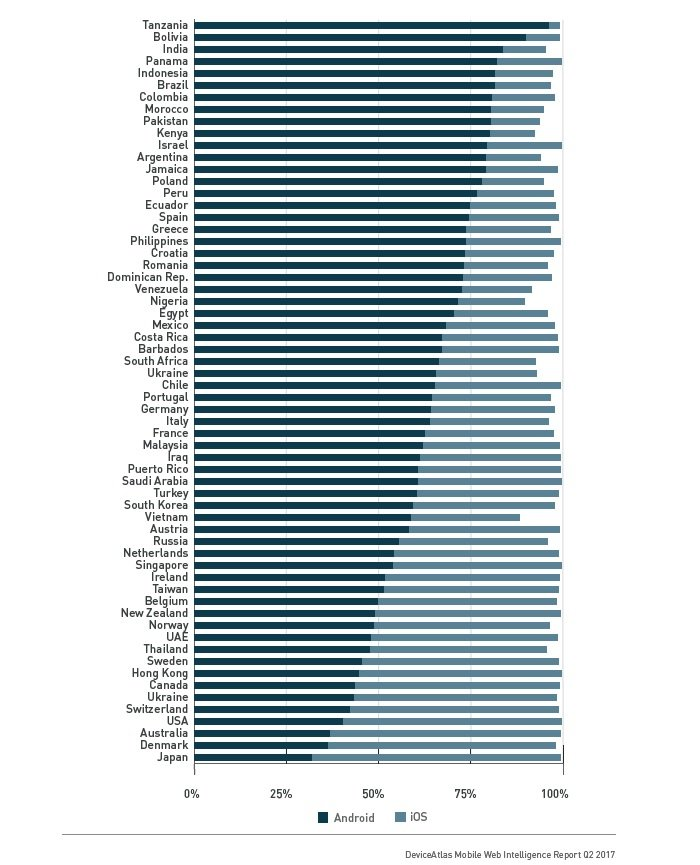
\includegraphics[scale=0.6]{figures/ios_android.jpg}
\caption{\textit{Android} vs \textit{iOS} en diferentes países.\label{fig:and_vs_ios}}
\end{center}
\end{figure}

Como vemos en la figura~\ref{fig:and_vs_ios}, \textit{Android} tiene una mayor aceptación entre el público, sobre todo porque estos móviles tienen precios más asequibles que los que tienen \textit{iOS}. \textit{Android} es utilizado por diversos fabricantes de teléfonos móviles, por esto es que hay mucha competencia y los precios bajan, pero la parte mala de esto es que tenemos un amplio abanico de \textit{Hardware} con diferentes requisitos, complicando la tarea al programador. Los terminales de \textit{Apple} son más caros pero su \textit{Hardware} está especialmente diseñado y optimizado para funcionar de la mano con su propio sistema operativo.

Los terminales móviles poseen una gran cantidad de sensores, entre ellos se encuentra un receptor \textit{GPS}, el cual se puede utilizar para obtener nuestra posición en cualquier punto del globo. Pero esta tecnología tiene un punto débil: los espacios interiores, ya que en ellos la señal no penetra adecuadamente y no puede darnos nuestra ubicación con exactitud. Aquí aparece una nueva necesidad, a la que se ha intentado dar solución en los últimos años de diferentes maneras: con \textit{WiFi}, \textit{Bluetooth}, y otras tecnologías inalámbricas. Pero todavía hay muchas barreras, como la obligación de calibrar el entorno previamente o la necesidad de infraestructura auxiliar como transmisores \textit{Bluetooth} o \textit{WiFi} auxiliares.

En nuestro caso, utilizaremos esta tecnología para la obtención de publicidad basada en la ubicación del cliente dentro de centros comerciales. Y los datos sobre la posición del usuario serán proporcionados por la plataforma \textit{Situm}, que nos da la localización de un usuario en un entorno previamente calibrado con una precisión bastante buena. Gracias a esta aplicación, las tiendas podrán emitir publicidad por un nuevo canal y los consumidores podrán disfrutar de ofertas, descuentos y estar al tanto de productos de su interés que se encuentren en su entorno.


\section{Objetivos}
El objetivo principal de este proyecto es crear una red publicitaria que se distribuirá entre los potenciales clientes según su ubicación en tiempo real. Se utilizarán técnicas de posicionamiento en interiores para solventar las limitaciones de cobertura propias del \textit{GPS}, pero sin dejarlo de lado, de tal manera que la aplicación podrá utilizarse en espacios abiertos y cerrados. Los objetivos principales serán los siguientes:
\begin{itemize}
\item Autenticación de los usuarios y asignación por roles.
\item Publicación de ofertas.
\item Disfrute de dichas ofertas por parte de los clientes.
\end{itemize}

%%
\section{Propuesta}
Proponemos desarrollar una plataforma de publicidad geolocalizada  divida en tres componentes:
\begin{enumerate}
\item \textbf{Sistema de localización de interiores.} Se utilizarán los servicios ofrecidos por la plataforma \textit{Situm}.
\item \textbf{Sistema de almacenamiento en la nube.} Para almacenar toda la información relativa a usuarios, ofertas, tiendas, edificios, roles, permisos e imágenes. Nos hemos decantado por la \textit{API} de \textit{Firebase Google}, que nos ofrece gran cantidad de servicios en la nube, aunque hay otros muchos disponibles. Los servicios de \textit{Firebase} que usaremos en este proyecto serán: base de datos no relacional, \textit{API REST}, \textit{Cloud Functions} y autenticación. 
\item\textbf{ Aplicación móvil \textit{iOS}.} Será la parte de cliente, que se comunicará con los servidores de \textit{Situm} y con \textit{Firebase} a través de su \textit{API REST}. La interfaz y las acciones que podrá llevar a cabo el usuario, dependerán de su rol.
\end{enumerate}

\section{Estructura de la memoria}
En los capítulos siguientes, se profundizará en las múltiples fases del desarrollo de este proyecto. A continuación, un breve resumen del contenido de estos:
\begin{itemize}
\item \textbf{Estado del arte.} Aplicaciones de la localización en interiores en la actualidad.
\item \textbf{Fundamentos teóricos.} Bases teóricas sobre las que se asienta la tecnología de posicionamiento en interiores.
\item \textbf{Fundamentos tecnológicos.} Este capítulo explicará las tecnologías empleadas para el desarrollo de este proyecto en concreto.
\item \textbf{Análisis.} Este capítulo tratará el análisis de requisitos, actores y casos de uso.
\item \textbf{Metodología.} Aquí se explicará la elección de la metodología de desarrollo y su adaptación a este proyecto concreto.
\item \textbf{Gestión de proyecto.} En este capítulo se hablará sobre la planificación de las tareas, estimaciones de costes y valoración de riesgos.
\item \textbf{Arquitectura.} Se expondrá la arquitectura del proyecto, como se estructuraron los diferentes componentes.
\item \textbf{Implementación.} Se tratarán aquí los detalles de la implementación, a partir de la arquitectura comentada en el capítulo anterior.
\item \textbf{Pruebas.} Se hablará sobre las pruebas realizadas a lo largo de la realización del proyecto y al final del mismo.
\item \textbf{Conclusiones.} Como cierre de la memoria, hablaremos sobre las  conclusiones, lecciones aprendidas a lo largo de todo el desarrollo y del trabajo que nos queda por delante en caso de continuar con el proyecto.
\item{}\textbf{Instalación y uso.} En este apéndice, se guiará al usuario a través del proceso de instalación de la aplicación y se le indicará como utilizar las funcionalidades básicas.
\end{itemize}


\chapter{Estado del arte}
Este capítulo hablará sobre los posibles usos de la localización en interiores, pero no sólo orientados al marketing y la publicidad, sino también a muchos otros sectores.

\section{\textit{Senion}}
En esta sección se hablará sobre una compañía llamada \textit{Senion} que ofrece múltiples aplicaciones que funcionan mediante posicionamiento en interiores, entre ellas encontramos varias orientadas a la publicidad y al marketing.

\subsection{Publicidad y marketing en interiores}
Aquí se comentarán algunos ejemplos de aplicaciones reales que han sido desarrolladas basándose en las herramientas ofrecidas por esta compañía:

\paragraph{\textit{Mall of America}.} el centro comercial más grande de Norte América ha instalado un sofisticado sistema de posicionamiento \textit{indoor} con la ayuda de la compañía \textit{Senion}. La tecnología está diseñada para mejorar la experiencia del usuario, dirigiéndolo a las tiendas, restaurantes o lugares de entretenimiento deseado a través de una \textit{app} en sus teléfonos móviles \cite{noauthor_mall_nodate}.
\paragraph{\textit{Dubai Mall}.} el centro comercial más visitado del mundo también tiene un sistema de posicionamiento \textit{indoor} que utiliza las herramienta ofrecidas por \textit{Senion}. Es lógico que un centro comercial de estas dimensiones y con unas 1200 tiendas y 200 restaurantes, necesite un sistema de localización en interiores para que sus visitantes no se pierdan. Como en el caso de uso anterior, también dispone de una \textit{app} propia \cite{noauthor_dubai_nodate}.
\paragraph{\textit{GINZA SIX}.} en este centro comercial de \textit{Tokyo} de 8 plantas, los compradores también pueden orientarse y conocer la ruta más rápida a su destino mediante un sistema de posicionamiento en interiores utilizando una red de \textit{beacons} y una aplicación para sus teléfonos móviles \cite{noauthor_ginza_nodate}.
\paragraph{Centro comercial Parque Arauco.} también tiene su propia aplicación basada en este tecnología \cite{noauthor_parque_nodate}.

\subsection{Eventos}
Otro uso del posicionamiento en interiores, sería el de facilitar los desplazamientos por festivales, eventos y otros lugares a donde la señal \textit{GPS} no puede acceder.

\paragraph{Feria de \textit{eCommerce} en Sao Paolo 2015.} En este evento, se lanzó una aplicación móvil que permitía a los visitantes conocer los \textit{stands} que estaban presentes en la feria y recibir indicaciones para llegar hasta ellos. Incluso los usuarios podían registrarse, crear un perfil y hacer su ubicación visible a otras personas, esto podría ser una posible idea para el futuro: el posicionamiento en interiores orientado a las redes sociales. Pero además, la aplicación también proporcionaba ventajas a los organizadores de la feria y propietarios de stands. Estos podían obtener datos estadísticos sobre los movimientos de los visitantes, como mapas de calor y los puntos en los que más personas suelen pararse \cite{noauthor_feria_2015}.

\subsection{Organización en las empresas}
Muchas empresas realizan estudios sobre el tiempo que pierden sus empleados yendo de un sitio para otro buscando a otro compañero, el cual quizás no se encuentre en su puesto habitual. Una aplicación que ubicase a cada empleado, podría solucionar este problema, produciendo un sustancial ahorro de tiempo para los empleados y de dinero para la empresa.

\paragraph{\textit{Ericsson optimized workplace}.} En las oficinas de \textit{Ericsson} situadas en Estocolmo, las cuales tienen una enorme superficie. La empresa \textit{Senion} en colaboración con \textit{Flowscape} \cite{noauthor_flowscape_nodate}, ha desarrollado una plataforma que incrementa en gran medida la productividad de los empleados. Esta herramienta es muy necesaria en una oficina de 20 pisos distribuidos en 4 edificios y no sólo hace muy sencillo encontrar a personas, sino también lugares o salas \cite{noauthor_ericsson_nodate}.

\section{\textit{Situm}}
En esta sección se hablará sobre la plataforma \textit{Situm}, la cual ha sido elegida para este proyecto y sus casos de éxito \cite{situm_casos_nodate}.

\paragraph{Servicios sanitarios}
Aplicación que mejora la relación entre el ciudadano y el sistema sanitario permitiendo a los pacientes y a los visitantes navegar en el interior de los hospitales a través de sus smartphones, buscar puntos de interés (consultas, salas de espera, tiendas, paradas de transporte…) y obtener rutas guiadas.
La tecnología de \textit{Situm} está presente en docenas de hospitales públicos y privados en España, Turquía y Tailandia, incluyendo algunos de los centros más grandes y complejos de Europa como el hospital Álvaro Cunqueiro, en Vigo, el hospital Lucus Augusti, en Lugo, y el hospital de Mersin \cite{situm_indoor_2018}.

\paragraph{Seguridad}
\textit{Situm} también ofrece una solución de posicionamiento en interiores, identificación y monitorización del personal de seguridad, además de nuevas e innovadores funciones basadas en la localización como alertas de hombre caído, botón de pánico y asignación de tareas geolocalizadas \cite{securitas_seguridad_espana_securitas_2018}.

\paragraph{Centros comerciales}
Esta tecnología puede ser integrada en las aplicaciones de \textit{retailers} para proveer un mejor servicio a sus clientes y para obtener información geoestadística, incrementando de esta forma el \textit{business intelligence} y mejorando el \textit{ROI} mediante el geomarketing.
\textit{Situm} ya está presente un número creciente de centros comerciales en América, Asia y Europa.

\paragraph{Servicios}
Aplicaciones de posicionamiento en interiores que permiten guiar al usuario en edificios públicos multitudinarios como aeropuertos y estaciones de tren/autobús desde su posición hasta los principales puntos de interés (\textit{check-ins}, controles de seguridad, puertas de embarque…), incluidos todos los servicios disponibles en el interior de estos edificios (aseos, tiendas, restaurantes…).
La tecnología de \textit{Situm} está siendo usada en aeropuertos internacionales, mejorando no sólo la experiencia de los viajeros, sino proveyendo también información valiosa que puede ayudar a los gestores de los edificios a monitorizar servicios clave como el personal \textit{PMR} (favoreciendo de esta forma la localización de pasajeros con movilidad reducida) y a incrementar la rentabilidad de sus operaciones no aeronáuticas mediante una mejor explotación de sus áreas comerciales.

\paragraph{Edificios corporativos}
\textit{Situm} ayuda a organizaciones públicas y privadas con sedes grandes y complejas a mejorar la eficiencia de su gestión de personal, al mismo tiempo que facilita el día a día de sus trabajadores y visitas posibilitando que puedan explorar el mapa del edificio, localizar puntos de interés (desde plazas de parking libres a salas de reuniones) y obtener rutas guiadas.
La tecnología de localización en interiores de \textit{Situm} ya está funcionando en varias sedes corporativas de Asia, Europa y Estados Unidos.

\paragraph{Industria 4.0}
\textit{Situm} provee datos en tiempo real de la interacción de activos móviles con otros elementos (como carretillas, \textit{AGVs} y demás vehículos logísticos) en el interior de ambientes industriales, proporcionando información valiosa para la optimización del proceso logístico y del uso de estos vehículos. La tecnología de \textit{Situm} destaca debido a su mínimo tiempo de despliegue, y reduce significativamente los costes de instalación gracias a que puede funcionar con la infraestructura existente.
La versatilidad de \textit{Situm} permite que su sistema pueda ser adaptado en una amplia variedad de aplicaciones para solventar problemas logísticos.
El Grupo \textit{PSA} ha escogido a \textit{Situm} como una de las mejores \textit{startups} a nivel mundial por \textit{Situm Factory Indoor}, una solución que adapta su tecnología para localizar otros elementos que no sean personas y poder hacerlo desde dispositivos dedicados.

\paragraph{Eventos}
\textit{Situm} funciona en grandes infraestructuras que acogen eventos masivos como congresos, espectáculos y encuentros deportivos (en estadios de fútbol y baloncesto). Edificios complejos con muchas señales \textit{WiFi} y \textit{Bluetooth}. Con la tecnología de \textit{Situm}, los organizadores de los eventos obtienen información valiosa que les puede ayudar a monetizar mejor sus espacios, proveyendo al mismo tiempo localización y navegación en interiores a sus visitantes.\\
Su tecnología proporciona servicios en los mayores centros de congresos, como \textit{Fira} de Barcelona (una de las instituciones feriales más importantes de Europa) a través de la solución \textit{Securitas Location} \cite{situm_indoor_2018-1}.
\chapter{Fundamentos teóricos}
En este capítulo, hablaremos sobre las bases teóricas utilizadas para obtener la posición de un teléfono móvil, gracias a la gran cantidad de sensores que tiene. Dividiremos el capítulo en dos secciones: Técnicas y Tecnologías. Gran parte de la información fue obtenida de este artículo \cite{mohamad_yassin_elias_rachid_survey_2015}.

\section{Técnicas de posicionamiento en interiores} \label{tecnicas}
En esta sección hablaremos sobre algunas de las múltiples maneras de calcular la posición de un receptor.

\subsection{Potencia con la que recibimos la señal} \label{rssi}
En inglés, \textit{Received Signal Strength} (\textit{RSS}). Es una de las maneras más simples de localizar en interiores, es la fuerza de la señal recibida en el receptor y se mide normalmente en decibelios de milivatio o en milivatios. Se usa para medir la distancia entre el emisor de la señal y el receptor, cuanto mayor es la potencia recibida, menor es la distancia. No confundir con \textit{Received Signal Strength Indicator} (\textit{RSSI}), este último viene definido por cada fabricante y cada uno le pone los valores que le da la gana, pero básicamente y como su nombre indica, estos hacen referencia a la \textit{RSS}.

\begin{figure}[t]
\centering
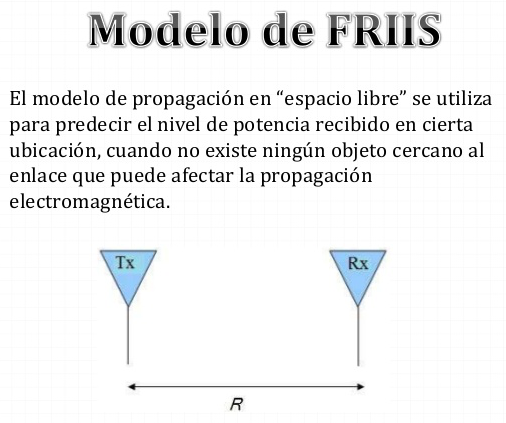
\includegraphics[scale=0.4]{figures/friis.png}
\caption{Propagación de onda electromagnética en espacio libre.\label{fig:friis}}
\end{figure}

Si queremos saber la distancia a la que se encuentra el transmisor observando el \textit{RSSI} del receptor, simplemente deberemos aplicar la siguiente fórmula:
\begin{equation}
RSSI = -10n\log_{10}(d) + A,
\end{equation}
donde \textit{n} es la constante de propagación, \textit{A} es el valor \textit{RSSI} de referencia en dBm (a 1 metro del transmisor) y \textit{d} es la distancia que nos interesa, en metros. Si deseamos calcular \textit{d} en un espacio sin obstáculos también llamado espacio libre (ver figura \ref{fig:friis}), debemos poner ${n = 2}$, cuanto mayor sea este valor, mayores serán las pérdidas de potencia a lo largo del viaje de la señal, en un entorno con obstáculos podríamos poner ${n = 4}$.

Para calcular una posición según este método, habría que tener más de un transmisor (cuantos más mejor) cuya señal llegase hasta receptor. Desde el receptor, conocemos el \textit{RSSI} y por tanto la distancia a la que se encuentra cada transmisor. Ahora si cogemos un papel y dibujamos circunferencias, cada una con centro en un transmisor y con un radio que sería la distancia entre este y el receptor. La posición que buscamos estaría dentro del área de intersección de todas las circunferencias. Un teléfono móvil no tiene que dibujar circunferencias, utilizando fórmulas matemáticas enseguida halla sus coordenadas, pero para saber cuales son, deben conocer previamente las coordenadas de los transmisores, que tomaría como puntos de referencia.

\begin{figure}[tbp]
\centering
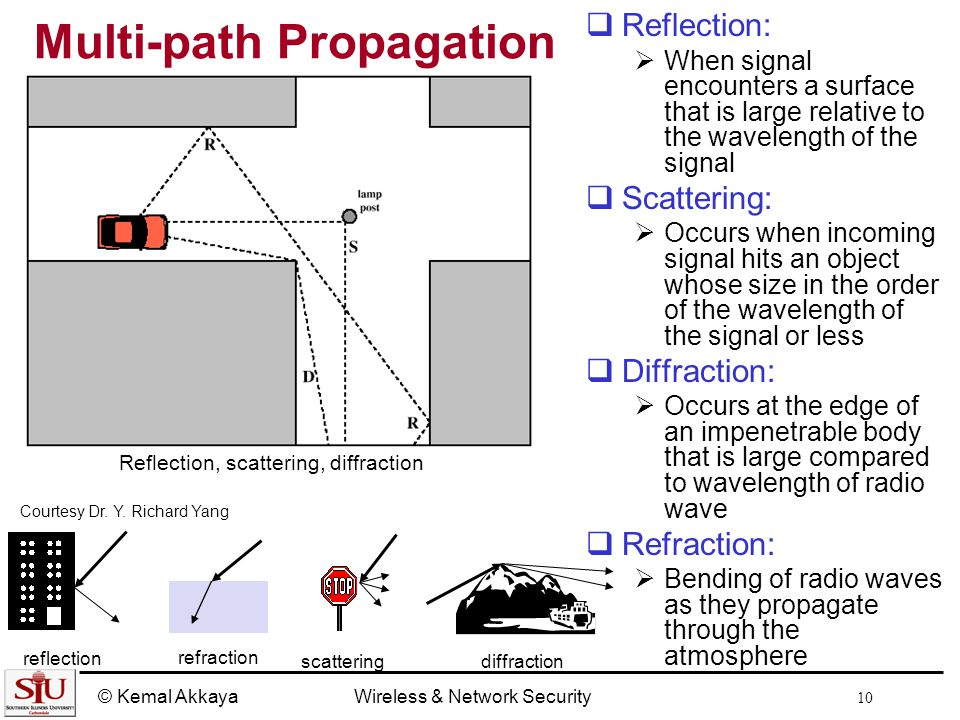
\includegraphics[scale=0.38]{figures/multipath.jpg}
\caption{Fenómeno conocido como \textit{multipath}.\label{fig:multipath}}
\end{figure}

Una limitación de esta técnica de posicionamiento en interiores, es que un área de intersección más grande se traduce en una menor precisión, lo que se suele hacer es tomar como resultado un punto medio. Además surge otro problema, cuando hay obstáculos, en lugar de trazar una línea recta entre transmisor y receptor, la señal va rebotando hasta llegar a su destino, perdiendo intensidad, tardando más y pareciendo así que está más lejos. Esto también contribuye a que la señal realice el viaje por múltiples caminos, llegando varias veces al destino y con valores de \textit{RSSI} diferentes, ver figura~\ref{fig:multipath}.

\subsection{Recolección previa de valores \textit{RSSI} en diversos puntos}
Inicialmente, se recolectan valores \textit{RSSI} en diversos puntos, podríamos llamar a esto, fase de calibración. Una vez tomadas estas medidas a lo largo de toda la superficie deseada, podemos empezar a movernos con nuestro receptor. Este irá comparando los valores \textit{RSSI} que obtiene a cada instante, con los que fueron recolectados durante la fase inicial, obteniendo así su posición.

La precisión de este sistema depende de la cantidad de medidas que tomemos en la fase inicial, es tentador pensar que a más cantidad, mejor funcionamiento, pero hay que tener en consideración otro parámetro: la distancia entre puntos. Cuanto menor sea esta distancia, más fácil será confundir una posición con las colindantes, bajando así la precisión del sistema. Otro punto débil de este sistema es la sensibilidad a los cambios del entorno, cuando lo calibramos se dan unas condiciones (cantidad de personas, humedad, posición de los transmisores, etcétera) que puede que no se conserven cuando el sistema esté en funcionamiento. Por ello es importante, que la calibración se realice bajo unas condiciones que se acerquen lo máximo posible a las que encontraríamos en una situación normal y que los transmisores se encuentren en la misma posición siempre.


\section{Tecnologías utilizadas para el posicionamiento en interiores}
En esta sección hablaremos sobre algunas tecnologías que nos permiten llevar a cabo las técnicas comentadas anteriormente para obtener la posición de un receptor en un espacio cerrado.

\subsection{\textit{WiFi}}
Las especificaciones del estándar \textit{IEEE 802.11}, proporcionan la base para los productos con redes inalámbricas que hacen uso de la marca \textit{WiFi}. Su principal cometido es facilitar la comunicación y conexión a Internet, es por este motivo, que podemos encontrar esta tecnología en casi todos los dispositivos portátiles que se fabrican en la actualidad. Está tan extendido, que es sumamente difícil encontrar un lugar en cualquier ciudad o edificio en el cual nuestro teléfono no sea capaz de detectar ningún punto de acceso inalámbrico. Esto lo convierte en un pilar fundamental para el posicionamiento en interiores, pero también es su principal debilidad: el hecho de que sea un canal muy usado ya para las comunicaciones y lleno de interferencias, puede afectar en gran manera a la precisión de la localización.

\subsection{Bluetooth}
En el estándar \textit{IEEE 802.15.1} están definidas las especificaciones físicas y de control de acceso al medio que conforman las bases de la tecnología inalámbrica \textit{Bluetooth}. En su última versión \textit{Bluetooth Low Energy} o \textit{BLE}, se ha mejorado la eficiencia energética a costa de una reducción notable de las velocidades de transferencia que se alcanzaban en \textit{Bluetooth Classic}, el \textit{Bluetooth} que todos hemos usado alguna vez para pasarnos algún fichero cuando los teléfonos todavía no tenían acceso a Internet.

El \textit{BLE} está jugando un papel muy importante en el posicionamiento en interiores debido a su bajo consumo, con una simple pila de botón podemos alimentar un pequeño transmisor que puede pasarse años transmitiendo balizas periódicamente. Otro factor que está consolidando esta tecnología es la inclusión de la misma en casi todos (sino todos) los dispositivos con \textit{Bluetooth}, y es que no hay que confundir \textit{Bluetooth Classic} con \textit{BLE}: son protocolos diferentes, transmiten los datos de manera diferente y lo más importante, son incompatibles,ver tabla~\ref{tab:bluetooth_ble}. Un aparato que sólo tiene \textit{Bluetooth Classic} nunca podrá comunicarse ni detectar a otro que sólo tenga \textit{BLE}.

Conviene hablar un poco más sobre esta tecnología porque cada vez está más presente en nuestro día a día y es, junto con el \textit{WiFi}, uno de los pilares fundamentales del posicionamiento en interiores.

\begin{table}[tbp]
\begin{center}
\small
\begin{tabular}{|l|c|c|}
\hline 
Especificación técnica & \textit{Bluetooth Classic} & \textit{BLE}  \\
\hline 
\hline
Frecuencia & 2.4GHz & 2.4GHz \\
\hline
Distancia & 10m & 10m \\
\hline
\textit{Data rate} & 0.7-2.1Mbit/s & 0.2Mbit/s \\
\hline
Transmisión de voz & Sí & No \\ 
\hline
Consumo & 1 (referencia) & 0.01 a 0.5 (depende del uso) \\
\hline
Consumo corriente pico & 30mA & 15mA \\
\hline
\end{tabular}
\caption{Bluetooth Classic vs BLE.\label{tab:bluetooth_ble}}
\end{center}
\end{table}

\subsubsection{Utilización de dispositivos \textit{BLE} para transmitir información}
Un dispositivo puede tomar dos roles en esta comunicación, ver figura~\ref{fig:connect-ble}:
\begin{itemize}
\item \textbf{Maestro.} Escanea su entorno en busca de periféricos con los que establecer una conexión, la cual siempre será iniciada por el maestro. Podrá estar conectado a varios periféricos simultáneamente y podrá desconectarse de cada uno de ellos cuando quiera.
\item \textbf{Periférico.} Se anuncia mediante balizas para que los maestros lo detecten y se puedan conectar a él si así lo desean, una vez iniciada la conexión, dejan de emitirse las balizas, ya que un periférico sólo puede estar conectado a un maestro simultáneamente.
\end{itemize}

\begin{figure}[tbp]
\centering
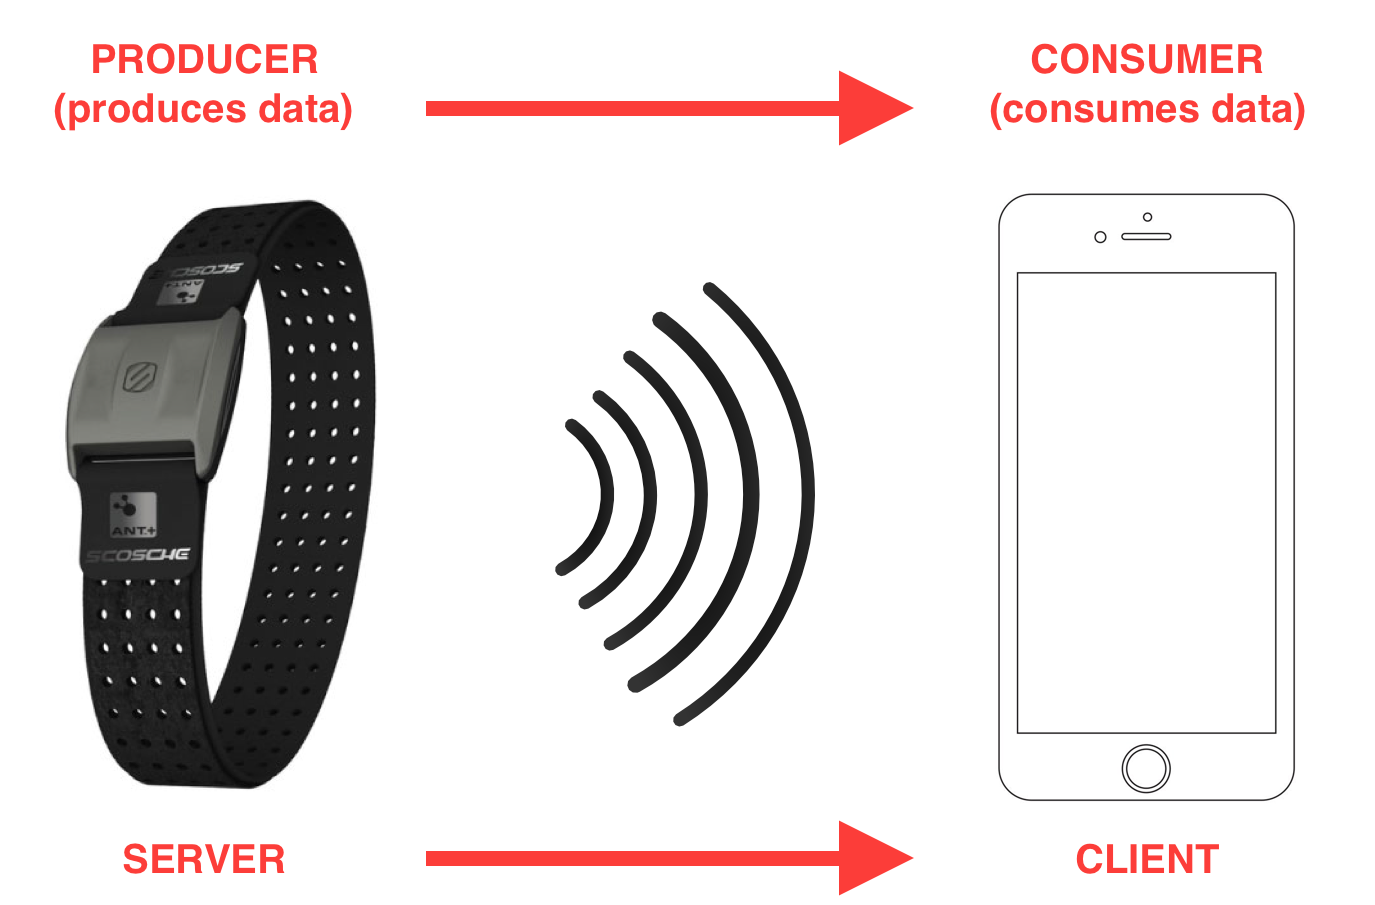
\includegraphics[scale=0.15]{figures/communication-ble.png}
\caption{Un \textit{smartwatch} se conecta mediante \textit{BLE} al \textit{smartphone} con el que quiere comunicarse.\label{fig:communication-ble}}
\end{figure}

Un ejemplo de esta funcionalidad sería un teléfono móvil (maestro) y un reloj inteligente (periférico) que recibe y muestra las alertas del teléfono y que además nos mide las pulsaciones y las envía al teléfono para llevar a cabo un seguimiento. El teléfono podría estar conectado también a otros periféricos como por ejemplo un báscula o un sensor de temperatura, pero el reloj inteligente ya no podrá anunciarse, ni mucho menos conectarse, con otro dispositivo hasta que el maestro se desconecte de él, ver figura~\ref{fig:communication-ble}. La comunicación puede realizarse en ambos sentidos (teléfono ${\leftrightarrow}$ reloj), mediante un protocolo con unas normas fijas para todos los dispositivos, pero que permite adaptarse a las necesidades de cada fabricante.

En \textit{BLE} hay definidos una serie de servicios: pulsaciones, alertas \textit{SMS}, llamadas y un largo etcétera . Cada uno de ellos tiene asociados unos identificadores estándar, para que cualquiera que los analice sepa como comunicarse con ellos \cite{noauthor_ble_nodate}. Esto facilitaría en gran medida la labor de un desarrollador de aplicaciones móviles, por ejemplo, si quisiera desarrollar una aplicación diferente a la que proporciona el fabricante de un periférico. Pero quizás al fabricante no le interesa que cualquiera pueda saber como funciona su dispositivo, los motivos pueden ser varios: privacidad del usuario, evitar \textit{hackeos}, o simplemente mantener el monopolio de su aplicación y que nadie desarrolle otra que le haga competencia \cite{andrey_nikishaev_how_nodate}.

Lo que hará entonces, será crear sus propios servicios con identificadores que sólo él comprende y, como la comunicación en \textit{BLE} se realiza enviando pequeños paquetes de alrededor de 20 bytes cuyo contenido puede encriptarse por el periférico y desencriptarse por el maestro, o viceversa, muy fácilmente; dificultará en gran medida que alguien ajeno a la empresa comprenda que es lo que está pasando ahí.

Es decir, \textit{BLE} es una infraestructura de comunicación inalámbrica que nos permite diseñar nuestros propios protocolos internos.

\begin{figure}[t]
\centering
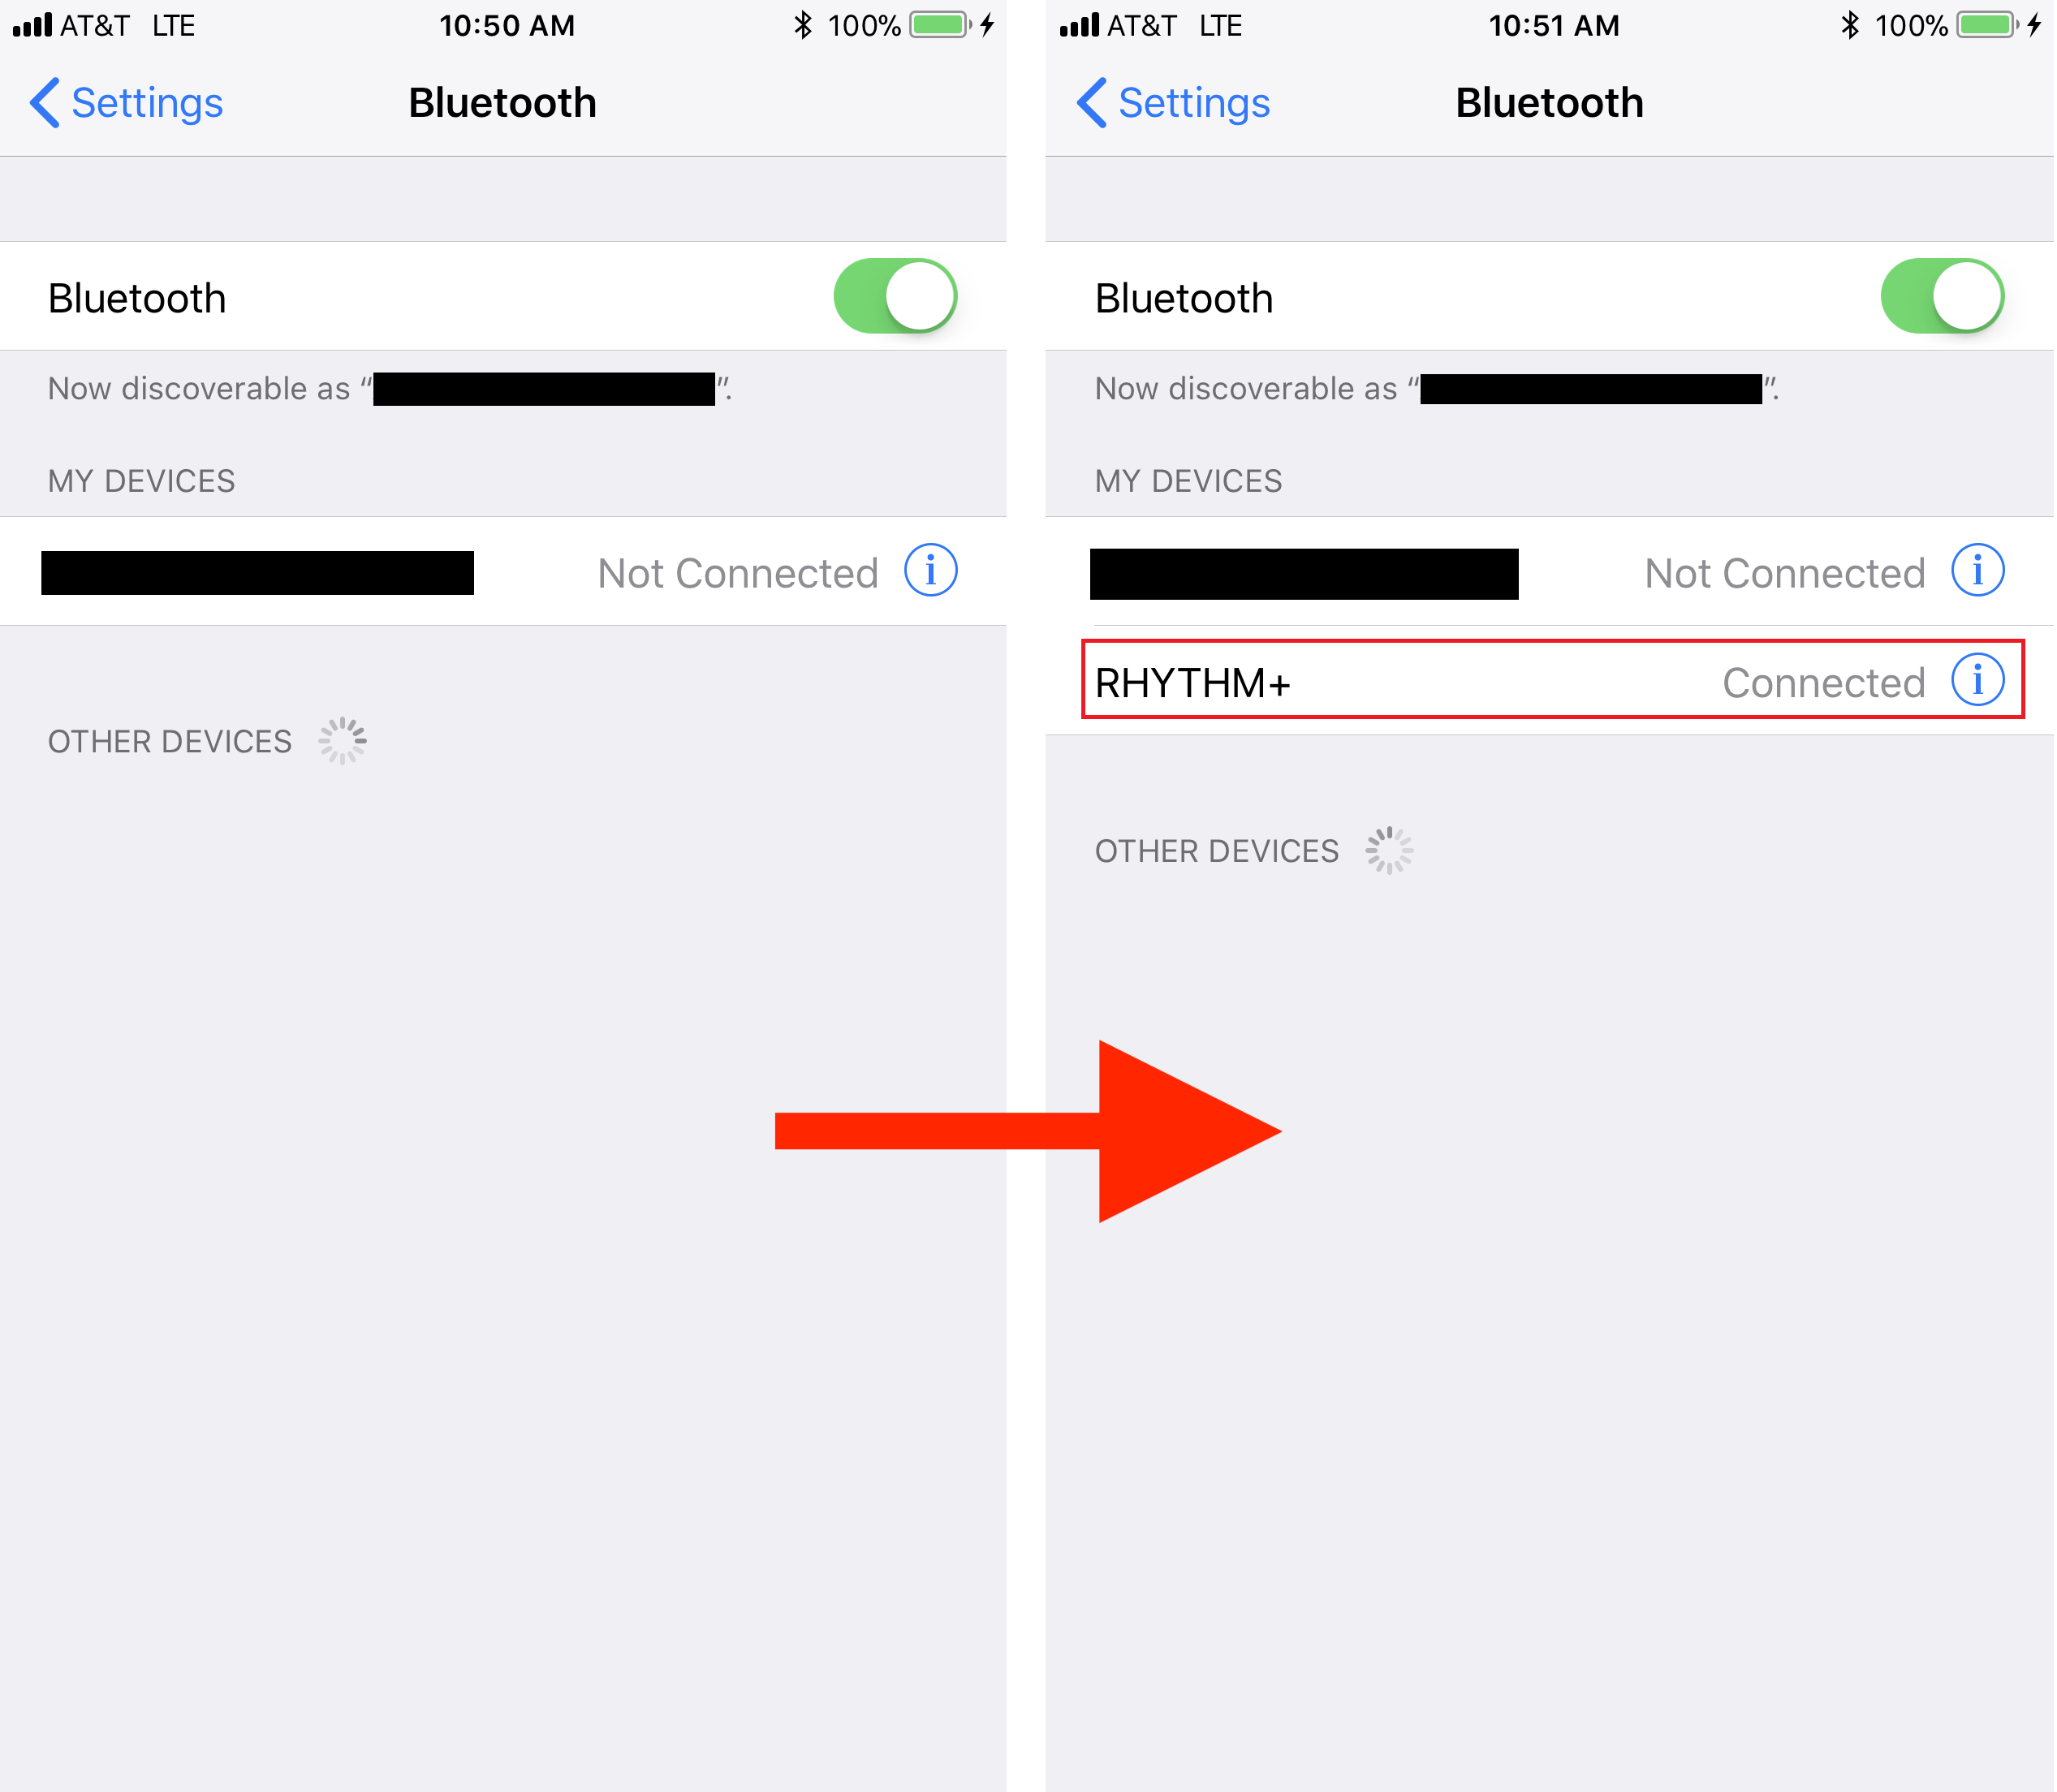
\includegraphics[scale=0.1]{figures/connect-ble.png}
\caption{Se produce una conexión entre maestro y periférico}
\label{fig:connect-ble}
\end{figure}

\subsubsection{Utilización de dispositivos \textit{BLE} como baliza}
Esta funcionalidad es la que más relevancia tiene para este proyecto, pero era necesario que el lector conociese la relación entre maestros y periféricos; y que el \textit{BLE} también puede utilizarse para transmitir pequeñas cantidades de información, para así comprender la diferencia entre un \textit{Smartwatch} y un \textit{Beacon}, que es lo que vamos a explicar ahora.

\begin{figure}[tbp]
\centering
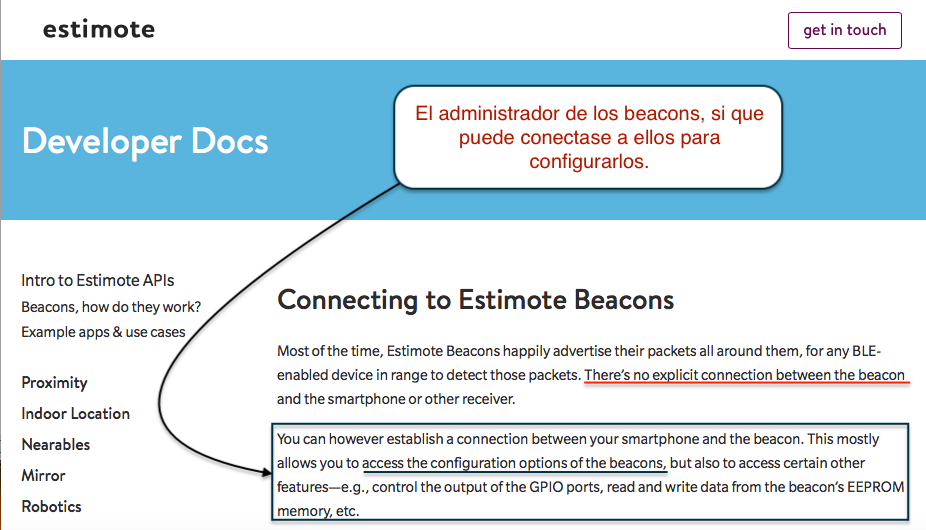
\includegraphics[scale=0.4]{figures/estimote.png}
\caption{Nos podemos conectar a un \textit{Beacon} para configurarlo, pero sólo si tenemos permisos para ello.\label{fig:estimote}}
\end{figure}

Antes vimos que un periférico dejaba de transmitir balizas cuando se conectaba a un maestro, pero no nos interesa que esto pase si lo que queremos es que este dispositivo se siga anunciando para poder utilizarlo como transmisor en un sistema de posicionamiento en interiores. Para lograr este objetivo, lo único que tenemos que hacer es impedir que los maestros puedan conectarse a ese periférico, de esa manera tendremos dispositivos que se estarán anunciando de manera continua e ininterrumpida \ref{fig:estimote}.

Esta es la principal característica de un \textit{Beacon}: es un dispositivo que puede ser detectable por nuestros teléfonos móviles pero al que nunca podrán conectarse. Además la comunicación no es bidireccional como en el caso anterior, nuestro teléfono no enviará ningún dato, solamente podrá leer las balizas emitidas. Las cuales no tendrán un destinatario concreto, sino que cualquier maestro \textit{BLE} que se encuentre en su radio de acción podría recibirlo.

La señal se recibe con un \textit{RSSI} determinado, de manera que mediante triangulación y las técnicas anteriormente comentadas en la sección~\ref{tecnicas}, podremos conocer nuestra posición. Pero no sólo eso, esta señal también transmite información que podríamos leer y que una aplicación podría interpretar para llevar a cabo una acción cuando nos acercásemos a un punto de interés, por ejemplo, hacer saltar una notificación,ver figura \ref{fig:proximity-beacon}.

\begin{figure}[tbp]
\centering
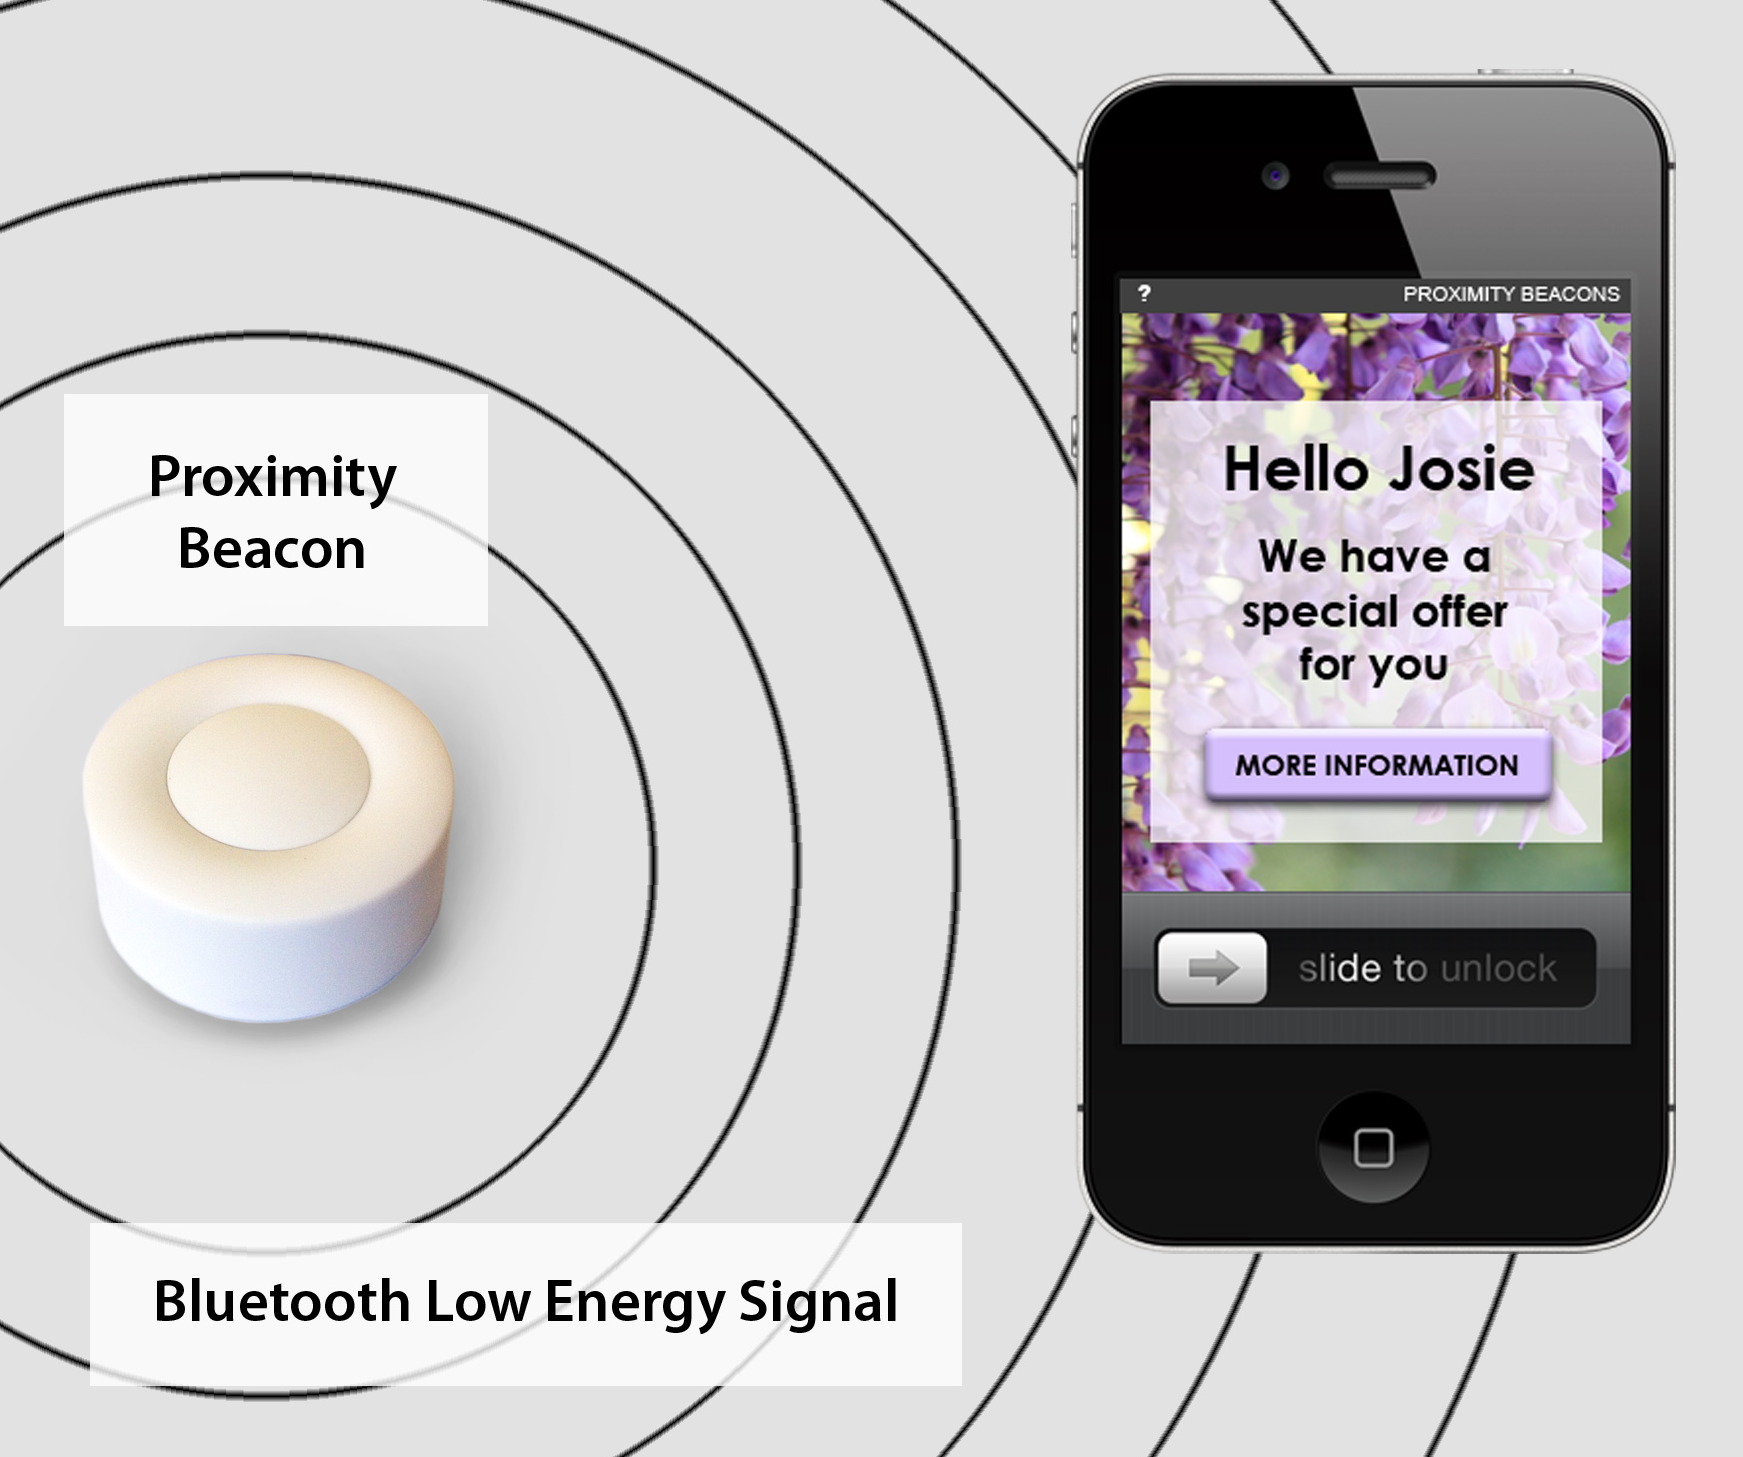
\includegraphics[scale=0.2]{figures/proximity-beacon.png}
\caption{Según el identificador del \textit{Beacon}, se lanza la notificación correspondiente.\label{fig:proximity-beacon}}
\end{figure}

Y es que la intención inicial de las balizas \textit{BLE} no era el posicionamiento en interiores, sino los servicios basados en proximidad. Cada dispositivo tiene un identificador y esto facilita a una aplicación propietaria conocer si el usuario se está acercando a un \textit{Beacon} y saber más o menos a qué distancia se encuentra gracias a la intensidad de la señal. Esto sería de utilidad si no queremos saber donde se encuentra el usuario en cada momento, si lo único que nos interesa es la distancia a la que se encuentra de la baliza. Por ejemplo, si somos una tienda pequeña a lo mejor sólo nos importa que el usuario reciba una notificación al acercarse al comercio. En cambio, si somos un gran supermercado quizás queramos saber donde está el usuario en todo momento. Para comprender los patrones que sigue al moverse por los pasillos, saber en que productos se para más la gente, etcétera (ver figura~\ref{fig:heat-map}). Pero sobre todo, para no tener que poner un \textit{Beacon} en cada punto de interés, ya que con tres dispositivos podríamos triangular al usuario en todo el área que alcanzasen sus señales.

\begin{figure}[tbp]
\centering
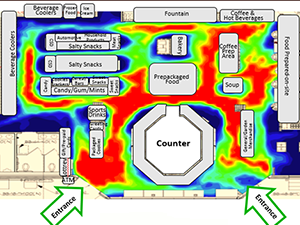
\includegraphics[scale=1]{figures/heat-map.png}
\caption{Mapa de calor creado a partir de los datos de posición de los clientes de un centro comercial.\label{fig:heat-map}}
\end{figure}
\chapter{Fundamentos tecnológicos}
En este capítulo, hablaremos sobre las herramientas escogidas para llevar a cabo el proyecto y el motivo por el que fueron seleccionadas.
En primer lugar comentaremos los servicios de \textit{Backend}, a continuación el servidor de localización en interiores y después las herramientas empleadas durante el desarrollo, especialmente de la aplicación \textit{iOS}. Finalizaremos con las herramientas de gestión del proyecto y de la documentación.

\section{\textit{Backend}}
En esta sección hablaremos del motivo por el que se optó por los servicios ofrecidos por \textit{Firebase}.

\subsection{Estudio alternativas y selección} 
\textit{Firebase} \cite{google_firebase_nodate} es una plataforma de \textit{Google} que nos ofrece una gran cantidad de servicios para desarrollar aplicaciones móviles, de los cuales hemos utilizado el servicio de autenticación, el de base de datos \textit{online} en tiempo real, el de ejecución de código propio y el de \textit{API REST}.

Se decidió utilizar \textit{Firebase} en lugar de crear un servicio propio, por la comodidad que ofrece esta plataforma al tener todos los servicios necesarios (figura~\ref{fig:firebase-services}), siendo el objetivo del proyecto una aplicación móvil y no un servidor web.

\begin{figure}[tbp]
\begin{center}
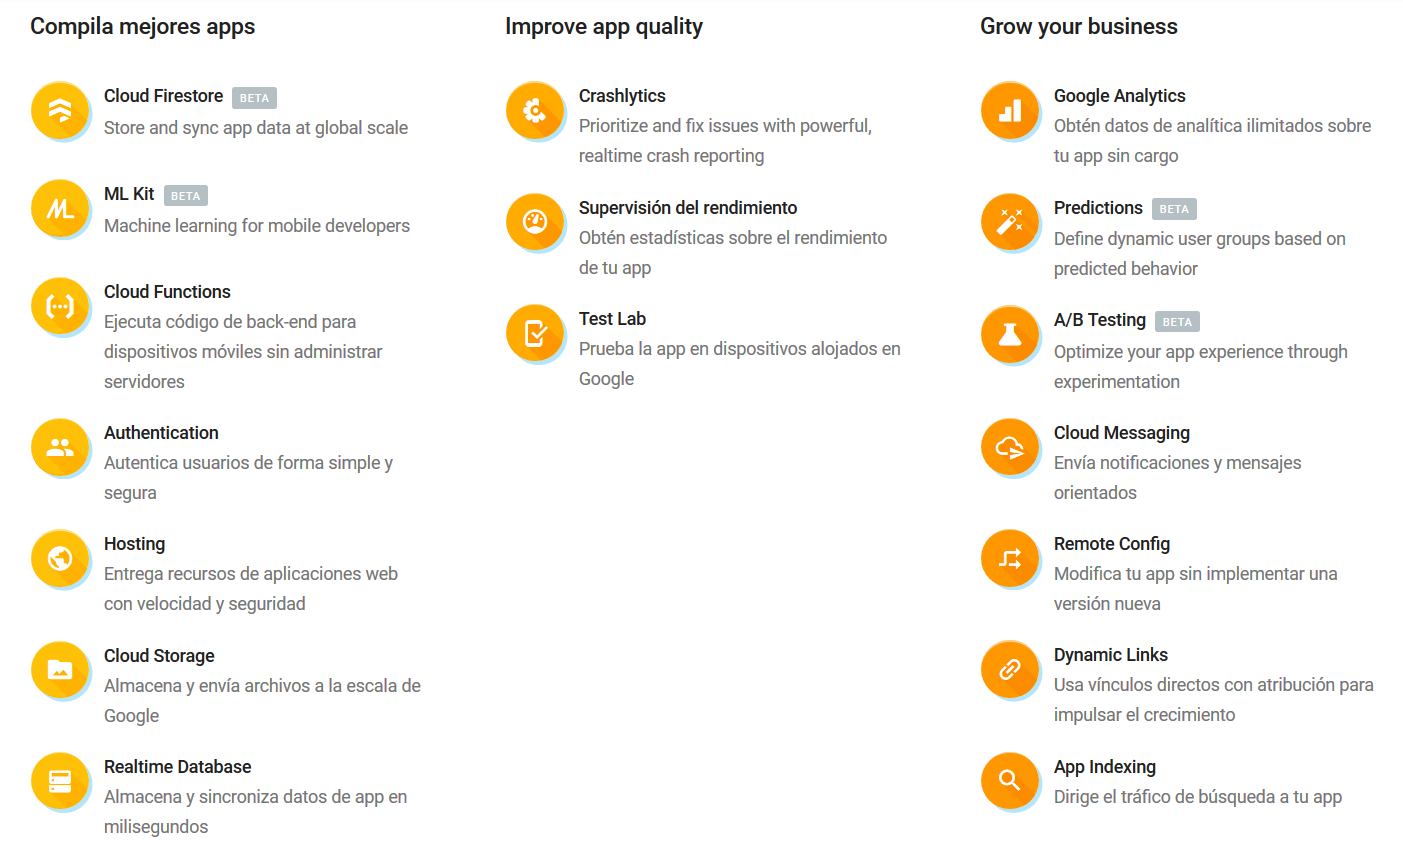
\includegraphics[scale=0.5]{figures/firebase.png}
\caption{Listado de servicios ofrecidos por \textit{Firebase}.\label{fig:firebase-services}}
\end{center}
\end{figure}

\subsection{Autenticación}
\textit{Firebase Authentication} \cite{google_firebase_nodate-1} busca facilitar la creación de sistemas de autenticación seguros, a la vez que mejora la experiencia de incorporación y acceso para los usuarios finales. Proporciona una solución de identidad de extremo a extremo, compatible con cuentas de correo electrónico y contraseñas, autenticación telefónica, \textit{Google}, \textit{Twitter}, \textit{Facebook}, acceso a través de \textit{GitHub} y más (ver subfigura~\ref{fig:auth_methods}).

Hay una gran cantidad de tutoriales \cite{firebase_tutorial_2016} para incorporar este sistema de autenticación a una aplicación \textit{iOS}, incluso hay vídeos oficiales de \textit{Google}. Aunque permite autenticarse de muchas maneras, en este proyecto sólo se contempla la autenticación mediante cuenta de \textit{Google}, no se consideró importante emplear tiempo en añadir otros métodos de inicio de sesión.

\subsection{Base de datos online en tiempo real}
Este servicio de \textit{Firebase} \cite{google_firebase_nodate-2} es uno de los más completos, ofreciendo un gran número de funcionalidades.
\paragraph{Sincronización en tiempo real para datos \textit{JSON}.} \textit{Firebase Realtime Database} es una base de datos \textit{NoSQL} alojada en la nube que te permite almacenar y sincronizar datos entre tus usuarios en tiempo real. Si accedemos a la consola de \textit{Firebase}, que es una página web desde la cual el administrador puede gestionar todos los servicios que tenga en su cuenta. Podemos ver la estructura de la base de datos (ver subfigura~\ref{fig:json}) y exportarla a un fichero \textit{JSON} o importarla de un fichero \textit{JSON}. Esto permite modificar la base de datos a nuestro gusto con un simple editor de texto.

\begin{figure}[tbp]
\begin{center}
\subfigure{
\includegraphics[height=9cm]{figures/fire_auth.png} \label{fig:auth_methods}}
\hspace{10ex}
\subfigure{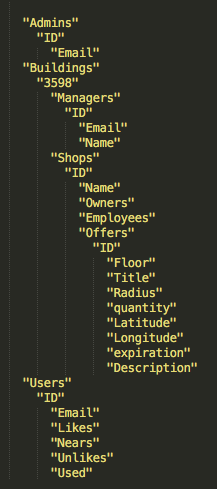
\includegraphics[height=9cm]{figures/json.png} \label{fig:json}}
\caption{\textit{Firebase}: (a) Métodos de autenticación permitidos y (b) almacenamiento de datos.}
\end{center}
\end{figure}

\paragraph{Colabora entre dispositivos con facilidad.} La sincronización en tiempo real permite que los usuarios accedan a sus datos desde cualquier dispositivo, web o móvil, y los ayuda a trabajar en conjunto.

\paragraph{Crea apps sin servidores.} \textit{Realtime Database} se incluye en los \textit{SDK} para dispositivos móviles y web, de manera que puedas crear apps sin la necesidad de usar servidores. También puedes ejecutar un código de \textit{Backend} que responda a los eventos que se activan con tu base de datos a través de \textit{Cloud Functions} \cite{google_firebase_nodate-3} para \textit{Firebase}.

\paragraph{Optimizada para el uso sin conexión.} Cuando los usuarios se desconectan, los \textit{SDK} de \textit{Realtime Database} usan la caché local del dispositivo para publicar y almacenar cambios. Cuando el dispositivo se conecta, los datos locales se sincronizan de manera automática.

\paragraph{Seguridad sólida basada en usuarios.} \textit{Realtime Database} se integra con \textit{Firebase Authentication} para brindar autenticación intuitiva y sencilla para los programadores. Se puede usar su modelo de seguridad declarativo para permitir el acceso según la identidad de los usuarios o con patrones que coinciden con tus datos.

\subsection{Ejecución de código: \textit{Cloud Functions}\label{sec:cloud_functions}}
Determinadas tareas serían imposibles de realizar únicamente mediante peticiones a la base de datos desde el cliente. Por ello, \textit{Firebase} ofrece la posibilidad de subir a su plataforma no sólo datos, sino también funciones \cite{noauthor_cloud_nodate}. Esta es una de las últimas funcionalidades que se han añadido a \textit{Firebase} y todavía se encuentra en estado beta, pero ya se dispone de una gran comunidad de usuarios que la utiliza, así como mucha información en Internet, guías de uso y ejemplos \cite{noauthor_cloud_nodate-1}.

El lenguaje que se utiliza es \textit{JavaScript} aunque también se nos da la posibilidad de escribir nuestras funciones en \textit{TypeScript}. Además disponemos de una amplia documentación para iniciarnos en el desarrollo de \textit{Cloud Functions}, como es habitual en todos los productos que ofrece \textit{Firebase} \cite{noauthor_documentacion_nodate}. Hay varios tipos de funciones que se pueden subir a la plataforma para interactuar con nuestra base de datos, pero sólo hemos utilizado dos: activadas por una petición HTTP o por un cambio en la base de datos.

\paragraph{Funciones activadas por una petición \textit{HTTP}.} Cada una de ellas tiene asociada una \textit{URL}, a la cual debemos realizar una petición cualquiera (\textit{GET}, \textit{HEAD}, \textit{POST}, etc.) si queremos que se ejecute. Desde estas funciones podemos leer y modificar nodos de la base de datos. Son muy útiles si lo que queremos es realizar acciones periódicas en la base de datos, en nuestro caso, recorrer la base de datos para eliminar aquellas ofertas que hayan caducado \cite{noauthor_http_nodate}.

\paragraph{Funciones activadas por un cambio en la base de datos.} Estas funciones no se pueden activar mediante una petición \textit{HTTP} como las anteriores, en este caso, será una modificación de la base de datos la que provocará que se ejecuten. En lugar de asociarles una \textit{URL}, lo que debemos hacer es asociar cada función a un nodo de la base de datos e indicarle ante que cambio en el mismo deberá ejecutarse \cite{noauthor_realtime_nodate}.

\begin{itemize}
\item[-] \textbf{\textit{onWrite}.} Tras la modificación, creación o eliminación de un dato.
\item[-]\textbf{\textit{onChange}.} Tras la modificación de un dato.
\item[-]\textbf{\textit{onDelete}.} Tras la eliminación de un dato.
\item[-]\textbf{\textit{onCreate}.} Tras la creación de un nuevo dato.
\end{itemize}

En este proyecto, se utilizan estas funciones para eliminar una oferta cuando se han agotado las existencias: cada vez que alguien la canjea, se escribe este escaneo en la oferta, lo cual es detectado por la función que resta uno al número de ofertas disponibles y si llega a cero, la borra de la base de datos.


\subsubsection{Otras consideraciones sobre las \textit{Cloud Functions}}
Un inconveniente de esta herramienta, es que cada vez que se realiza un cambio en una función hay que subirla de nuevo a \textit{Firebase} para ver si esto funciona. Cada una de estas operaciones puede llegar a tardar varios minutos, así que para usuarios no muy experimentados con \textit{Firebase} y \textit{JavaScript}, es recomendable crear un entorno local en el que probar que el código funciona antes de subirlo para no perder mucho tiempo \cite{noauthor_cloud_nodate}.
Además es difícil \textit{debuguear} estos programas, una opción es imprimir \textit{logs}, los cuales se mostrarán en la herramienta web de \textit{Cloud Functions} (subfigura~\ref{fig:logs}). 
También hay la posibilidad de mostrar las funciones que están corriendo en ese momento (subfigura~\ref{fig:functions}).
O de ver las estadísticas sobre las invocaciones que se han llevado a cabo (subfigura~\ref{fig:invocations}).

\begin{figure}[tbp]
\centering
\subfigure{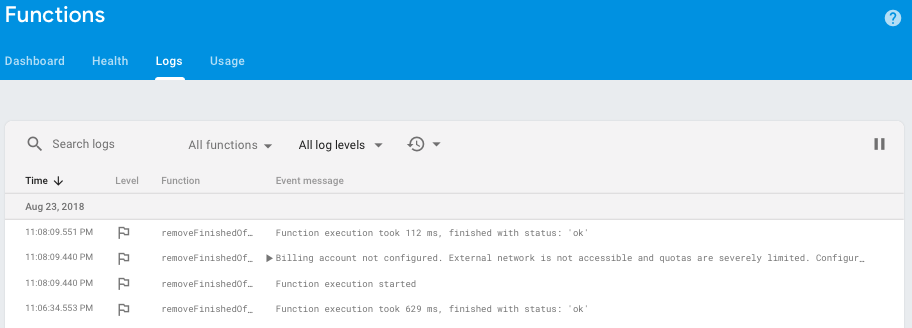
\includegraphics[width=0.9\textwidth]{figures/logs.png}\label{fig:logs}}
\subfigure{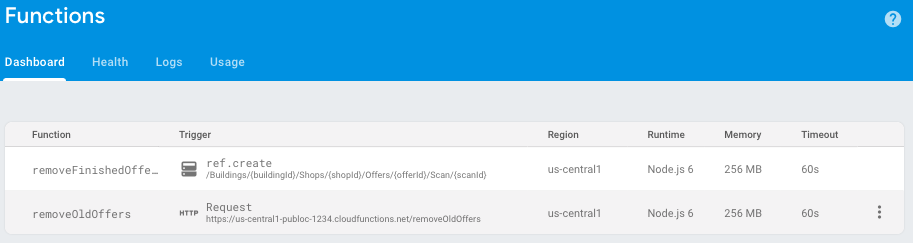
\includegraphics[width=0.9\textwidth]{figures/functions.png}\label{fig:functions}}
\subfigure{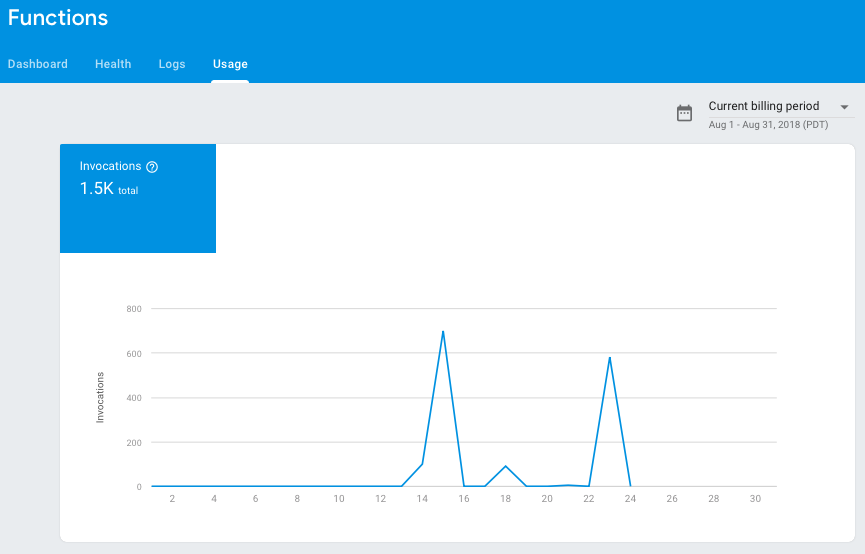
\includegraphics[width=0.9\textwidth]{figures/invocations.png}\label{fig:invocations}}
\caption{\textit{Cloud Functions console}: (a) \textit{Logs} de la ejecución de las diferentes funciones, (b) funciones en ejecución y (c) estadísticas sobre invocaciones de \textit{Cloud Functions}.}
\end{figure}

\subsubsection{Riesgos de las \textit{Cloud Functions}}
Una situación a evitar utilizando \textit{Cloud Functions}, es la recursividad. Una función que se lanza tras una escritura en un nodo de la base de datos puede escribir en ese mismo nodo, si esto sucede se producirá un bucle de escrituras que sólo parará si detenemos la ejecución de la función.

Si nos damos cuenta tarde corremos el riesgo de agotar el cupo de escrituras que nos ofrece \textit{Firebase} con el plan que tengamos contratado y si pagamos bajo demanda podemos llegar a perder bastante dinero si no descubrimos el fallo rápidamente.

\subsection{Comunicaciones en tiempo real: \textit{API REST}}
Se puede acceder a la base de datos desde el código directamente, gracias a las librerías de \textit{Firebase} que debemos importar en el proyecto. Tanto con \textit{Swift} \cite{firebase_firebasedatabase_2018} como con \textit{Objective-C} \cite{firebase_firebasedatabase_2018-1}. Pero en este proyecto se decidió utilizar el \textit{API REST}, debido a la extensa documentación \cite{firebase_firebase_2018} que podemos encontrar en la página oficial, además de que podemos probar las peticiones con más facilidad gracias a herramientas como \textit{Postman}.

\begin{figure}[tbp]
\begin{center}
\subfigure{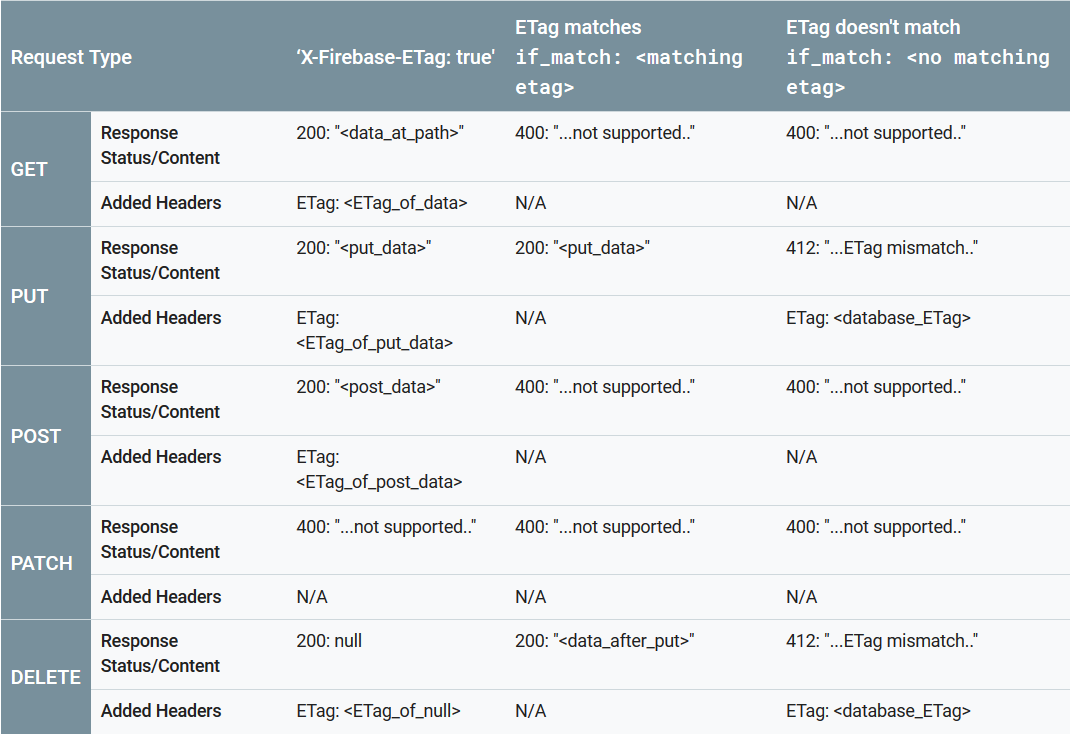
\includegraphics[width=0.9\textwidth]{figures/api_rest.png}}
\subfigure{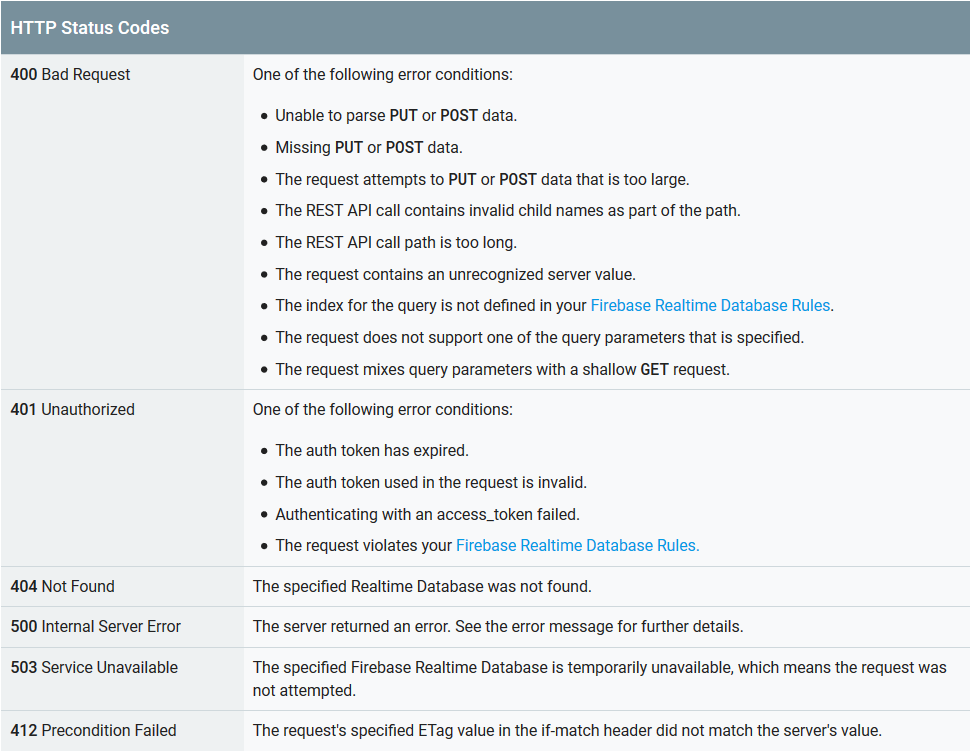
\includegraphics[width=0.9\textwidth]{figures/errors_rest.png}}
\caption{Peticiones \textit{API REST Firebase} y posibles código de errores.}
\end{center}
\end{figure}

Tiene peticiones básicas que permiten variaciones que las hacen más complejas: se puede añadir \textit{tokens} de autenticación en la \textit{URL}, se pueden descargar ficheros, obtener datos ordenados \cite{firebase_firebase_2018-1} o filtrados \cite{firebase_firebase_2018-2}, hacer \textit{streaming} de un valor de la base de datos para tener siempre su valor actualizado, etcétera.

\subsubsection{\textit{Streaming} mediante \textit{API REST}}
Para realizar \textit{streaming} de un nodo a través de la \textit{API REST}, lo que debemos hacer es enviar la cabecera \textit{\textbf{``Accept''}} de la petición con valor \textit{\textbf{``text/event-stream''}}. Esto es posible gracias a que \textit{Firebase} soporta el protocolo \textit{EventSource / Server-Sent Events} \cite{noauthor_eventsource_nodate}.

\section{Servidor localización en interiores \textit{Situm}}
El \textit{SDK} de \textit{Situm} nos da nuestra ubicación en espacios cerrados sin necesidad de añadir infraestructura. Al crearnos una cuenta en la plataforma, podemos empezar a subir mapas de nuestros edificios y calibrarlos.

\subsection{\textit{SDK}}
Es la librería que necesitamos para interactuar con la plataforma \textit{Situm} desde nuestra aplicación móvil. De esta manera, les transmitiremos la información recogida por los sensores de nuestro teléfono y nos será devuelta nuestra posición.

Esta librería también nos permite descargarnos los mapas y toda la información sobre los edificios. Actualmente, hay disponible \textit{SDK} para \textit{iOS} \cite{situm_situm_nodate}, \textit{Android} \cite{situm_situm_nodate-2} y \textit{Cordova} \cite{situm_situm_nodate-1}. Además de un \textit{API REST} \cite{situm_situm_nodate-3}.

\subsection{\textit{Dashboard}}
Mediante esta herramienta web, se pueden crear y editar edificios (subfigura~\ref{fig:mapa_situm_fic}), gestionar calibraciones, descargarnos sesiones de uso y más, ver subfigura~\ref{fig:funcionalidades_situm}.

\begin{figure}[t]
\centering
\subfigure{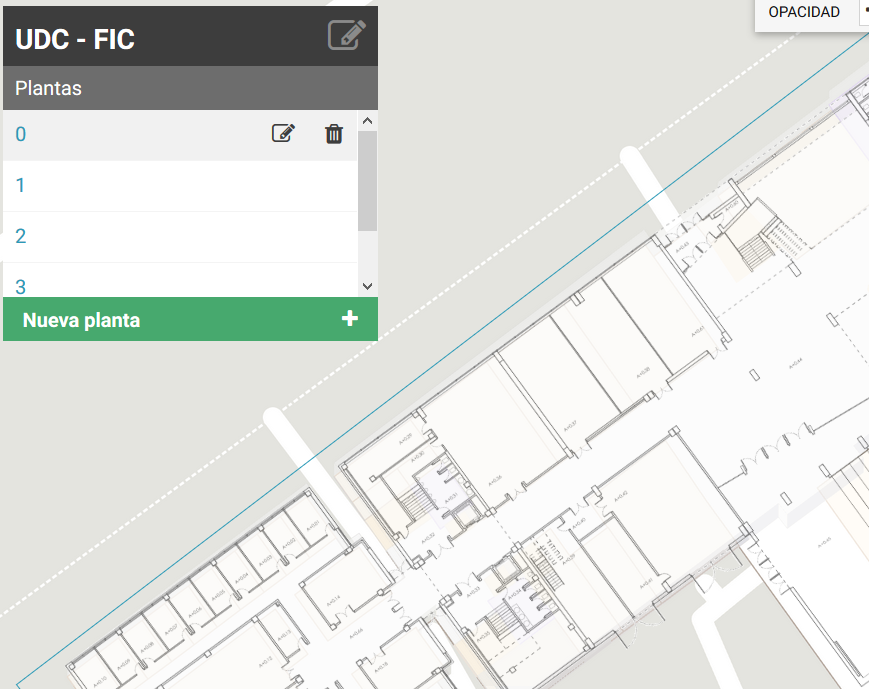
\includegraphics[width=0.4\textwidth]{figures/mapa_situm_fic.png}\label{fig:mapa_situm_fic}}
\subfigure{
\includegraphics[scale=0.5]{figures/funcionalidades_situm.png}\label{fig:funcionalidades_situm}}
\caption{\textit{Situm Dashboard}: (a) Funcionalidad de añadir planos para las diferentes plantas de un edificio y (b) otras funcionalidades de \textit{Situm Dashboard}.}
\end{figure}

\subsection{\textit{Situm Mapping Tool}}
Es una aplicación para móviles \textit{Android} que nos permite acceder a la cuenta de \textit{Situm} para subir calibraciones al \textit{Dashboard}.

\subsubsection{Alternativas a \textit{Situm}}
Desde el comienzo del proyecto se impuso como requisito la utilización de esta plataforma, pero eso no quiere decir que sea la única que ofrece este tipo de servicios, un par de ejemplos:  \textit{IndoorAtlas} \cite{noauthor_indooratlas_nodate} y \textit{Senion} \cite{noauthor_senion_nodate}.


\section{Desarrollo aplicación \textit{iOS}}
En esta sección se comentaran aquellas tecnologías que fueron necesarias para la realización de este trabajo concreto, y también se hablará sobre las alternativas disponibles.

\subsection{\textit{Swift}}
El lenguaje de programación elegido fue \textit{Swift}. Otra alternativa sería utilizar \textit{Objective-C}, el antecesor de \textit{Swift}. Para aplicaciones antiguas que necesitan mantenimiento es interesante conocer \textit{Objective-C}, pero la tendencia actual es hacer todo en \textit{Swift}, ya que es un lenguaje mucho más intuitivo y está especialmente diseñado para desarrollar aplicaciones \textit{iOS}, ver figura~\ref{fig:objc_swift}.

\begin{figure}[tbp]
\centering
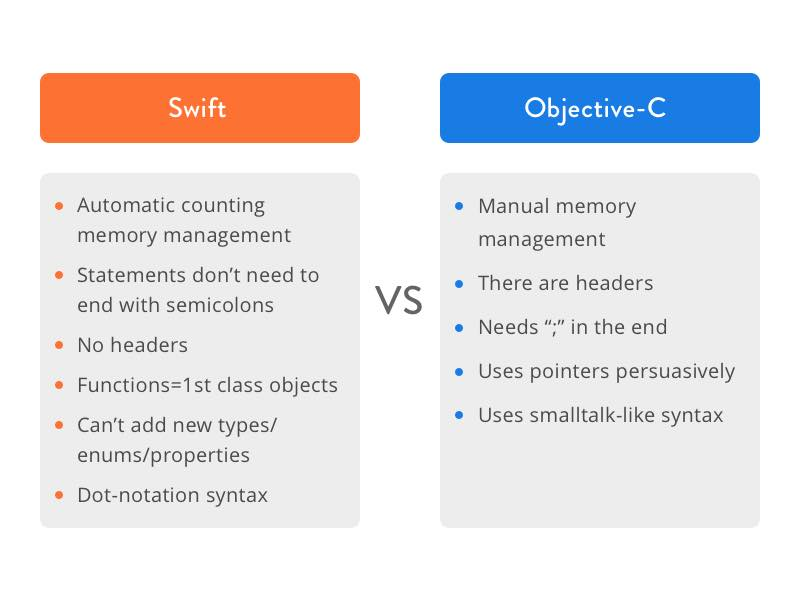
\includegraphics[scale=0.45]{figures/objc_swift.jpg}
\caption{Algunas diferencias entre los dos lenguajes.\label{fig:objc_swift}}
\end{figure}

\subsection{\textit{Alamofire}}
Esta librería \cite{noauthor_alamofire_nodate} fue incluida en el \textit{app iOS} para realizar todas las peticiones \textit{HTTP} necesarias, así como el \textit{streming} de nodos de la base de datos.

\subsection{\textit{Postman}}
Este programa que se puede descargar para \textit{Mac}, \textit{Windows} y \textit{Linux} \cite{noauthor_postman_nodate}. Tiene planes de pago pero para nootros con el gratuito fue suficiente.
Con esta herramienta podemos probar las peticiones antes de incorporarlas a la aplicación, ver que códigos de error se obtienen, etcétera.

\subsection{iOS}
La decisión de hacer una aplicación para \textit{iOS} en lugar de para \textit{Android} se debe a que ya se disponía de las herramientas necesarias (ordenador con sistema operativo \textit{macOS} y un \textit{iPhone}), y sobre todo, al tipo de aplicación que se va a desarrollar.

Los \textit{iPhones} son teléfonos caros y suelen estar en manos de personas con un poder adquisitivo más alto. Como prueba, a pesar de tener un menor número de usuarios que \textit{Android} a nivel mundial, el \textit{App Store} (la tienda de aplicaciones de \textit{Apple}) genera muchos más ingresos que el \textit{Play Store} (tienda de aplicaciones \textit{Android}) \cite{christian_collado_app_2018}. Al ser una aplicación con un propósito consumista, es lógico pensar que tendrá una mayor acogida entre los usuarios de \textit{iOS} que entre los de \textit{Android}.


\section{Tecnologías de edición y gestión}
En esta sección, hablaremos sobre las herramientas de edición utilizadas durante el proyecto:

\subsection{Xcode}
Para crear aplicaciones para \textit{iOS}, es necesario el programa \textit{Xcode}, si se dispone de un ordenador con sistema operativo \textit{macOS}, se puede obtener de manera gratuita. Pero muchas veces no se dispone de este \textit{Hardware}, en este caso hay alternativas \cite{chris_ching_xcode_2017} como instalar dicho sistema operativo en una máquina virtual, o bien alquilar una máquina en la nube.


\subsection{\textit{IconJar}}
Para descargar iconos en formato \textit{PDF}, necesarios para la aplicación, se utilizó el programa \textit{IconJar} \cite{curtis_hard_davey_heuser_iconjar_nodate} en su versión gratuita.
\begin{figure}[tbp]
\begin{center}
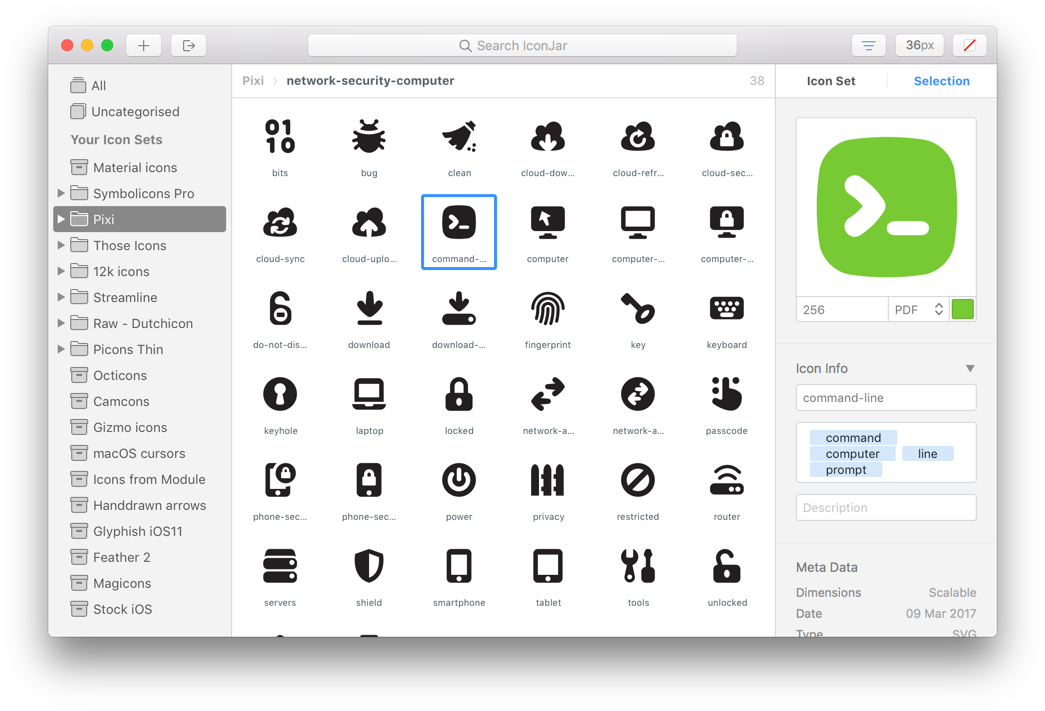
\includegraphics[scale=0.37]{figures/iconjar.png}
\caption{Generación de iconos con \textit{IconJar}.}
\end{center}
\end{figure}

\subsection{\textit{Adobe Xd}}
Para el diseño de pantallas e interfaces, se utilizó el programa \textit{Adobe Xd }\cite{noauthor_adobe_nodate}, también en su versión gratuita.
Para aprender a manejar esta herramienta es recomendable seguir tutoriales \cite{forrestknight_how_nodate}, sobre todo al principio.
Se deben utilizar este tipo de programas para realizar los diseños, porque si intentamos llevarlos a cabo sin planificar, lo que va a pasar es que tengamos que compilar el programa cada vez que realicemos un pequeño cambio. En cambio, si ya sabemos como queremos la \textit{app}, podemos programarlo todo y compilar al final sabiendo que va a quedar bien.

\subsection{\textit{Git}}
Para el control de versiones, se utilizó el \textit{Git} \cite{noauthor_git_nodate} de la facultad. En el cual todos los alumnos podemos entrar con nuestra cuenta y crear proyectos privados de manera gratuita.

\begin{figure}[tbp]
\centering
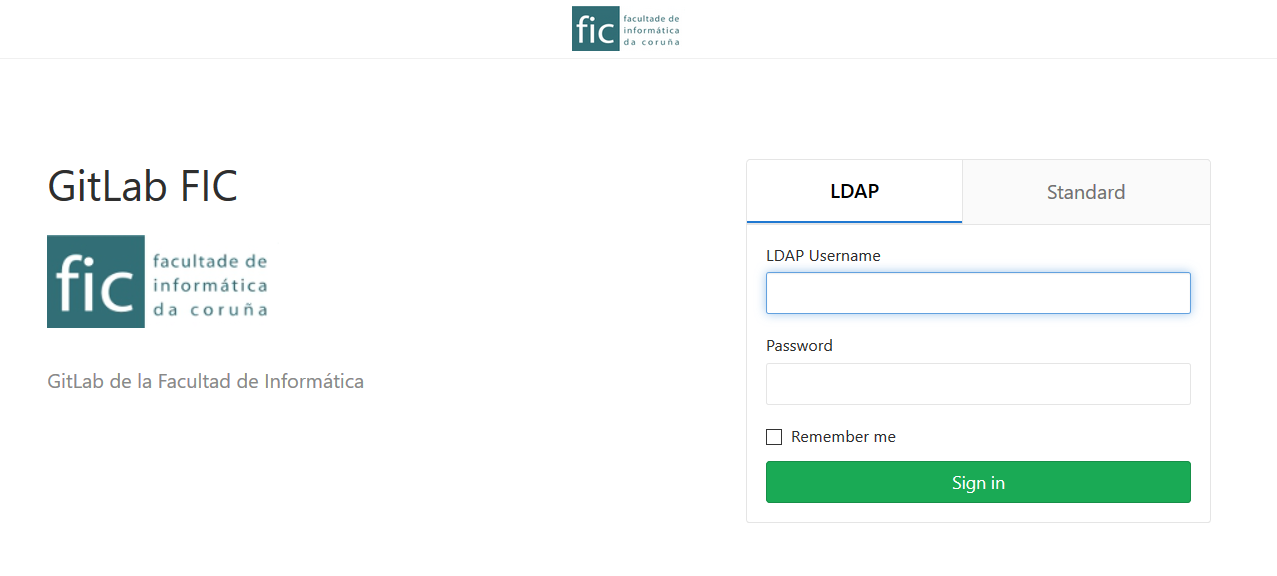
\includegraphics[scale=0.5]{figures/gitfic.png}
\caption{Se inicia sesión con la cuenta de la Universidad}
\end{figure}

\subsection{\textit{LaTeX}}
Para redactar la memoria, se escogió \textit{LaTeX} porque da unos resultados muy elegantes y la complicación es mínima.

Para facilitar la tarea se utilizó una herramienta web llamada \textit{Overleaf} \cite{noauthor_overleaf_nodate} en su versión gratuita. La cual permite compartir el documento con un \textit{link} para que varias personas puedan leerlo y/o editarlo. También lo sube a \textit{Git}, dándonos un enlace mediante el cual podemos clonarlo para guardar una copia en nuestro ordenador personal. Cabe destacar que esta herramienta ofrece la posibilidad de compilar a medida que escribimos, así podemos ver resultados casi inmediatamente.

\subsection{\textit{GanttProject}}
A la hora de elaborar un diagrama de \textit{Gantt} para planificar el desarrollo del proyecto, se optó por utilizar una herramienta de software libre llamada \textit{GanttProject} \cite{noauthor_ganttproject_nodate}. Es una herramienta que ofrece menos funcionalidades que otras como \textit{Microsoft Project}, pero mucho más fácil de usar.

Algunas de las funcionalidades que ofrece son: gráficos \textit{PERT}, creación de informes en formato \textit{PDF} y \textit{HTML}, importación y exportación de documentos en formato \textit{MS Project}, importación y exportación de datos contenidos en hojas de cálculo, creación de diagramas de \textit{Gantt}, jerarquías y dependencias entre tareas, etcétera.
No es la única herramienta de software libre para gestionar proyectos \cite{ruben_alcaraz_3_2012}, aquí podemos encontrar un breve tutorial para iniciarnos con esta herramienta \cite{dmitry_barashev_ganttproject_2011}.
\chapter{Análisis de requisitos}
En este capítulo se hablará sobre los requisitos funcionales y no funcionales, así como de los actores y casos de uso que fueron implementados.
\section{Requisitos funcionales}
Estos requisitos son pedidos por el director de proyecto. Se fueron añadiendo nuevos a medida que avanzaba el desarrollo. La lista inicial de requisitos funcionales sería:
\begin{enumerate}
\item \textbf{Obtención de la posición del usuario:} Para saber en todo momento que ofertas de su interés hay a su alrededor.
\item \textbf{Sistema de roles:} La aplicación tendrá acciones que sólo podrán llevar a cabo determinados usuarios.
\item \textbf{Caja negra nos da nuestra posición:} Al incluir el \textit{SDK} de \textit{Situm} en nuestra aplicación y configurarlo adecuadamente, se envían los datos recogidos por los sensores a \textit{Situm} y nos llega nuestra posición. La forma en que se calcula nos es indiferente.
\item \textbf{Gestión de tiendas y ofertas:} La propia aplicación tiene que permitir dar de alta/baja tiendas y crear/eliminar ofertas.
\item \textbf{Aviso mediante notificaciones:} Para que un usuario sepa que hay una oferta de su interés cerca debe recibir una notificación en su teléfono.
\item \textbf{Canjeo de las ofertas mediante códigos \textit{QR}:} Para dejar constancia de que un usuario a disfrutado de una oferta, con la propia aplicación usuarios con rol de empleado podrán leer los códigos \textit{QR} de los usuarios cliente.
\end{enumerate}
Otros requisitos funcionales que iban apareciendo y que se incorporaron al ciclo de desarrollo \textit{SCRUM} serían:
\begin{enumerate}
\item \textbf{Caducidad de las ofertas:} Nace esta funcionalidad con la intención de motivar al consumidor. Al darle un tiempo limitado a la oferta, crea en él la sensación de que debe aprovechar la oportunidad.
\item \textbf{Número limitado de unidades:} Esta funcionalidad surge con la misma intención que la anterior, se motiva al cliente haciéndole ver en tiempo real como el número de unidades disponibles de una oferta va disminuyendo a medida que la gente va canjeado sus códigos \textit{QR}.
\item \textbf{Atajo de \textit{Siri} para escanear oferta:} durante el desarrollo del proyecto, \textit{Apple} lanza la beta de \textit{iOS} 12, la cual permite asociar acciones de una aplicación con comandos de voz personalizados para ejecutarlos desde \textit{Siri}.\\Se añade al ciclo de desarrollo un nuevo requisito funcional: lanzar el escáner de códigos \textit{QR} utilizando un comando de voz de \textit{Siri}.
\end{enumerate}
\section{Requisitos no funcionales}
Hay otro tipo de requisitos, que no hacen referencia a las funciones de la aplicación. Sino a la manera en que se desempeñan dichas funciones. Estos son llamados requisitos no funcionales, para este proyecto hemos fijado los siguientes:
\begin{enumerate}
\item \textbf{Tiempo real:} La aplicación tiene que comunicarse con \textit{Firebase} en tiempo real, teniendo los datos siempre actualizados sin necesidad de refrescar. De tal manera que las ofertas vayan apareciendo a medida que se crean.
\item \textbf{Sistema distribuido:} La aplicación móvil es la que realiza todo el trabajo. La base de datos simplemente almacena la información y el servicio de \textit{Situm} recoge los datos de nuestros sensores y nos devuelve nuestra posición, como una caja negra. De esta manera, si más adelante queremos utilizar otros servicios, podríamos hacerlo sin realizar grandes cambios en la aplicación.
\item \textbf{Interfaz intuitiva:} La interfaz debe ser sencilla e intuitiva para que el usuario no se sienta abrumado. Además, hay que tener en cuenta que prácticamente todas las aplicaciones \textit{iOS} tienen una línea de diseño que es aconsejable seguir \cite{noauthor_ios_nodate} .
\item \textbf{Recursos del sistema:} Hay que tener en cuenta que la aplicación necesita tener el \textit{Bluetooth}, el \textit{WiFi} y el \textit{GPS} encendidos. La batería puede llegar a verse comprometida durante la ejecución, así que tendremos que programar de manera lo más eficiente posible para compensar.
\end{enumerate}
\section{Actores}
Los usuarios interactuarán de manera diferente con la aplicación, dependiendo del rol que jueguen en la plataforma. Según el rol podrán realizar unas acciones u otras, pero la asignación de permisos es flexible, es decir, al darle permisos a un usuario con rol inferior, podemos darle permisos para todas las acciones o sólo para algunas.
\begin{itemize}
\item \textbf{Cliente sin autenticar:} Usuario que puede utilizar la aplicación para ver las ofertas disponibles, recibir notificaciones de las que tiene a su alrededor. No podrá realizar acciones que requieran autenticación: disfrutar ofertas, indicar si le gustan o no, revisar las ofertas recibidas y canjeadas.
\item \textbf{Cliente autenticado:} Usuario que sí se ha dado de alta y puede realizar las acciones previamente comentadas. Podrá indicar si una oferta le gusta, o si por el contrario, prefiere ignorarla. Las ofertas sólo pueden aplicarse una vez por persona, por ello será necesaria la autenticación para poder disfrutar de ella. No podrá dar permisos a otros usuarios.
\item \textbf{Empleado de tienda:} Usuario autenticado que se encargará de canjear el código \textit{QR} de las ofertas. Cada vez que escanee el código de una oferta, se realizará la acción necesaria en la base de datos, marcándola como disfrutada para ese usuario. No podrá dar permisos a otros usuarios.\\
Quedará registrado en el sistema qué empleado ha canjeado el código \textit{QR}, a qué cliente y la fecha, por motivos de seguridad.
\item \textbf{Propietario de tienda:} Usuario autenticado que podrá crear, eliminar o modificar ofertas dentro de su tienda. También podrá darle permisos de empleado a otro usuario autenticado.
\item \textbf{Gerente de centro comercial:} Usuario autenticado que tiene la capacidad de crear, eliminar o modificar tiendas dentro del centro comercial que administra. También podrá darle permisos de propietario de tienda a otro usuario.
\item \textbf{Administrador de la plataforma:} Usuario autenticado en la aplicación, cuya función característica será la de dar el rol de "Gestor de centro comercial" a aquellos usuarios que lo soliciten. Este individuo también tendrá acceso a la plataforma de \textit{Situm} y a la consola de \textit{Firebase}. Podrá añadir edificios, subir planos, modificar la base de datos a mano y realizar cualquier acción que le permita la plataforma de \textit{Firebase}. 
\end{itemize}
\newcounter{UseCase}
\section{Casos de uso}
A continuación se explican los diferentes casos de uso, separados según que actor los puede llevar a cabo.
\subsection*{Casos de uso del Cliente sin autenticar (CL)}
Este es el usuario que menos acciones podrá realizar, a continuación se presentan los casos de uso más básicos de la aplicación móvil.
\stepcounter{UseCase}
\subsubsection*{CU-\theUseCase-CL Seleccionar un centro comercial:}
Podrá ver un listado de todos los centros comerciales cuyo mapa está subido a la plataforma. Seleccionando uno podrá ver un listado de las tiendas que hay en él.
\stepcounter{UseCase}
\subsubsection*{CU-\theUseCase-CL Seleccionar una tienda:}
Del mismo modo podrá seleccionar una tienda para ver así las ofertas que hay disponibles en esta.
\stepcounter{UseCase}
\subsubsection*{CU-\theUseCase-CL Seleccionar una oferta:}
Una vez en el listado de ofertas, podrá seleccionar una para verla más en detalle, también se le mostrará aquí el código \textit{QR} necesario para canjearla. Si no estuviese autenticado, se le mostraría un botón para iniciar sesión con \textit{Google} en lugar del código \textit{QR}.
\stepcounter{UseCase}
\subsubsection*{CU-\theUseCase-CL Ver mapa de todo el edificio:}
El usuario podrá ver todo el edificio y un icono representando su posición si se encuentra ahí en ese momento. También podrá explorar las diferentes plantas del edificio y ver las ofertas que hay en ellas.
\stepcounter{UseCase}
\subsubsection*{CU-\theUseCase-CL Seleccionar una oferta desde el mapa:}
Las ofertas están representadas por chinchetas en el mapa, así que el usuario podrá seleccionar una para verla más en detalle del mismo modo que la seleccionaba desde la lista.
\stepcounter{UseCase}
\subsubsection*{CU-\theUseCase-CL Ver oferta en el mapa:}
Se abrirá el mapa otra vez, pero sólo mostrando la planta en la que se encuentra la oferta, y solamente su chincheta.
\stepcounter{UseCase}
\subsubsection*{CU-\theUseCase-CL Recibir notificación:}
A medida que cambia su posición, el usuario podrá recibir notificaciones si encuentra ofertas cercanas.
\stepcounter{UseCase}
\subsubsection*{CU-\theUseCase-CL Desactivar las notificaciones:}
Desde la pantalla de perfil, podrá desactivar las notificaciones si no quiere ser molestado.
\stepcounter{UseCase}
\subsubsection*{CU-\theUseCase-CL Silenciar las notificaciones:}
Desde la pantalla de perfil, podrá silenciar las notificaciones si quiere que le sigan llegando pero sin emitir ningún sonido.
\stepcounter{UseCase}
\subsubsection*{CU-\theUseCase-CL Ver oferta en detalle desde la notificación:}
Si se selecciona la notificación se accederá a la aplicación, visualizando en detalle la oferta como si la hubiésemos seleccionado en el mapa o en la lista.
\stepcounter{UseCase}
\subsubsection*{CU-\theUseCase-CL Autenticarse:}
Consiste en la autenticación del usuario mediante una cuenta de \textit{Google}, si ya tiene una en el teléfono no será necesario que introduzca la contraseña. Podrá hacerse desde el detalle de la oferta o en la pantalla de inicio de la aplicación.
\subsection*{Casos de uso del Cliente autenticado (CA)}
Podrá realizar las acciones del usuario sin autenticar y, a mayores, otras que requieren autenticación.
\stepcounter{UseCase}
\subsubsection*{CU-\theUseCase-CA Cerrar sesión:}
Desde la pantalla de perfil, el usuario autenticado podrá cerrar sesión.
\stepcounter{UseCase}
\subsubsection*{CU-\theUseCase-CA Canjear oferta:} Las ofertas tienen asociado un código \textit{QR} para poder canjearlas. Así se controla que un mismo usuario no disfrute varias veces de una oferta que sólo puede canjearse una vez por persona.
\stepcounter{UseCase}
\subsubsection*{CU-\theUseCase-CA Marcar como favorita una oferta:} Desde la pantalla de detalle de oferta, desde el listado de ofertas recibidas y desde el listado de ofertas rechazadas, el usuario podrá indicar que le gusta. Si anteriormente la había rechazado, al indicar que es de su agrado volverá a recibir notificaciones sobre esta.
\stepcounter{UseCase}
\subsubsection*{CU-\theUseCase-CA Rechazar una oferta:} Desde la pantalla de detalle de oferta, desde el listado de ofertas favoritas y desde el listado de ofertas recibidas, el usuario podrá indicar que no le interesa y no se le volverá a notificar.
\stepcounter{UseCase}
\subsubsection*{CU-\theUseCase-CA Ver ofertas favoritas:} El usuario podrá ver un listado de aquellas ofertas que previamente marcó como interesantes, pudiendo seleccionarlas para verlas en detalle y canjearlas. También desde aquí puede indicar que ya no le gustan o eliminarlas de la lista.
\stepcounter{UseCase}
\subsubsection*{CU-\theUseCase-CA Ver ofertas rechazadas:} El usuario podrá ver un listado de aquellas ofertas que previamente rechazó, pudiendo seleccionarlas para verlas en detalle y canjearlas. También desde aquí podrá indicar que sí que le gustan o eliminarlas de la lista.
\stepcounter{UseCase}
\subsubsection*{CU-\theUseCase-CA Ver ofertas canjeadas:} El usuario podrá ver un listado también de todas aquellas ofertas que canjeó. Además en la lista aparecerán indicadas aquellas ofertas que ya fueron canjeadas, para así no volver a intentar canjearlas. Esto además sirve de registro para posible reclamaciones futuras, por lo tanto no podrá eliminar ninguna oferta de la lista, quedarán ahí para siempre.
\stepcounter{UseCase}
\subsubsection*{CU-\theUseCase-CA Ver ofertas recibidas:} El usuario podrá ver un listado de todas las ofertas por las que pasó, a modo de recordatorio, por si acaso no estaba atento al móvil o no tenía activadas las notificaciones. Podrá mandar las ofertas a favoritas o rechazarlas desde esta lista, también podrá eliminarlas de la lista sin ninguna opinión al respecto.
\stepcounter{UseCase}
\subsubsection*{CU-\theUseCase-CA Eliminar oferta de usuario:} Estas ofertas serían todas aquellas que tienen relación con usuario autenticado: favoritas, rechazadas, canjeadas o recibidas. El usuario autenticado podría eliminar una oferta de cualquiera de estas listas (excepto de la de canjeadas), para limpiar la lista o porque le es indiferente. Se le seguiría notificando en caso de volver a cruzarse con ella.
\stepcounter{UseCase}
\subsubsection*{CU-\theUseCase-CA Ver detalle de oferta de usuario:} Si se selecciona una oferta de una de las listas comentadas en los cinco casos de uso anteriores, se muestra el detalle de la misma como si la hubiésemos seleccionado del listado de ofertas de una tienda o a través de una notificación.
\subsection*{Casos de uso del  Empleado de la tienda (ET)}
Además de poder realizar todas las acciones anteriores, también podrá llevar a cabo las siguientes.
\stepcounter{UseCase}
\subsubsection*{CU-\theUseCase-ET Canjear una oferta para un usuario:} A través de la pantalla de perfil, podrá abrir el escáner de códigos \textit{QR} para canjear una oferta a un cliente. Si el escaneo tiene éxito, el usuario no podrá volver a canjearla. El empleado sólo podrá canjear ofertas de la tienda en la que trabaja, cabiendo la posibilidad de que trabaje en varias tiendas.
\stepcounter{UseCase}
\subsubsection*{CU-\theUseCase-ET Canjear una oferta para un usuario a través de \textit{Siri}:} Este caso de uso es idéntico al anterior, salvo por el hecho de que en lugar de abrir el escáner pulsando un botón en pantalla, se abrirá cuando el empleado pronuncie la frase que el mismo asoció a esa acción.
\subsection*{Casos de uso del Propietario de la tienda (PT)}
Las acciones propias de los propietarios de tiendas serían las siguientes:
\stepcounter{UseCase}
\subsubsection*{CU-\theUseCase-PT Crear oferta:}
Podrá crear una oferta con los atributos correspondientes y situándola en el mapa. Sólo podrá crear ofertas en tiendas de su propiedad, cabiendo la posibilidad de que sea propietario de varias tiendas.
\stepcounter{UseCase}
\subsubsection*{CU-\theUseCase-PT Editar oferta:}
El propietario de una tienda podrá modificar cuando crea conveniente cualquiera de los atributos de una oferta de ese establecimiento. Incluso podrá darle más tiempo a una oferta caducada o asignarle nuevas unidades a una oferta ya agotada.
\stepcounter{UseCase}
\subsubsection*{CU-\theUseCase-PT Eliminar oferta:}
Podrá eliminar una oferta si ya no le interesa mostrarla al público. Podrá realizar esta acción en cualquier tienda de la que sea propietario.
\stepcounter{UseCase}
\subsubsection*{CU-\theUseCase-PT Dar rol de empleado a un usuario:} Podrá darle rol de empleado de alguna de sus tiendas a otro usuario que tiene que estar previamente autenticado.
\stepcounter{UseCase}
\subsubsection*{CU-\theUseCase-PT Quitar rol de empleado a un usuario:} Podrá quitarle el rol de empleado a algún usuario al que se lo había dado anteriormente.
\subsection*{Casos de uso del Gestor de centro comercial (GC)}
Las acciones propias de los gestores de centros comerciales serían las siguientes:
\stepcounter{UseCase}
\subsubsection*{CU-\theUseCase-GC Crear tienda:} Podrá crear una tienda dentro de su centro comercial.
\stepcounter{UseCase}
\subsubsection*{CU-\theUseCase-GC Eliminar tienda:} Podrá eliminar una tienda de su centro comercial.
\stepcounter{UseCase}
\subsubsection*{CU-\theUseCase-GC Editar tienda:} Podrá modificar los atributos de una tienda de su centro comercial.
\stepcounter{UseCase}
\subsubsection*{CU-\theUseCase-GC Dar rol de propietario de tienda a un usuario:} Dicho usuario deberá estar previamente autenticado y sólo tendrá permisos sobre dicha tienda.
\stepcounter{UseCase}
\subsubsection*{CU-\theUseCase-GC Quitar rol de propietario de tienda a un usuario:} Podrá quitarle el rol de propietario de tienda a un usuario al que se lo había dado con anterioridad.
\subsection*{Casos de uso del Administrador de la plataforma (AP)}
Los acciones propias de los administradores de la plataforma serán:
\stepcounter{UseCase}
\subsubsection*{CU-\theUseCase-AP Dar rol de gestor de centro comercial:} Podrán dar rol de gestor de centro comercial a un usuario previamente autenticado, en cualquier centro comercial.
\stepcounter{UseCase}
\subsubsection*{CU-\theUseCase-AP Quitar rol de administrador de centro comercial: } Podrán quitar el rol de administrador de centro comercial a un usuario.



\chapter{Metodología de desarrollo}
En este capítulo se explicará la metodología de desarrollo escogida, así como los hechos que motivaron dicha decisión y como se ha aplicado le metodología a nuestro proyecto concreto.
\section{Metodologías ágiles}
Los principales rasgos de una metodología ágil serían los siguientes:
\begin{itemize}
\item Todos los objetivos, fechas límite, decisiones... han de girar en torno al equipo de desarrollo. Las personas serán el centro del proceso y se configurará el entorno según sus necesidades.
\item Se priorizará crear software que funcione correctamente frente a una documentación demasiado detallada.
\item La comunicación con el cliente ha de ser continua y periódica durante todo el proceso, evitando contratos iniciales y una pérdida total de contacto hasta la fecha de entrega.
\item En el desarrollo de software en muy común que surjan imprevistos, es importante tener la capacidad de adaptarse a ellos rápidamente.
\end{itemize}
La localización en interiores es una disciplina cuyas bases no están demasiado asentadas, así que debemos dejar las puertas abiertas a cambios, como por ejemplo nuevas tecnologías o técnicas de obtención de la localización. Una forma inteligente de realizar un proyecto de este tipo, es tratar como una caja negra la obtención de las coordenadas, siendo indiferente para la aplicación como se obtengan. Da igual que sea mediante \textit{GPS}, con la \textit{API} de \textit{Situm} o con cualquier otro servicio. De esta manera, el día de mañana podríamos adaptar el proyecto de manera cómoda a una nueva tecnología, permitiendo a la aplicación evolucionar y no dejándola atrasada por miedo a realizar gran cantidad de cambios.
\subsection*{\textit{SCRUM}}
\textit{Scrum} es una metodología ágil de desarrollo software, está diseñada para equipos de 3 a 9 desarrolladores que dividen el trabajo en iteraciones, llamadas \textit{sprints}. La duración de estos intervalos suele ser de menos de un mes, y suelen realizarse reuniones cortas diarias para analizar el curso que sigue el proyecto.
Cada una de estas iteraciones tiene que proporcionar un resultado completamente funcional, cada una de ellas será una versión del producto final cada vez más avanzada. El proceso completo sigue las siguientes fases:
\begin{enumerate}
\item \label{fase1scrum} primero de todo será una reunión con el cliente para crear una lista de requisitos ordenados por su prioridad, dependiendo del beneficio y del coste de los mismos. Esta lista se elabora con el cliente.
\item \label{fase2scrum} A partir de la lista de requisitos inicial, se selecciona un subconjunto de los mismos que conformarán la siguiente iteración.
\item Se llevan a cabo reuniones periódicas, estas sin el cliente, para poder reaccionar rápidamente ante cualquier problema o requisito que vaya surgiendo a lo largo del desarrollo.
\item El último día de la iteración se lleva a cabo otra reunión, en la cual, sí que se encuentra el cliente. Aquí se analizará el trabajo realizado y los problemas surgidos durante el desarrollo, para que no se vuelvan a repetir en los siguiente sprints.
\item Finalmente, hay que garantizar que el producto que se entrega al cliente sea un software completamente funcional. Si se desea continuar desarrollando más sprints, se repite el proceso desde la fase \ref{fase2scrum}.
\end{enumerate}
\section{Adaptación a nuestro proyecto}
Se ha elegido esta metodología porque las características del equipo de desarrollo son muy diferentes al de una empresa real. La plantilla de programadores consta de un solo integrante y el rol de cliente se jugó a partes iguales por el tutor y por el alumno. Ya que ambos propusieron nuevas metas y objetivos a medida que avanzaba el proyecto, y además, no sólo se realizaron reuniones con el cliente al comienzo y al final de cada \textit{Sprint}, sino que fueron más numerosas.
\subsection*{Roles}
Aquí explicaremos los principales roles de una metodología \textit{SCRUM} y quien los ha representado en este proyecto.
\subsection*{Desarrollo}
\begin{itemize}
\item \textbf{El cliente:} Es el que añade, elimina o prioriza requisitos. Este rol lo ha desarrollado el director del proyecto pero como se comenta anteriormente, es este caso en particular, muchos requisitos también fueron diseñados por el alumno.
Conformarán el total de requisitos que tendrá el proyecto, lo que se llama \textit{Product Backlog}, más tarde, cuando se creen los \textit{sprints}, se hará un estudio de las prioridades de cada uno de estos requisitos y se crearán subconjuntos del \textit{Product Backlog} llamados \textit{Sprint Backlogs}.
\item \textbf{El \textit{Scrum master}:} Tiene el papel de orientar al equipo de desarrollo y de controlar que se sigan las directrices de dicha metodología. Este papel recayó sobre el director del proyecto.
\item \textbf{El equipo de desarrollo:} El alumno llevó a cabo todas las tareas correspondientes del equipo de desarrollo. El análisis de requisitos, la implementación de los mismos y posteriormente las pruebas y la documentación.
\end{itemize}
\subsection*{Plazos temporales}
Los \textit{Sprints} tuvieron una duración aproximada de un mes cada uno, las reuniones diarias no tenían sentido al ser el equipo de desarrolladores integrado solamente por el alumno. Con el cliente nos reunimos con más frecuencia de lo habitual (cada una o dos semanas), pero era necesario, al no haber una figura de analista en el proyecto. Podría decirse que se volvió a la fase \ref{fase1scrum} de la metodología \textit{SCRUM} varias veces, ya que en múltiples ocasiones aparecieron requisitos nuevos a medida que avanzaba el proyecto y hubo que incluirlos en las iteraciones.\\
Es uno de los conceptos principales de la metodología \textit{SCRUM}, la retrospectiva, volviendo a añadir requisitos nuevos al \textit{Product Backlog} a medida que aparecen, dándoles una prioridad determinada y distribuyéndolos en \textit{Sprint Backlogs}.
\begin{figure}[H]
\begin{center}
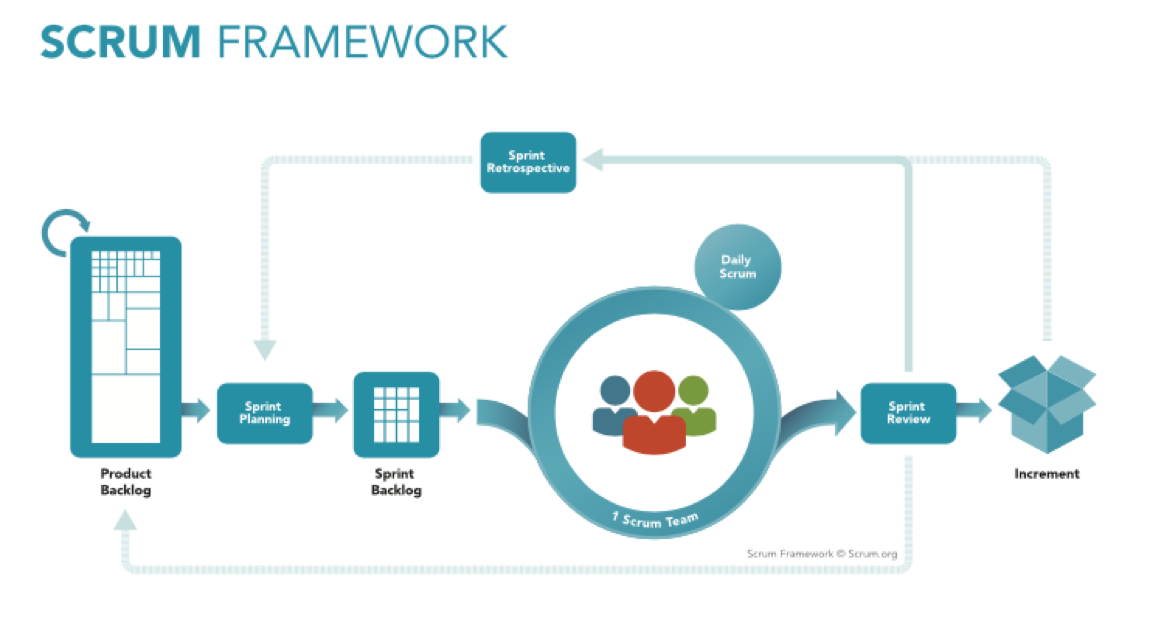
\includegraphics[scale=0.3]{figures/scrum.png}
\caption{Esquema gráfico que explica el funcionamiento de SCRUM.}
\end{center}
\end{figure}

\chapter{Planificación y costes} \label{planificacion_chap}
En este capítulo se comentará los requisitos que se diseñaron inicialmente y la descomposición del proyecto en \textit{Sprints}. Se hablará sobre los costes del proyecto (humanos y materiales) y se analizarán los resultados de cada \textit{Sprint} por separado. 
\section{Recursos}
En esta sección se enumerarán los recursos de los que se dispuso para la realización del proyecto. Habrá tres apartados: humanos, materiales y \textit{Software}.
\subsection*{Recursos humanos}
Los recursos humanos en este proyecto han sido muy pocos, como hemos venido comentando hasta ahora. Constarían de:
\begin{itemize}
\item \textbf{El jefe de proyecto:} En este caso es el profesor, tutor de este trabajo de fin de grado. Realizó las tareas de supervisión, \textit{Scrum Master} y analista.
\item \textbf{El equipo de desarrollo:} en este caso está conformado simplemente por el alumno. El cual tuvo que realizar todas las tareas de análisis, diseño, implementación, pruebas y documentación.
\end{itemize}
\subsection*{Recursos materiales}
En cuanto a los recursos materiales empleados, se dispuso de las siguientes herramientas:
\begin{itemize}
\item Ordenador con sistema operativo \textit{macOS}, imprescindible para programar aplicaciones para dispositivos móviles con sistema operativo \textit{iOS}. El modelo concreto fue un \textit{MacBook Pro} de 2017 con sistema operativo \textit{macOS High Sierra}. Al ser portátil, facilitó el transporte a las reuniones con el director de proyecto, así como permitió trabajar en cualquier lugar.
\item \textit{Smartphone} de la marca \textit{Apple} con sistema operativo \textit{iOS} 12 beta, sirvió para realizar pruebas de la aplicación sobre un dispositivo real. El modelo concreto es un \textit{iPhone SE}.
\item \textit{Beacons} utilizados para calibrar el entorno, aunque podrían haberse prescindido de ellos ya que se puede calibrar solamente con \textit{WiFi}. El modelo concreto es \textit{iBSK105} de la marca \textit{Accent Systems}.
\end{itemize}
\subsection*{Recursos software}
\begin{itemize}
\item \textit{IDE} para programar aplicaciones \textit{iOS}, el programa se llama \textit{Xcode} y sólo puede ejecutarse en máquinas con \textit{macOS}.
\item Simuladores para ejecutar y probar la aplicación más rápidamente sin necesidad de utilizar un dispositivo físico, el \textit{IDE} comentado anteriormente ya incluye simuladores de gran cantidad de \textit{iPhones} y \textit{iPads} con diversas versiones de \textit{iOS}.
\item Programas para la generación de iconos en formato \textit{PDF}, se ha elegido la aplicación \textit{IconJar} en su versión gratuita de prueba y fue suficiente para descargar una cantidad importante de iconos en varios colores.
\item Programas de diseño de interfaces de aplicaciones móviles, en este proyecto se utilizó \textit{Adobe Xd} en su versión gratuita.
\item El programa \textit{Postman} que fue utilizado para probar todas las peticiones antes de su incorporación definitiva al proyecto, en su versión gratuita.
\item Plataforma \textit{online} ofrecida por \textit{Firebase}, en este caso en particular hemos utilizado las funcionalidades de base de datos, de autenticación y de ejecución de código \textit{Backend}, pero tiene muchas más.
\item Plataforma \textit{Situm} para la gestión de mapas interiores, para calibrar sus entornos y obtener la posición en los mismos. Tiene varias herramientas, pero en este caso se han utilizado el \textit{Dashboard} para subir los planos y la aplicación móvil para \textit{Android} \textit{SitumMapsTool} para calibrar los entornos.
\end{itemize}

\section{Planificación inicial}
En esta sección se muestra la descomposición en \textit{sprints} del proyecto y sobre como se llevó a cabo un desarrollo incremental, obteniendo resultados funcionales al final de cada iteración.
En la figura~\ref{fig:gantt_inicial} se puede ver la representación temporal de los \textit{sprints} y sus correspondientes hitos, a lo largo del tiempo.
\begin{figure}[tbp]
\begin{center}
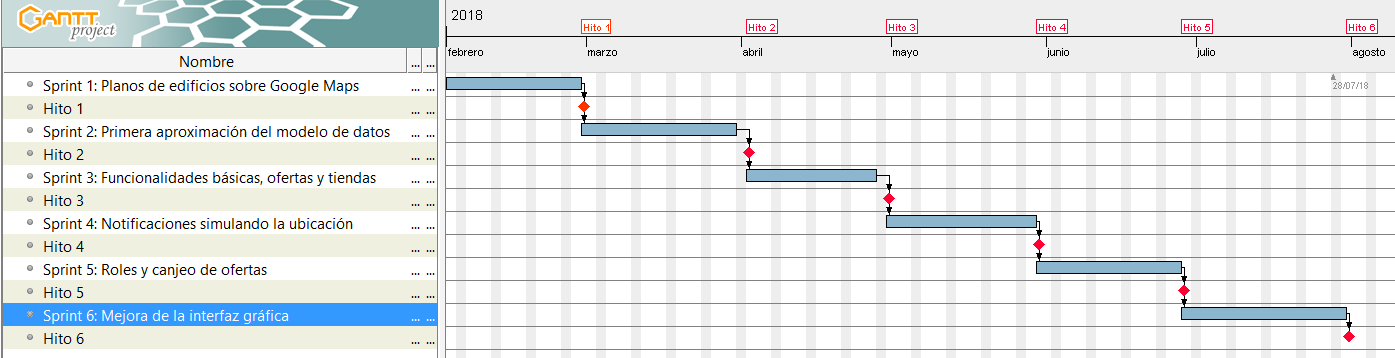
\includegraphics[scale=0.5]{figures/ganrr.png}
\caption{Diagrama de \textit{Gantt} de la planificación inicial.
\label{fig:gantt_inicial}}
\end{center}
\end{figure}

\subsection{\textit{Sprint} 1: Prototipo \textit{iOS} con localización en interiores}
En este \textit{sprint}, se suben a \textit{Situm} los planos interiores de varios edificios y se crea una aplicación móvil sencilla que obtiene estos planos y los superpone sobre un mapa de \textit{Google Maps}. Básicamente se sustituye el sistema de mapas interiores de \textit{Google} por uno propio, creando unos botones que permiten cambiar de piso y una caché que almacena las imágenes descargadas de \textit{Situm}. El \textit{sprint} se descompone en las siguientes tareas:
\begin{itemize}
\item Obtención de las \textit{API Keys} de \textit{Situm} y de \textit{Google Maps} para poder añadir estos servicios a nuestra aplicación.
\item Se sigue la guía para incorporar el \textit{SDK} de la plataforma \textit{Situm} a la aplicación \textit{iOS}. En este manual se indica como descargar todos los edificios y la información relativa a ellos: nombre, plantas, planos, etcétera.
\item Una vez obtenidos los edificios, sus planos se superponen sobre el mapa, sustituyendo los planos de interiores de \textit{Google} por los de \textit{Situm}. Hay que desarrollar toda una lógica para moverse entre los pisos del edificio, cambiar de edificio, cachear las imágenes, etcétera.
\end{itemize}
\textbf{Hito 1:} Como resultado de este \textit{sprint} se obtiene una aplicación muy sencilla pero plenamente funcional que se enseña al director del proyecto. Viendo que permite obtener la información de los edificios, montar sus planos sobre un mapa de \textit{Google Maps}, y que cambia de piso sin problema, se podrá continuar con las siguientes iteraciones.

\subsection{\textit{Sprint} 2: Creación del modelo inicial de datos}
En este \textit{sprint} se empezará a diseñar la estructura con la que se almacenan los datos en \textit{Firebase}: ofertas, tiendas, centros comerciales, permisos y usuarios. Se descompone en las siguientes tareas:
\begin{itemize}
\item Obtención de una \textit{API Key} de \textit{Firebase} y dada de alta de la aplicación 
\item Estudio de las posibilidades que ofrece \textit{Firebase} para almacenar y recuperar los datos. En este caso, se escogió el servicio más sencillo: la \textit{API REST} de \textit{Firebase}.
\item Autenticación del usuario y almacenamiento en \textit{Firebase}. Se lleva a cabo con una cuenta de \textit{Google} y el usuario se da de alta en la plataforma de \textit{Firebase}.
\end{itemize}
\textbf{Hito 2:} reunión con el director para comentar el modelo y ver que problemas podrían surgir a la larga. Aunque en este \textit{sprint} planteamos un diseño inicial del modelo, es muy probable que a medida que se desarrolla la aplicación, aparezcan nuevas necesidades \cite{firomero87_relaciones_nodate}.

\subsection{\textit{Sprint} 3: Funcionalidades básicas: Mapas, ofertas y tiendas}
Aquí se desarrollarán las funcionalidades más básicas de la aplicación, para no tener que tocar manualmente la base de datos de \textit{Firebase}. 
Además se separará del resto de la aplicación la parte en la que se hacen las peticiones, para que cambios posteriores en el modelo no obligasen a realizar cambios también en todo código.
\begin{itemize}
\item Añadir y eliminar ofertas, tiendas y roles.
\item Situar las ofertas en el mapa y permitir la visualización en detalle de las mismas al seleccionarlas.
\item También se visualizarán en formato lista las tiendas y las ofertas, pudiendo acceder al detalle de estas también a través de la lista.
\end{itemize}
\textbf{Hito 3:} Comprobación de que todas las peticiones hacen lo esperado, primero utilizando la herramienta \textit{Postman} y posteriormente a través de la propia aplicación.

\subsection{\textit{Sprint} 4: Simulación de la posición y notificaciones}
Debido a una limitación de los dispositivos con sistema operativo \textit{iOS}, no se puede obtener datos sobre al intensidad de la señal recibida de los distintos puntos de acceso \textit{WiFi} del entorno. Esto fue un grave impedimento, ya que la única alternativa que nos quedaba era poner beacons \textit{BLE} en un edificio y dejarlos ahí, habiendo riesgo de robo de los mismos, por ello se descartó esta opción. No sólo eso, sino que además es incómodo tener que ir a pasear a un centro comercial para probar la aplicación, así que hubo que buscar una solución a estos problemas para poder seguir con el desarrollo \textit{software}:
\begin{itemize}
\item Se creará un fichero en formato \textit{JSON} con una sucesión de coordenadas (cada una acompañada del número de piso correspondiente). La aplicación lee este fichero en lugar de leer nuestra posición real (o la proporcionada por \textit{Situm}) y situará nuestra posición en el mapa. De esta manera podemos simular un paseo por el centro comercial sin necesidad de levantarnos de la silla, y sin necesidad de calibrar cada entorno que queremos probar.
\end{itemize}
Además en este \textit{sprint} también se desarrollará toda la lógica de las notificaciones, lanzándolas cuando nos encontremos en el radio de acción de una oferta:
\begin{itemize}
\item Abrir detalle de la oferta a través de la notificación.
\item Gestión de las notificaciones: vibración, sonoras, silenciosas, etcétera.
\end{itemize}
\textbf{Hito 4:} Reunión con el director de proyecto para evaluar el funcionamiento de la simulación y las notificaciones: se comprobará que se generan las notificaciones apropiadas cuando se simula que el cliente está cerca de una oferta, que el usuario puede rechazar una notificación, que se listan las ofertas rechazadas, etc.

\subsection{\textit{Sprint} 5: Implementación de los roles y canjeo de ofertas}
En esta iteración se trabajará en la asignación de roles, y se limitará el acceso de los usuarios sin permisos a diversas acciones. También se incluirá en este \textit{sprint} la funcionalidad de canjear ofertas mediante códigos \textit{QR}:
\begin{itemize}
\item Limitación de las acciones dependiendo del rol.
\item Canjeo de ofertas mediante la lectura de códigos \textit{QR}.
\end{itemize}
\textbf{Hito 5:} En esta reunión se comprueba que un usuario no puede realizar acciones de otros roles y que se canjean bien las ofertas. La aplicación quedaría lista desde el punto de vista funcional ya que sólo faltaría darle un lavado de imagen.

\subsection{\textit{Sprint} 6: Funcionalidades nuevas que irán surgiendo durante el desarrollo y mejora de la interfaz gráfica}
Una de las propiedades de una metodología ágil como \textit{SCRUM} es que van surgiendo nuevos requisitos a lo largo de todo el ciclo de desarrollo. Con estas requisitos que no formaban parte de los iniciales, se conformará un \textit{Sprint backlog} que se dejará para el final, en caso de que dé tiempo.

Además, también se implementará el diseño final de las interfaces de la aplicación. Hasta ahora nos hemos centrado en lo funcional y hemos relegado la estética a un segundo plano. Pero una buena interfaz gráfica tiene gran importancia así que se terminará en el último \textit{sprint}, con todas las funcionalidades ya implementadas.
\begin{itemize}
\item Pantallas de carga, para las operaciones que no sean instantáneas.
\item Animaciones.
\item Elección de las fuentes, colores, proporciones, etcétera.
\end{itemize}
\textbf{Hito 6:} Reunión final y obtención del visto bueno para presentar el proyecto.

\subsection{Preparación de la memoria y pruebas finales}
El último mes se dedicará a la elaboración de la memoria, para la cual ya se habrán ido tomando notas a lo largo de todo el proyecto. También es en esta etapa cuando se realizarán unas últimas pruebas para comprobar que todo el sistema funciona correctamente.




\section{Riesgos y planes de contingencia}
En esta sección se valoran los posibles problemas que pueden surgir durante la utilización de la plataforma. Para valorar la gravedad de estas incidencias se tendrá en cuenta la exposición al riesgo, cuyo valor viene dado no sólo por la probabilidad de que se materialice el riesgo, sino también por el impacto que tendría el mismo si se llegase a materializar.

\subsection{Estimación de riesgos}
Los riesgos que se han tenido en cuenta han sido los siguientes:
\begin{enumerate}
\item \textbf{La aplicación no funciona sin conexión a \textit{Internet}:} Cortes en la conexión, mala cobertura, bajas velocidades y otros problemas relacionados, pueden provocar que la aplicación no funcione de manera fluida. Pero hoy en día, cada vez es más común que la gente tenga buena conexión en sus teléfonos e incluso cuando la aplicación no carga correctamente, nadie le echa la culpa al desarrollador, sino más bien a la compañía telefónica o a la falta de \textit{datos}.
\item \textbf{La aplicación necesita tener el \textit{Bluetooth} activado para funcionar:} Esto puede provocar que muchas personas no quieran tenerla ejecutándose en sus teléfonos, sobre todo cuando les queda poca batería.
\item \textbf{Dependemos mucho de servicios externos:} Esto puede hacer que escalar la aplicación debido a incrementos en el número de usuarios, pueda llegar a producir cortes de servicio al superar los límites contratados. Además de que cualquier problema en las plataformas \textit{Situm} o \textit{Firebase} dejaría inutilizada nuestra plataforma.
\item \textbf{Las empresas que usen la plataforma tendrán que dejar sus datos en nuestras manos:} Tanto los planos como los datos sobre tiendas, ofertas, usuarios, permisos, etcétera. Se almacenan en las cuentas de \textit{Situm} y \textit{Firebase} a las que sólo el administrador de la plataforma tiene acceso. Esto puede resultar un problema desde el punto de vista de la privacidad para muchas empresas, que podrían prescindir de nuestros servicios por este motivo.
\item \textbf{Demasiadas notificaciones:} las notificaciones juegan un papel muy importante en el funcionamiento de esta aplicación. Esto puede llegar a ser pesado para algunas personas que pueden acabar desinstalando la aplicación por considerarla invasiva.
\item \textbf{Difícil incentivar al usuario para que la instale:} A las empresas les encanta publicitarse para atraer clientes potenciales, lo complicado es convencer a los consumidores para que acepten recibir publicidad.
\item \textbf{El cliente puede intentar hacer trampas:} Haciéndole una captura de pantalla a un código \textit{QR} para canjearlo más de una vez, después de que caduque o una vez agotadas las existencias.
\end{enumerate}

\subsection{Planes de contingencia}
Aquí hablaremos sobre posibles soluciones para los problemas anteriormente comentados:
\begin{enumerate}
\item \textbf{Cachear todo lo que se pueda:} Para evitar el problema de consumo de \textit{datos} y los cortes producidos por la falta de conexión a Internet, se debe cachear todo lo posible: planos de edificios, información sobre ofertas, tiendas, etcétera. \textit{Firebase} permite hacer esto muy bien ya que nos permite obtener un dato y suscribirnos a él, es decir: cuando este dato cambie seremos notificados y no antes. De esta manera no tendremos que estar pidiendo los datos (imágenes, texto, códigos \textit{QR}, ofertas de una tienda, ...) para saber si han cambiado sino que los tendremos siempre actualizados.
\item \textbf{Recordarle al usuario que se utilizará \textit{BLE}:} Cuando le pidamos permiso al usuario para la utilización de \textit{Bluetooth}, explicarle que la aplicación utilizará \textit{Bluetooth Low Energy}, el cual tiene un consumo de energía mucho más reducido que el \textit{Bluetooth Classic} y que no agotará la batería tan rápido como piensa.
\item \textbf{Estar atento al crecimiento del número de usuarios:} El administrador de la plataforma debería observar como crece este dato para poder contratar planes \textit{premium} si fuesen necesarios, de esta forma nunca se produciría un corte por culpa de la tarifa. También es recomendable tener trato con ellos para que nos mantengan al tanto si va a estar caído el servicio durante un periodo de tiempo, o cualquier otro inconveniente.
\item \textbf{Rediseño de \textit{Backend}:} Este problema es muy complicado de resolver con el plantemiento actual, en el cual tenemos una sola cuenta de \textit{Situm} y otra de \textit{Firebase}, a las cuales sólo tiene acceso el administrador de nuestra plataforma. Un posible planteamiento sería darle a cada centro comercial sus propias cuentas de \textit{Situm} y de \textit{Firebase}, pero habría que hacer un nuevo análisis de requisitos e incluso sentarse a hablar con \textit{Situm} para que hiciesen algunos cambios en el \textit{SDK}.
\item \textbf{Permitir al usuario bloquear las notificaciones: } Actualmente el sistema operativo iOS permite bloquear o silenciar notificaciones, no sólo eso, sino que la propia aplicación sólo emite sonido la primera vez que pasa al lado de una oferta, las siguientes veces que se cruza con ella no emite ningún sonido para evitar un bombardeo al usuario.
En el sistema operativo \textit{iOS} 12 lanzaron una importante mejora en este aspecto: la aplicación no pregunta si quieres recibir notificaciones hasta que se lanza la primera notificación, de esta manera permite al usuario obtener una de prueba para así decidir si quiere que se le envíen más o no. Esto es muy útil porque hasta ahora las aplicaciones que enviaban notificaciones, tenían que pedir este permiso nada más iniciarse la aplicación, esto disuadía a mucha gente.
\item \textbf{Técnicas de \textit{marketing}:} Hacer que la aplicación sea atractiva para los usuarios es la parte más importante. La aplicación deja la puerta abierta a los propietarios de los establecimientos en este aspecto: ellos pueden decidir el radio de acción de sus ofertas, las horas que van a estar activas y la cantidad de usuarios que van a poder canjearla.
\end{enumerate}


\section{Seguimiento de la planificación inicial}
En esta sección, pondremos de manifiesto como se han desarrollado las iteraciones. Si han surgido problemas, si ha ido todo según lo planeado o, si por el contrario, ha habido algún problema que ha llevado más tiempo de lo normal y que ha habido que mover para el siguiente \textit{sprint}:
\begin{itemize}
\item \textbf{\textit{Sprint} 1:} En esta iteración todo sale según lo previsto ya que encontramos gran cantidad de información y tutoriales por parte de \textit{Situm} y de \textit{Google}. Cabe destacar que quizás se perdió mucho tiempo recortando, editando y subiendo planos a la plataforma de \textit{Situm}. Aunque un desarrollador \textit{software} no es la persona más indicada para esta tarea, sino que más bien un diseñador gráfico o alguien que entienda de mapas, el equipo de desarrollo de este proyecto está integrado por una única persona y no quedó más remedio. 

Cabe destacar, que al final se contactó con \textit{Situm} para que nos importara en nuestra cuenta unos edificios de los que ya tenían los mapas correctamente subidos.
\item \textbf{\textit{Sprint} 2:} En este \textit{sprint} hubo que darle bastantes vueltas a la estructura de la base de datos. Al principio, se empezó utilizando una estructura ineficiente, a medida que avanzaba la aplicación se iban acumulando problemas como el replicamiento de datos o la mala gestión de los identificadores. Así que hubo que rehacerlo todo para que fuese eficiente y escalable, la planificación en esta iteración consumió mucho tiempo.
\item \textbf{\textit{Sprint} 3:} Una vez la estructura de datos era estable se pudo empezar con las funcionalidades básicas. Esta iteración no presentó mayor problema. Cabe destacar que al principio las peticiones a la base de datos no estaban separadas del resto del código, pero hubo que parar y aislarlas, de tal manera que funcionasen como una caja negra para el resto de la aplicación. Quedando así un código mucho más legible y escalable.
\item \textbf{\textit{Sprint} 4:} Aquí sufrimos un pequeño retraso, ya que el \textit{SDK} de \textit{Situm} para \textit{iOS} no permite simular ubicaciones (en \textit{Android} si que existe esta funcionalidad). Entonces para seguir probando y desarrollando la aplicación, decidimos ponernos en contacto con \textit{Situm}, los cuales se pusieron a trabajar en ello. Pero para no retrasar el \textit{sprint} y quedarnos parados, decidimos crear nuestro propio sistema de simulación mediante un fichero \textit{JSON} con posiciones que se lee desde el código. En esta iteración también se llevó a cabo el desarrollo de las notificaciones, durante el cual no hubo ningún problema destacable.
\item \textbf{\textit{Sprint} 5:} En este \textit{sprint}, se desarrolló una primera aproximación en la cual no había roles definidos, simplemente había acciones y a un usuario se le asignaban las acciones que podía llevar a cabo y las que no. Pero tras una reunión con el director de proyecto, hubo que cambiar de estrategia, marcando unos roles bien definidos. De esta manera hay una jerarquía y un usuario no puede dar permisos de un rol superior o igual al suyo, solo inferior. Esto ya se hacía antes, pero de una forma mucho más compleja y menos clara.

Viendo que no íbamos demasiado mal de tiempo, decidimos realizar algunas tareas que se habían ido quedando en el tintero. Como por ejemplo, el canjeo de las ofertas mediante códigos \textit{QR} desde la propia aplicación, incorporando aquí una funcionalidad beta de \textit{iOS} 12: los atajos de \textit{Siri}.
\item \textbf{\textit{Sprint} 6:} 
Se aprovechó el último \textit{sprint} para realizar algunas tareas que se habían ido quedando en el tintero, como las siguientes:
\begin{itemize}
\item Canjeo de las ofertas mediante códigos \textit{QR} desde la propia aplicación, el escáner es activable mediante atajos de \textit{Siri}.
\item Las ofertas caducan, indicar al crear una oferta el tiempo que va a durar.
\item Las ofertas se agotan, indicar al crear una oferta las unidades que se van a lanzar de la misma.
\item Mejorar el perfil de usuario, las listas de ofertas recibidas, rechazadas, canjeadas y recibidas. Permitir configurar las notificaciones: silenciarlas o desactivarlas.
\end{itemize}

Finalmente, hubo que darle un lavado de cara a la aplicación ya que hasta ahora nos habíamos fijado más en el aspecto técnico y no tenía una apariencia atractiva para el usuario. Muchas veces se puede pensar que esto es lo más fácil, pero puede llegar a complicarse bastante. Sobre todo, por el hecho de que hay que probar cada pequeño cambio que se hace y muchas veces, un cambio pequeño que se hace en el código no tiene el efecto deseado sobre la aplicación.
\end{itemize}

En la figura~\ref{fig:gantt_final} se observa la duración  temporal final de los diferentes \textit{sprints}.
\begin{figure}[tbp]
\begin{center}
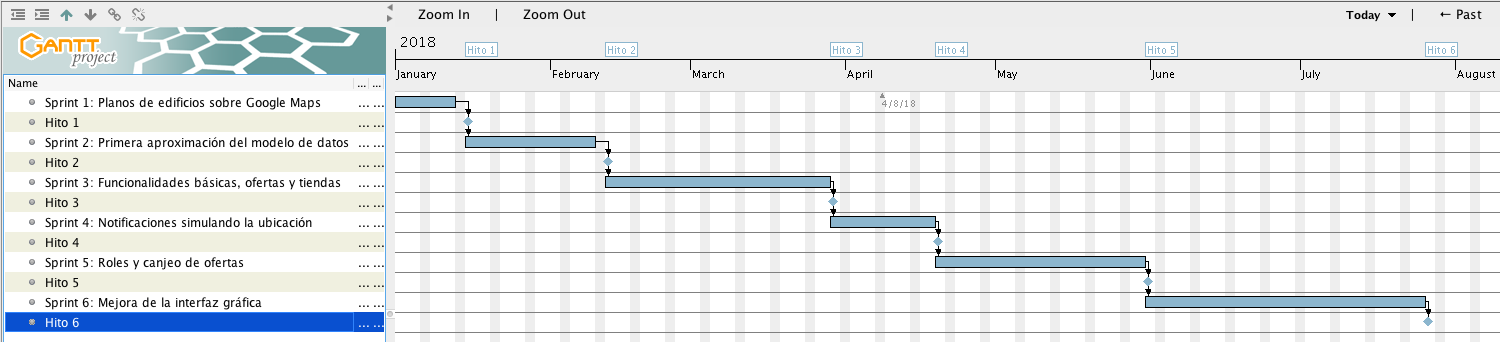
\includegraphics[width=\textwidth]{figures/gantt-final.png}
\caption{Diagrama de \textit{Gantt} final del proyecto.
\label{fig:gantt_final}}
\end{center}
\end{figure}

\section{Evaluación de costes}
A partir de la planificación inicial y de los recursos materiales y humanos necesarios, podemos hacer una estimación de lo que valdría el proyecto en un entorno empresarial.

\subsection{Costes materiales y \textit{software}}
En este proyecto hemos utilizado materiales de los que ya disponíamos y que además ya se encontraban amortizados en el momento de su utilización.
El \textit{software} utilizado también fue gratuito, o bien de pago en su versión de prueba.
Pero hay que mencionar a parte los servicios de \textit{Firebase Database}, \textit{Google Maps} y \textit{Situm}. Ya que en caso de que la aplicación quisiese lanzarse al público, habría que contratar unas tarifas que dieran soporte a mayor número de usuarios, a continuación unas tablas que muestra sus precios:
\begin{table}[btp]
\begin{center}
\small
\begin{tabular}{|l|l|l|l|}
\hline 
& Plan Spark & Plan Flame & Plan Blaze \\
\hline \hline
Precio & Sin cargo & USD 25/mes & Pago por uso \\ \hline
Conexiones simultáneas & 100 & 100.000 & 100.000 por  base de datos \\ \hline
GB almacenados & 1 GB & 2,5 GB & USD 5/GB   \\ \hline
GB descargados & 10 GB/mes & 20 GB/mes & USD 1/GB   \\ \hline
Varias bases de datos  & No & No & Sí  \\ \hline
\end{tabular}
\caption{Precios de \textit{Firebase Database}.}
\label{precios:firebase_db}
\end{center}
\end{table}

\begin{table}[btp]
\begin{center}
\small
\begin{tabular}{|l|l|c|}
\hline 
& Uso mensual gratis & Precio  \\
& (por valor de USD 200) &  por cada mil llamadas \\
\hline \hline
Mapas estáticos & 100.000 cargas & USD ~2 \\ \hline
Mapas dinámicos & ~28.000 cargas & USD ~7 \\ \hline
Street View Estático & ~28.000 panorámicas & USD ~7   \\ \hline
Street View Dinámico & ~14.000 panorámicas & USD 14   \\ \hline
\end{tabular}
\caption{Precios de \textit{Google Maps} de 0 a 100.000 llamadas mensuales.}
\label{precios:googlemaps}
\end{center}
\end{table}

Cuando el intervalo de llamadas mensuales está entre 100.000 y 500.000 a la \textit{API} de \textit{Google Maps}, los precios por cada mil llamadas disminuyen un 20 por ciento con respecto al intervalo 0 - 100.000. Y cuando las llamadas mensuales superan los 500.000, entonces debemos ponernos en contacto con ventas para estipular el precio.

\begin{table}[t]
\begin{center}
\small
\begin{tabular}{|l|c|c|}
\hline 
& Estándar & Premium \\
\hline \hline
Precio & Gratis & 29,90 euros/mes \\ \hline
Posicionamiento preciso 3D & Sí & Sí \\ \hline
Navegación interior paso a paso & Sí & Sí \\ \hline
Creación/subida de ilimitados edificios/mapas & Sí & Sí   \\ \hline
Creación de Puntos de Interés, interiores y exteriores & Sí & Sí  \\ \hline
Creación de Rutas convencionales y accesibles & Sí & Sí   \\ \hline
Generación de eventos/Diseño estrategia geomarketing & Sí & Sí   \\ \hline
Análisis de informes y estadísticas de uso & Sí & Sí  \\ \hline
Visualización de usuarios en tiempo real & Sí & Sí  \\ \hline
Disponible sólo para evaluación & Sí & Sí   \\ \hline
Uso comercial & No & Sí   \\ \hline
Soporte premium & No & Sí   \\ \hline
Alta disponibilidad & No & Sí   \\ \hline
Servicio para empresas & No & Sí   \\ \hline
\end{tabular}
\caption{Precios de \textit{Situm}.}
\label{precios:situm}
\end{center}
\end{table}

\paragraph{Tarifas \textit{Postman}}
Se ha utilizado la versión gratuita de este programa y fue más que suficiente. Pero también tiene opciones de pago  (figura~\ref{fig:postman_pricing}).

\paragraph{Tarifas \textit{Adobe Xd}}
La herramienta de diseño \textit{Adobe Xd} puede utilizarse de manera gratuita, pero también hay opciones de pago que ofrecen funcionalidades más amplias (tabla~\ref{fig:adobe_pricing}).

\begin{table}[t]
\begin{center}
\small
\begin{tabular}{|l|c|c|c|c|}
\hline 
Plan & Precio & Llamadas incluidas & Llamadas & Llamadas\\
& (usuario/mes) & por mes & a mayores & bajo demanda\\ \hline \hline
Postman & 0 USD & 1000 al mes & - & - \\ \hline
Postman & 8 & 10000 & 20 USD/mes & 0.75 USD\\
Pro & USD & al mes & por 50000 &  por 1000\\ \hline
Postman & 18 & 100000 & 20 USD/mes & 0.75 USD\\ 
Enterprise & USD & al mes & por 50000 & por 1000 \\ \hline
\end{tabular}
\caption{Tarifas y planes de uso de la herramienta \textit{Postman}.}
\label{fig:postman_pricing}
\end{center}
\end{table}

\begin{figure}[t]
\centering
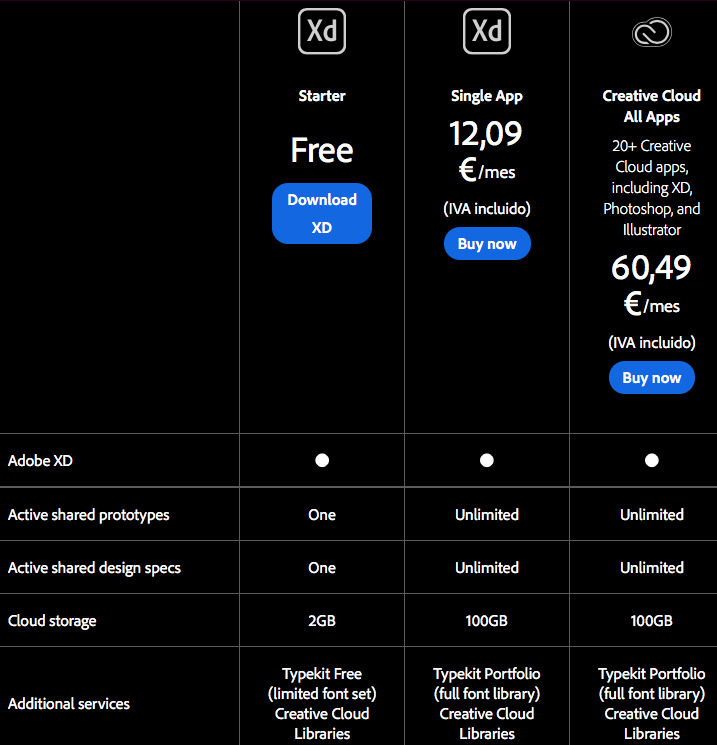
\includegraphics[scale=0.45]{figures/adobe-pricing.png}
\caption{Tarifas de la herramienta de diseño \textit{Adobe Xd}.
\label{fig:adobe_pricing}}
\end{figure}

\subsection{Costes de recursos humanos}
Al ser el equipo de desarrollo de un sólo integrante, no era necesario cumplir con un horario regular, así que para estimar las horas empleadas en el proyecto vamos a asumir que se le dedicaron unas 80 horas mensuales desde Marzo hasta Agosto, ambos inclusive. Además se realizaron 10 reuniones con el director de proyecto, cada una de las cuales, de una duración aproximada de 2 horas. Este último, también cumplía las funciones de consultor y analista así que habrá que tenerlas en cuenta.
\begin{table}[bt]
\begin{center}
\small
\begin{tabular}{|l|c|c|c|}
\hline 
Recurso & Salario (euros/hora) & Horas empleadas & Coste (euros) \\
\hline \hline
Jefe de proyecto & 60 & 20 & 1.200 \\ \hline
Analista & 40 & 90 & 2.000 \\ \hline
Programador & 30 & 400 & 15.200 \\ \hline
\end{tabular}
\caption{Precios estimados de los recursos humanos empleados en el proyecto.}
\label{precios:rrhh}
\end{center}
\end{table}







\chapter{Arquitectura}\label{diseno}
En este capítulo se explicará la arquitectura general del sistema y sus componentes principales: el servicio de localización, el servicio \textit{Backend} y la aplicación \textit{iOS}.

\section{Arquitectura general del sistema}

\begin{figure}[tbp]
\centering
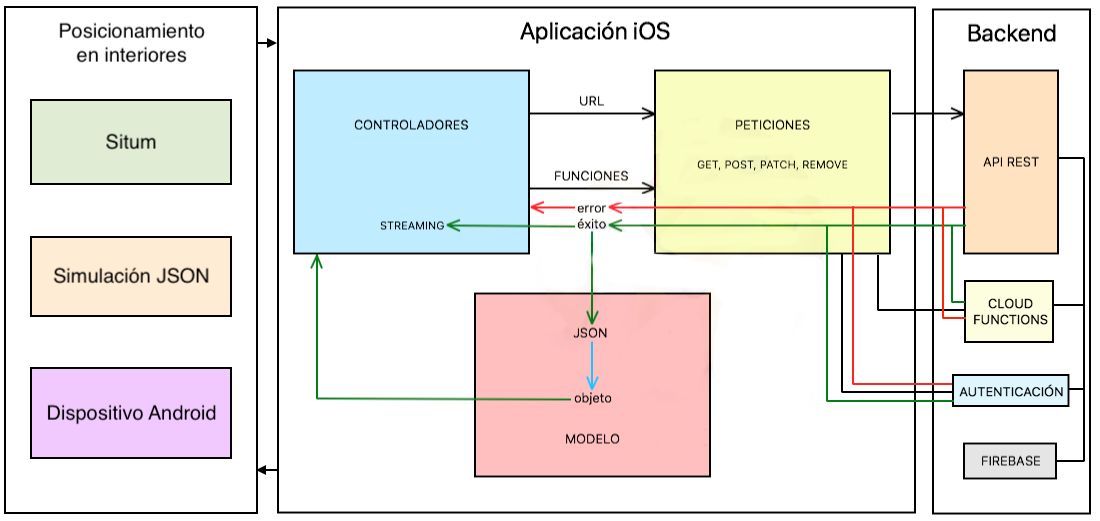
\includegraphics[width=\textwidth]{figures/arquitectura.png}
\caption{Arquitectura general de nuestro sistema de publicidad geolocalizada.\label{fig:arquitectura_2}}
\end{figure}

El sistema está compuesto de tres módulos principales (figura~\ref{fig:arquitectura_2}).
\begin{enumerate}
\item \textbf{\textit{Backend}.} Se ha utilizado la plataforma \textit{Firebase} para desarrollar este módulo. Utilizando los servicios de base de datos en tiempo real, autenticación y \textit{Cloud Functions}.

\item \textbf{Geolocalización.} Es el módulo encargado de determinar la posición del teléfono móvil (y por tanto del usuario)tanto en interiores como en exteriores.

\item \textbf{\textit{Frontend}.} Aplicación \textit{iOS} que se comunica con los otros dos módulos y que permite al usuario interaccionar con la plataforma. 
Se han definido diferentes roles para tener acceso a las distintas acciones previstas en cada caso.
\end{enumerate}

\section{Servicio de localización}
Como se puede observar en la figura~\ref{fig:arquitectura}, el servicio de localización determina la posición del teléfono móvil a partir de los datos que ésta le manda.
Los datos que necesita son el GPS (para la posición en el exterior), los sensores inerciales (acelerómetro, giróscopo y magnetómetro), la información de \emph{Bluetooth} (típicamente balizas fijadas en el edificio) y los datos sobre las redes Wifi detectadas. 
La información sobre la posición se envía directamente a la aplicación \emph{iOS}.

En nuestro prototipo hemos empleado la tecnología de \textit{Situm}.
Se integra su librería en la propia aplicación, y una vez autenticada mediante un código, ella ya se encarga de obtener la información de los servidores de \emph{Situm} (mapas, calibraciones, etc) y de ir obteniendo la información de los sensores y calculando la posición del móvil.


\begin{figure}[tbp]
\centering
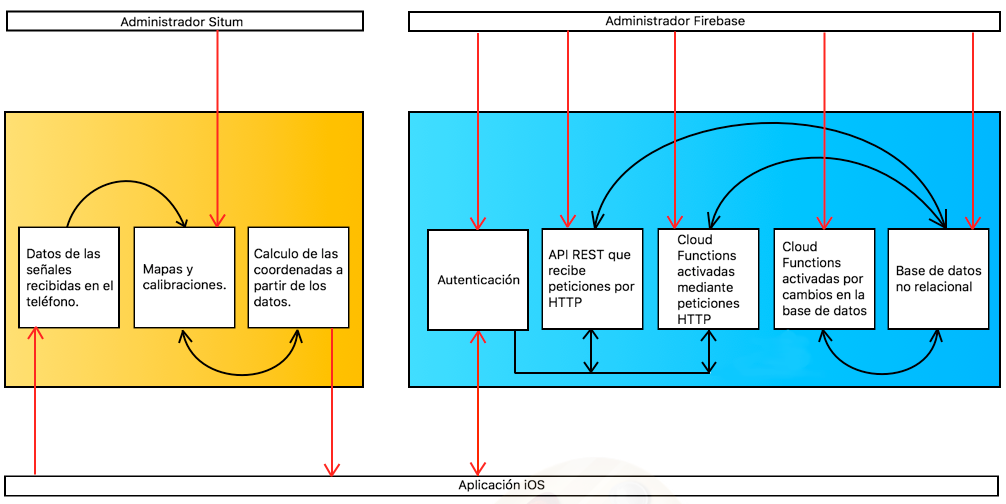
\includegraphics[width=\textwidth]{figures/Untitled2.png}
\caption{Arquitectura general de nuestro sistema de publicidad geolocalizada.\label{fig:arquitectura}}
\end{figure}

El administrador de la plataforma es el único que tiene acceso a la cuenta de \textit{Situm}, de tal manera que debe ser él el que suba las calibraciones y los mapas. Esto puede ser un problema, ya que cada vez que un gestor de centro comercial quiera subir sus mapas o calibraciones tendrá que pasar por el administrador de la plataforma. Quizás en el futuro, los de \textit{Situm} creen una funcionalidad que permita subir mapas y calibraciones a una cuenta, sin necesidad de ser propietarios de la misma.



\subsection{Simulación\label{sec:simul_subsec}}

La tecnología de la localización en interiores en el sistema operativo \emph{iOS} es un tema delicado, porque desde hace ya varios años, \emph{Apple} no da acceso a la información de la Wifi. De esa manera, la tecnología de \emph{Situm} para \emph{iOS} depende exclusivamente de la información de las balizas \emph{Bluetooth} fijadas en el entorno.

En nuestro caso, no teníamos a nuestra disposición ningún edificio calibrado con balizas. Y debido al coste y a las complicaciones del despliegue (robos, etc.) no nos planteamos calibrar ningún edificio por nuestros propios medios.

Por lo tanto, hemos pensado en desarrollar otras alternativas (ver figura~\ref{fig:arquitectura}) para probar el prototipo del sistema. 
La primera opción era desarrollar una aplicación Android (ejecutándose en un dispositivo Android) que ``acompañase'' al usuario con móvil \emph{iOS}. De esta forma, se podrían usar cualquier tipo de edificio con Wifis, por ejemplo la propia Facultad de Informática. 
Al final se descartó por ser poco operativo.

La segunda opción era simular el movimiento del propio móvil.
Las ventajas era la sencillez y la facilidad de uso.
Por desgracia, en \emph{iOS} no se puede simular la información de posición. Además, \emph{Situm} aún no tenía finalizada esta característica en su librería, por lo tuvimos que interaccionar con ellos para implementarla en nuestra aplicación.

Se escogió utilizar un fichero JSON con coordenadas que representaban las distintas posiciones de un usuario a lo largo de una ruta por un centro comercial. Este método era el más sencillo, sobre todo porque podíamos trabajar y hacer pruebas sin necesidad de levantarnos de la silla.


\section{Servicio de \textit{Backend}}
En esta sección se hablará sobre los servicios de la plataforma \textit{Firebase} que fueron utilizados a lo largo de la realización de este proyecto; autenticación, \textit{API REST}, \textit{Cloud Functions} y sus implicaciones sobre el modelo de datos.

\subsection{Autenticación}
Podemos observar en la figura~\ref{fig:arquitectura} que para comunicarnos con \textit{Firebase}, la aplicación debe pasar primero siempre por un proceso de autenticación. Como hemos utilizado la \textit{API REST}, debíamos añadir a toda \textit{URL} la \textit{query-string} \textbf{\textit{key=[API\_KEY]} }\cite{noauthor_firebase_nodate-1}. Este \textit{API\_KEY} es un \textit{token} que se le proporciona al usuario cuando inicia sesión mediante alguno de los múltiples métodos soportados: \textit{Google}, \textit{Twitter}, \textit{Facebook} u otros \cite{noauthor_users_nodate}.

También será necesario ajustar las reglas de \textit{Firebase} a nuestro gusto. Dependiendo de si sólo se quieren permitir las lecturas y las escrituras a usuarios autenticados (ver código~\ref{list:rules-auth}), o si por motivos de comodidad o para realizar alguna prueba, nos interesa desactivar la autenticación y permitir lecturas y escrituras a cualquiera (ver código~\ref{list:rules-true}). Pero las reglas de \textit{Firebase} permiten hacer muchas más cosas, hay una amplia documentación al respecto \cite{noauthor_firebase_nodate}.

\begin{lstlisting}[language=json,style=interfaces,caption=Reglas Firebase que exigen estar autenticado para hacer cambios.,label={list:rules-auth}]
{
  "rules":
  {
    ".read": "auth != null",
    ".write": "auth != null"
  }
}
\end{lstlisting}

\begin{lstlisting}[language=json,style=interfaces,caption=Reglas Firebase que permiten leer y escribir a cualquier usuario.,label={list:rules-true}]
{
  "rules":
  {
    ".read": true,
    ".write": true
  }
}
\end{lstlisting}

\subsection{\textit{API REST}}
Para acceder a los datos se ha decidido utilizar una \textit{API REST}, debido a que este método soporta todas las funcionalidades necesarias para el desarrollo del proyecto y además es uno de los más extendidos. De modo que, al igual que con los servicios de localización, aquí tenemos otra caja negra que nos permitirá adaptarnos fácilmente el día que decidamos cambiar de servidores.

Como se aprecia en la figura \ref{fig:arquitectura}, este componente del sistema recibe una petición del usuario autenticado, escribe y/o lee de la base de datos y finalmente devuelve una respuesta a dicho usuario.

\subsection{\textit{Cloud Functions}}\label{cloud:section}
En esta sección comentaremos los dos tipos de \textit{Cloud Functions} utilizadas y sus diferencias a la hora de integrarse con el resto de componentes de la plataforma.

\subsubsection*{\textit{Cloud Functions} activadas mediante peticiones \textit{HTTP}}
Estas funciones tienen asociada una \textit{URL}, se ejecutan mediante una petición \textit{HTTP} de un usuario autenticado. Leen y/o escriben la base de datos y pueden devolver una respuesta a dicho usuario, como muestra el esquema \ref{fig:arquitectura}.

Para cambiar \textit{Firebase} por otra plataforma o por nuestros propios servidores, el único cambio que habría que hacer en la aplicación \textit{iOS} sería la \textit{URL}.

\subsubsection*{\textit{Cloud Functions} activadas tras cambios en la base de datos}
Estas funciones se ejecutan sin intervención del usuario, se vinculan con un determinado nodo de la base de datos de manera que se lanzan cuando se produce un cambio en el mismo (esquema de la figura~\ref{fig:arquitectura}). Estarían aisladas de los demás componentes del proyecto, si un día quisieramos cambiar de servidores, añadir, eliminar o modificar alguna de estas funciones en caliente, no habría que tocar en absoluto la aplicación \textit{iOS}.

\subsection{Modelo de datos}
Al ser una base de datos no relacional en formato \textit{JSON}, nos quedaría una estructura de árbol con varios niveles (ver código~\ref{list:tree-nosql}). Si tratásemos de hacer lo mismo con un modelo relacional nos quedaría un esquema como el de la figura~\ref{fig:modelo}.

\begin{lstlisting}[language=json,style=interfaces,caption=Árbol formado por una base de datos no relacional.,label={list:tree-nosql}]
"Buildings" : {
  "3598" : {
  	"Managers" : {
  		"-4712897510522395898" : {
  			"Email" : "gestor.centro.comercial@gmail.com"
		}
  	},
  	"Shops" : {
  		"-LKnOeINwIY7m0wEfK90" : {
  			"Name" : "Cafeteria",
  			"Offers" : {
  				"-LKnTA635eXVIBDOxQpt" : {
  					"Description" : "Croissant, zumo y Colacao",
  					"Floor" : 1,
  					"Latitude" : 43.3328167533505,
  					"Longitude" : -8.411021903157234,
  					"Radius" : 20,
  					"Title" : "Desayuno 2 euros",
  					"expiration" : "1535494759171.4001",
  					"quantity" : "10"
				}
  			}
  		}
  	}
}
\end{lstlisting}

\begin{figure}[tbp]
\centering
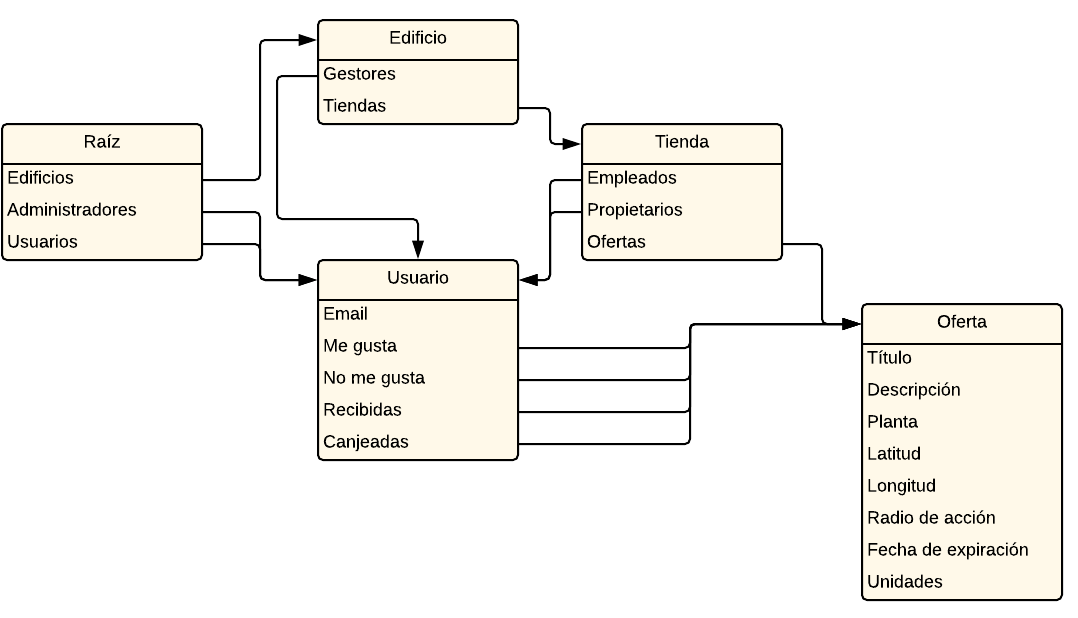
\includegraphics[scale=0.35]{figures/modelo.png}
\caption{Modelo de datos del servicio \emph{Backend}.
 Por comodidad, se representa el modelo de una base de datos relacional equivalente.\label{fig:modelo}}
\end{figure}

\subsubsection*{Limitaciones de una base de datos \textit{NoSQL}} \label{nosql}
Una base de datos no relacional, no se estructura de la misma manera que una que sí lo es (figura~\ref{fig:nosqlVS}). Por ejemplo, en esta aplicación tenemos las ofertas, que se encuentran dentro de una tienda y que a su vez se encuentran dentro de un edificio. Pero cuando un usuario indica que le gusta una oferta, la información se guarda en su perfil, no en la oferta. Surge aquí un problema, porque quizás queramos datos que ya están almacenados en el propio nodo de la oferta, pero los queremos accesibles desde el nodo del usuario.

Este proyecto nació con la idea de utilizar solamente el servicio de base de datos de \textit{Firebase}, así que en situaciones como estas no hubo más opciones que replicar datos. Lo cual es muy ineficiente, siendo la otra opción almacenar la \textit{URL} de la oferta en el nodo del usuario y realizar una petición extra, pero esto aumentaría el consumo de datos en el teléfono móvil de los usuarios.

\subsubsection*{Aparición de \textit{Cloud Functions}}
Poco a poco fueron apareciendo nuevas necesidades en el proyecto, que obligaron a utilizar \textit{Cloud Functions}. La capacidad de ejecutar código en un servidor permite cambiar por completo la arquitectura de una base de datos de este tipo. Ya que para solucionar el problema anteriormente comentado de los \textit{me gusta}, el usuario solamente con una petición podría bajarse las ofertas de la tienda ya con su información personal. Sin necesidad de replicar datos ni de hacer varias peticiones, la función de \textit{Cloud Functions} recibiría la petición, realizaría las búsquedas pertinentes en la base de datos, compondría el listado de ofertas con datos del usuario y se la devolvería al cliente.

\begin{figure}[tbp]
\centering
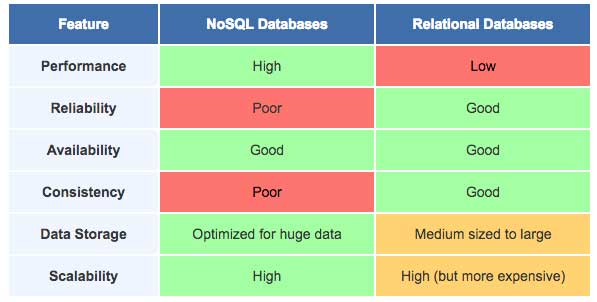
\includegraphics[scale=0.5]{figures/nosqlVS.jpg}
\caption{Relacional VS No relacional.\label{fig:nosqlVS}}
\end{figure}

\section{Arquitectura de la aplicación móvil: MVC}
Para el desarrollo de la aplicación \textit{iOS} se ha utilizado el patrón Modelo Vista Controlador. La herramienta \textit{Xcode}, nos permite crear aplicaciones \textit{iOS} mediante este patrón de diseño.
En la figura~\ref{fig:arq_ios} se puede ver la arquitectura de la aplicación \emph{iOS}. A continuación, explicaremos cada uno de los elementos: modelo (datos y peticiones), vista y controlador. 

\begin{figure}[tb]
\centering
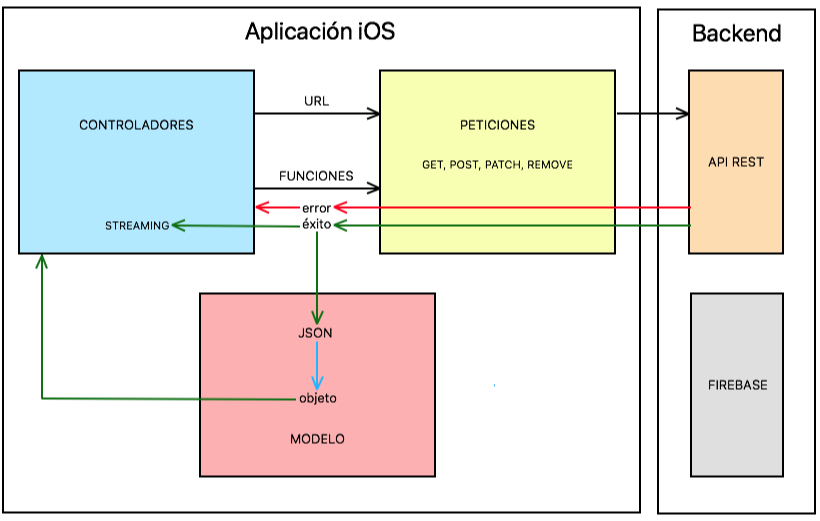
\includegraphics[width=0.89\textwidth]{figures/esquema-impl.png}
\caption{Arquitectura general de la aplicación \emph{iOS}.\label{fig:arq_ios}}
\end{figure}

\subsection{Modelo}
En esta subsección hablaremos de como se organiza la aplicación para obtener los datos de \textit{Firebase}.

\paragraph{Peticiones.}
Se separan del resto del código, las funciones utilizadas para comunicarse con la base de datos. Por ejemplo, si queremos pedir una oferta determinada, simplemente ejecutamos la función correspondiente, la cual nos devolverá dicha oferta. Las peticiones se organizan en clases (figura~\ref{fig:peticiones}) y cada función se define como un método estático, de esta manera pueden ser llamadas desde cualquier otra clase sin necesidad de crear una instancia, esto ofrece varias ventajas.

\begin{itemize}
\item{}\textbf{Reutilización de código.} Una petición, por ejemplo para obtener una oferta determinada, es probable que se vaya a llamar desde multitud de clases.

\item{}\textbf{Modificaciones y errores.} Si una petición no está funcionando como se esperaba o queremos modificar algo. Será mucho más fácil arreglar el problema si la tenemos aislada y localizada, evitándonos buscar todas las veces que se hace la petición por todo el código.
\end{itemize}

\subsubsection*{Programación orientada a objetos}
Todos los nodos que recuperemos de la base de datos deberán mapearse en clases para poder así trabajar con ellos. El modelo de datos de la figura~\ref{fig:modelo}, daría lugar a las clases que vemos en la figura~\ref{fig:objetos}.

\begin{figure}[tbp]
\centering
\subfigure{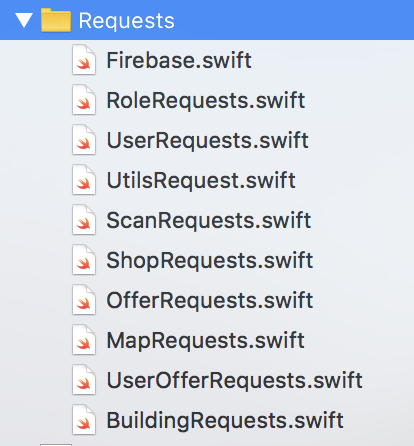
\includegraphics[scale=0.6]{figures/peticiones.png}\label{fig:peticiones}}
\subfigure{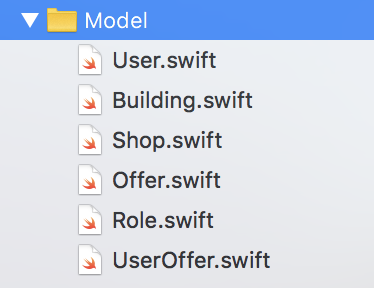
\includegraphics[scale=0.6]{figures/objetos.png}\label{fig:objetos}}
\caption{Modelo \textit{app}: (a) Aislamiento de peticiones y (b) clases de la aplicación.}
\end{figure}

\subsection{Vista}

\begin{figure}[t]
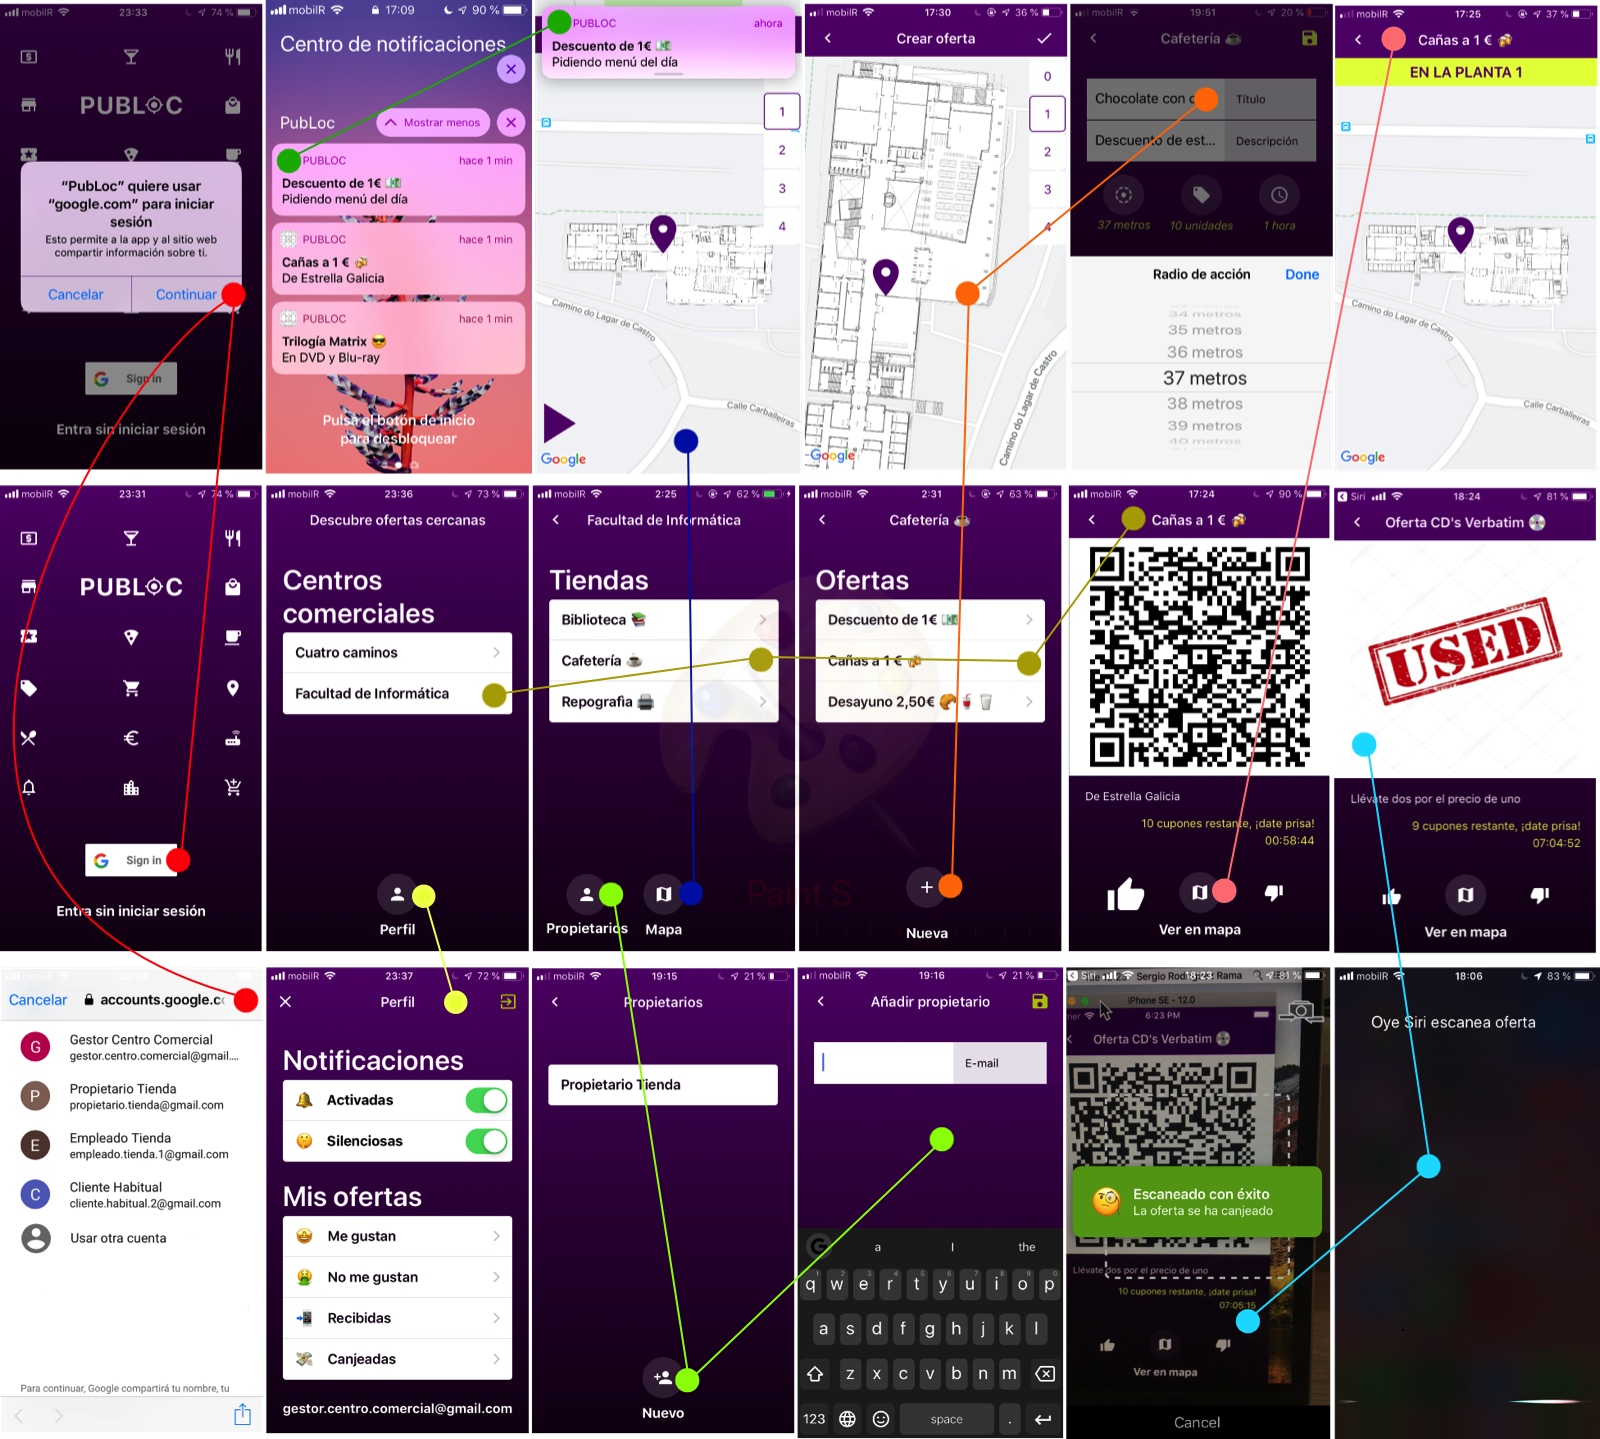
\includegraphics[width=\textwidth]{figures/esquema2.png}
\captionsetup{singlelinecheck=off,font=footnotesize}
\caption[Conjunto de las vistas diseñadas en la aplicación \emph{iOS} agrupadas por temática.]{Conjunto de las vistas diseñadas en la aplicación \emph{iOS} agrupadas por temática:
\legendbox{mi_rojo} Autenticación,
\legendbox{mi_dorado} Datos generales (centros comerciales, tiendas y ofertas), 
\legendbox{mi_verde} Notificaciones,
\legendbox{mi_azul_oscuro} Mapa de edificio, 
\legendbox{mi_naranja} Nueva oferta,
\legendbox{mi_rosa_pastel} Mapa de oferta,
\legendbox{mi_amarillo_claro} Perfil,
\legendbox{mi_verde_claro} Crear rol,
\legendbox{mi_celeste} Escaneo de códigos \textit{QR}.\label{fig:esquema2}}
\end{figure}

En la figura~\ref{fig:esquema2} podemos ver como se ha estructurado la vista de la aplicación, las diferentes pantallas y como se relacionan entre ellas.

\paragraph{Autenticación.} Pantalla incial de la aplicación, con dos botones. Uno para iniciar sesión con \textit{Google} y otro para entrar a la aplicación directamente. Si seleccionamos iniciar sesión con \textit{Google} se nos redirigirá automáticamente al selector de cuentas y cuando se termine la autenticación, podremos visualizar los centros comerciales.

\paragraph{Datos generales.} Estas pantallas contienen los listados de centros comerciales, tiendas y ofertas, hasta llegar al detalle de la oferta donde se encuentra el código \textit{QR}. Dependiendo de los roles que tenga el usuario, las acciones \textit{CRUD} de roles, ofertas y tiendas le serán visibles o no.

\paragraph{Notificaciones.} Cuando el usuario entra en el radio de acción de una oferta, salta una notificación y se puede visualizar tanto con la \textit{app} abierta como con el móvil bloqueado, en la parrilla de notificaciones.

\paragraph{Mapa de edificio.} Desde la pantalla que contiene las tiendas de un centro comercial, podemos ver su mapa. Desde él, veremos nuestra posición en el plano, pudiendo seleccionar cualquiera de las plantas que tiene el edificio para ver las ofertas que hay en ella.

\paragraph{Nueva oferta.} Desde la pantalla que contiene las ofertas de una tienda, podemos añadir una nueva oferta. Tendríamos que darle un nombre, una descripción, un radio de acción, una duración y un límite de unidades disponibles. Es necesario tener rol de propietario de dicha tienda para poder llevar a cabo esta acción.
Las pantallas de creación de tienda no aparecen en el esquema porque sería muy similar a éstas, la única diferencia es que el único atributo de las tiendas es su nombre.

\paragraph{Mapa de oferta.} Desde la pantalla de detalle de una oferta, podemos ver su posición en el mapa. Se mostrará la planta del edificio que la contiene y no habrá botones que nos permitan explorar las demás.

\paragraph{Perfil.} Aquí se pueden silenciar o desactivar las notificaciones y también ver las ofertas del usuario: favoritas, rechazadas, recibidas y canjeadas. Si seleccionamos cualquiera de estas, se mostrará una lista de ofertas similar a la que mostrábamos al seleccionar una tienda.

\paragraph{Crear rol.} Las pantallas de creación de rol son idénticas para cualquier rol que creamos crear, simplemente será necesario introducir el \textit{email} de un usuario autenticado en la plataforma para asignarle el rol en cuestión. Estas funcionalidades no estarán visibles para todos los usuarios de la aplicación, sólo para aquellos que tengan los permisos necesarios.

\paragraph{Escaneo de códigos \textit{QR}.} El escáner de códigos \textit{QR} puede lanzarse desde un botón que hay en perfil de usuario, pero también se puede abrir utilizando atajos de \textit{Siri} y funciona aunque la aplicación esté cerrada. Cuando se realiza un escaneo, se proporciona siempre \textit{feedback} al empleado de la tienda, mostrándole un aviso por pantalla.

\subsubsection*{Sinergia entre el modelo y la vista}
Aunque el modelo y la vista están separados según el patrón Modelo-Vista-Controlador, puede pasar que la propia estructura de la base de datos condicione la interfaz de usuario. Como vimos en la sección  \ref{nosql}, hay una separación entre datos de perfil y datos generales de la aplicación. Un ejemplo de como podría afectar esta arquitectura a la interfaz de usuario sería el siguiente:

Imaginemos que se quiere que los botones \textit{like}/\textit{dislike}  vayan incorporados en las celdas de la tabla de ofertas de una tienda. Como este proyecto nació con la idea de utilizar la base de datos que ofrece \textit{Firebase} únicamente, comunicándonos con ella mediante \textit{API REST}; para lograr esto, a la hora de elaborar la tabla deberíamos tener acceso a las ofertas de la tienda y a las ofertas del usuario para compararlas y saber que opinión tiene el usuario al respecto de cada una de ellas. Esto no solamente obligaría a hacer una petición extra, sino que también obligaría al terminal móvil del cliente a trabajar de más: almacenando dos listas de ofertas en lugar de una, comparándolas y creando una a partir de ambas.

Para darle solución a este problema, se decidió poner los botones de \textit{like}/\textit{dislike} situados en el detalle de la oferta, en lugar de tenerlos en cada celda de la tabla. De esta manera sólo se descargaría la información de usuario de una oferta determinada cada vez que entramos en ella, en lugar de tener que pedirlas todas para filtrar las ofertas de la tienda.

Más tarde, surgió la necesidad de incluir \textit{Cloud Functions} en el proyecto y apareció la posibilidad de incluir los botones en las celdas, pero se decidió no abordar este cambio de diseño por falta de tiempo y dejarlo para futuras iteraciones.

\subsection{Controlador}
El controlador funciona como intermediario entre la vista y el modelo, cambios en el modelo que tendrán su efecto en la vista y acciones en la vista que tendrán su efecto en el modelo, serán gestionados por el controlador. Las aplicaciones \textit{iOS} se construyen basándose en el patrón Modelo-Vista-Controlador, a continuación explicaremos como se estructuran los diversos controladores que componen una aplicación.

\subsubsection*{Controlador padre}
No es obligatorio, pero es recomendable comenzar toda aplicación \textit{iOS} con un controlador padre, conocido como \textit{UINavigationController}. Tendrá una pila en la cual se irán añadiendo controladores hijos y él será el encargado de gestionar las transiciones entre ellos y la navegación a través de las diversas pantallas de la aplicación.

\paragraph{\textit{Push}.} Consiste en añadir un nuevo controlador hijo a la pila, el cual se convertirá en el controlador visible (el que verá y con el interactuará el usuario). Si se animase la transición, la nueva pantalla aparece en escena por defecto deslizándose de derecha a izquierda (en árabe, de izquierda a derecha).

\paragraph{\textit{Pop}.} Consiste en sacar de la pila el último controlador hijo añadido, convirtiéndose el siguiente de la pila en el controlador visible. Esta acción es más conocida como \textit{Atrás} y suele representarse con un botón con una flecha en la parte superior izquierda (en árabe, la derecha). También suele realizarse esta acción deslizando el dedo en la dirección contraria al \textit{push} desde el borde de la pantalla, ver figura~\ref{ref:pop-push}.

\begin{figure}[tbp]
\centering
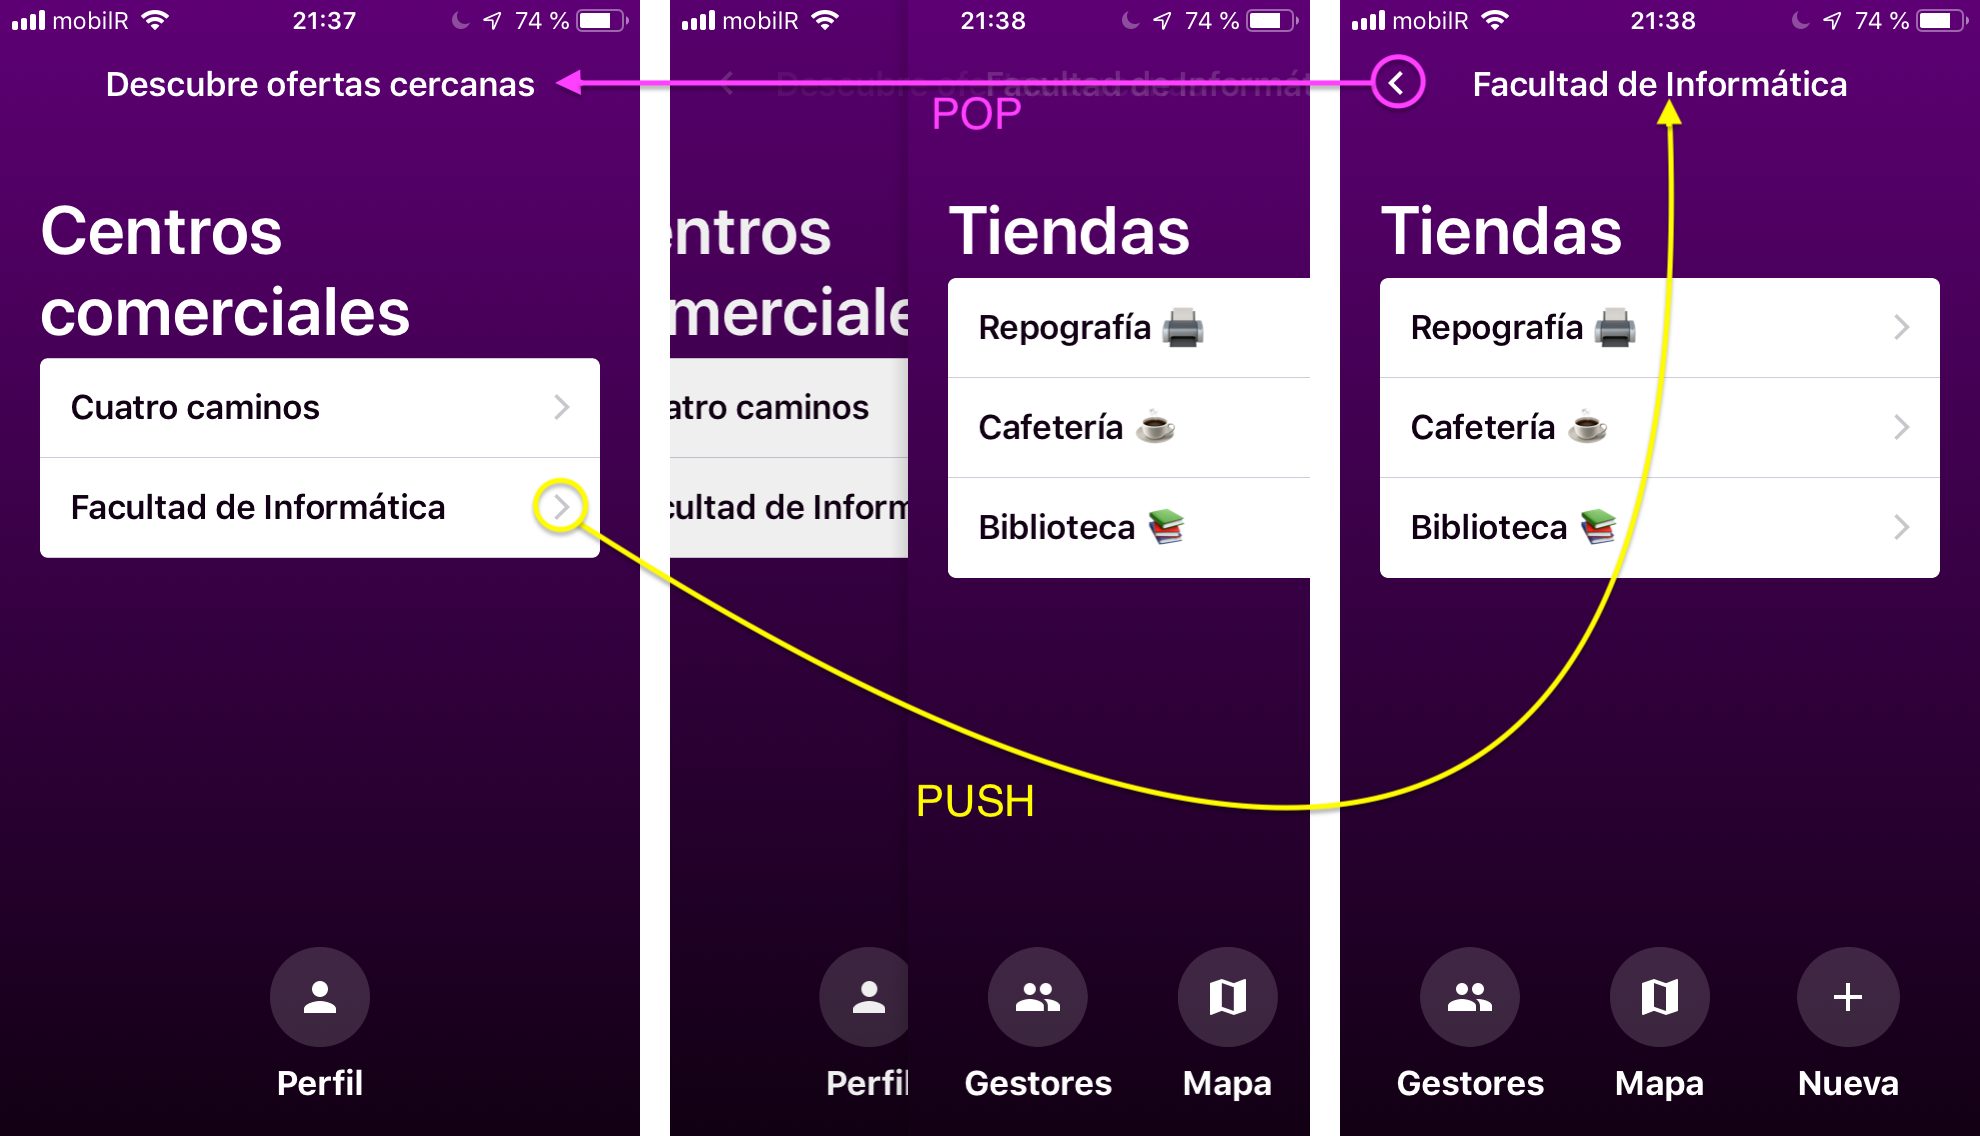
\includegraphics[scale=0.15]{figures/pop-push.png}
\caption{Transiciones entre controladores: \textit{push} y \textit{pop}.\label{ref:pop-push}}
\end{figure}

\subsubsection*{Controladores hijos}\label{contr-hijos}
Serían todos aquellos que no son el \textit{UINavigationController}. Todo controlador tiene asociada una vista, es el controlador quien maneja todas las interactuaciones del usuario con la vista y también es él quien se encarga de mostrarle al usuario a través de la vista todo lo que sea necesario. Una característica que tiene un controlador, es que tiene la capacidad de presentar en pantalla a cualquier otro. Pero a diferencia que con el \textit{UINavigationController}, no va metiendo los nuevos controladores que presenta en una pila, sino que simplemente los muestra y ahí permanecen hasta que se cierran.

Un ejemplo de esto serían las alertas, que también son controladores independientes; presentados por otro controlador que no tiene porque ser un \textit{UINavigationController}, ver figura~\ref{fig:modal}.

\begin{figure}[t]
\centering
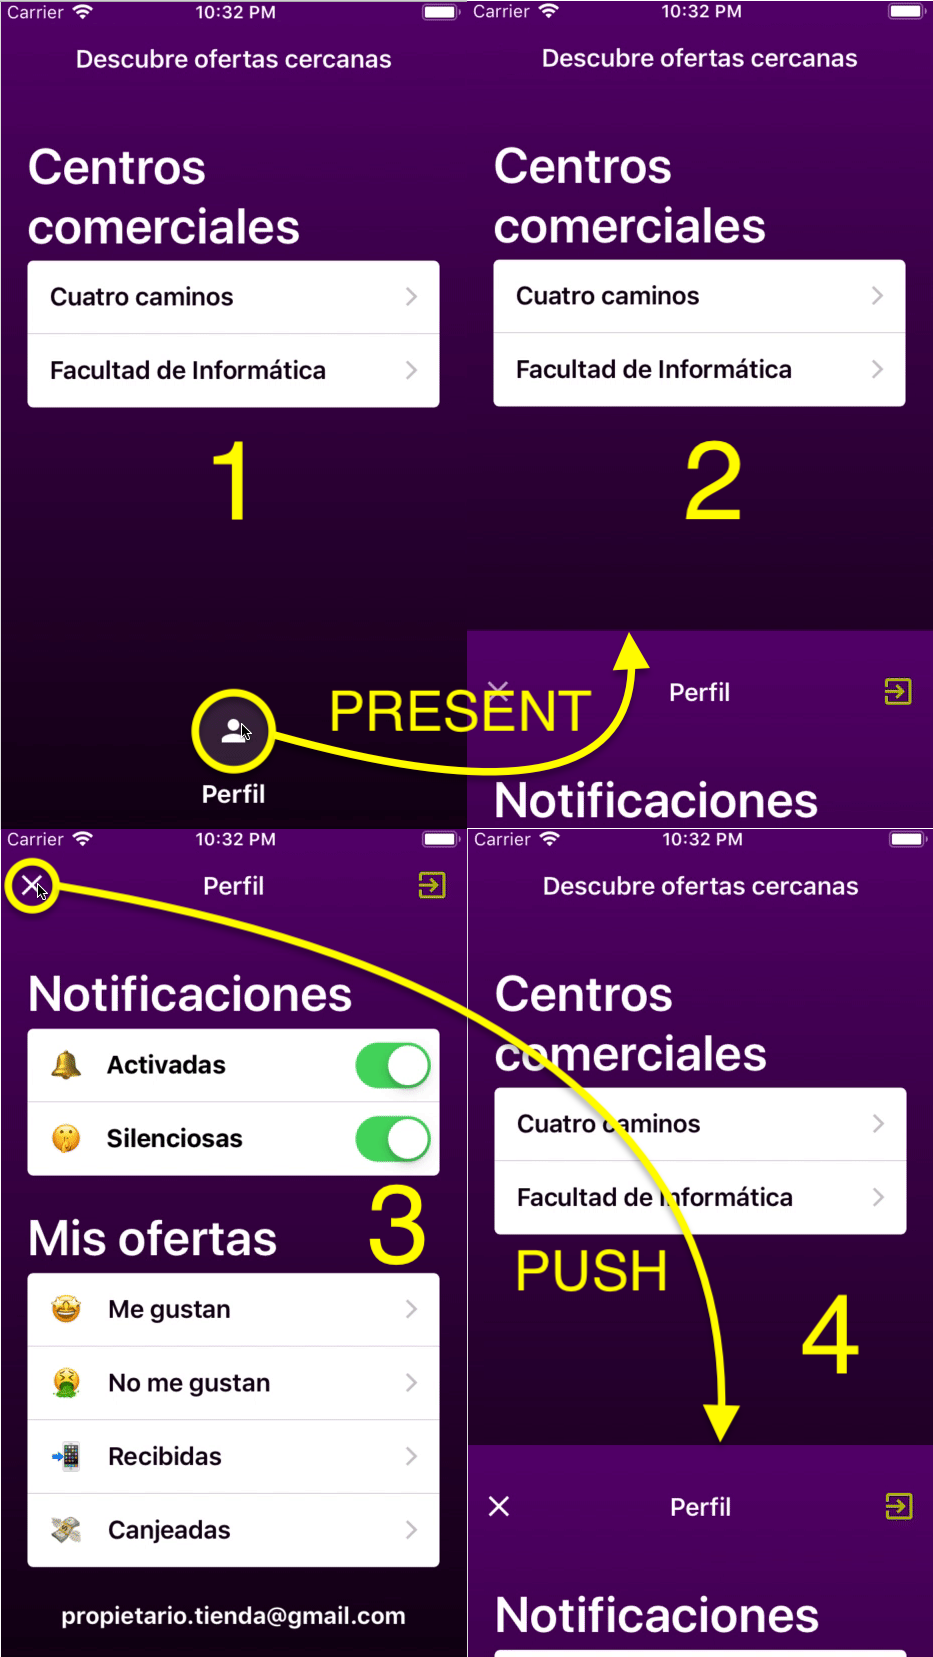
\includegraphics[scale=0.22]{figures/modal.png}
\caption{\textit{Present} para mostrar en pantalla un controlador y \textit{dismiss} para quitarlo.\label{fig:modal}}
\end{figure}

\subsubsection*{Un \textit{UINavigationController} puede ser presentado por otro controlador}
Un controlador normal de los que comentábamos en el apartado \ref{contr-hijos} puede presentar a un controlador padre para que empiece a formar una nueva pila. Puede haber más de un \textit{UINavigationController} y por lo tanto, más de una pila de controladores a la vez, pero sólo uno visible.


\chapter{Implementación}

En este capítulo se comenta cómo el diseño fue llevado a la práctica.
Empezaremos explicando la integración el servicio de localización, a continuación la implementación del servicio de \textit{Backend}, y por último, el  desarrollo de la aplicación móvil.

% Servicio de localización
\section{Servicio de localización}
Para integrar los servicios de \textit{Situm} en una aplicación \textit{iOS} hay que seguir los siguientes pasos \cite{noauthor_situm_nodate}.

\begin{enumerate}
\item \textbf{Crear una cuenta de \textit{Situm Dashboard}.} Así podremos empezar a subir planos de edificios y calibraciones \cite{noauthor_situm_nodate} a nuestro perfil. 

\item \textbf{Subir planos de un edificio.}\label{item:calib~.aciones} Hay que subir los planos de cada planta. Se debe situar el plano correctamente sobre un mapa de \textit{Google}. Una vez subido el primero, los siguientes se situarán sobre el mapa de la misma manera: mismas coordenadas, altura y orientación. Por eso es importante que todos los planos correspondientes a las plantas de un mismo edificio tengan la misma resolución y estén alineados, ver figura~\ref{fig:planos-situm}.

\item{}\textbf{Subir las calibraciones.} Para ello se utilizó la aplicación \textit{Android} que hay disponible en la \textit{Play Store} \cite{noauthor_aplicacion_nodate}. Iniciando sesión con la misma cuenta del \textit{Dashboard} se ``calibra'' el edificio, es decir, moverse por el edificio indicando y, a medida que se avanza, identificar en el mapa que muestra la aplicación cual es nuestra posición.

\item{}\textbf{Añadir las librerías de \textit{Situm} a nuestra aplicación.} Debemos descargar el \textit{framework} \cite{situm_situm_nodate} e incorporarlo a nuestro proyecto de \textit{Xcode}, ver figura~\ref{fig:sdk-xcode}.

\item{}\textbf{Añadir la \textit{API KEY} al proyecto y empezar a trabajar.} Hay tutoriales oficiales de \textit{Situm} sobre como añadir la \textit{API KEY} y empezar a obtener la información sobre los edificios que hay subidos en la cuenta del \textit{Dashboard} \cite{noauthor_situm_nodate}, ver figura~\ref{fig:api-situm-code}.

\begin{figure}[tbp]
\centering
\subfigure{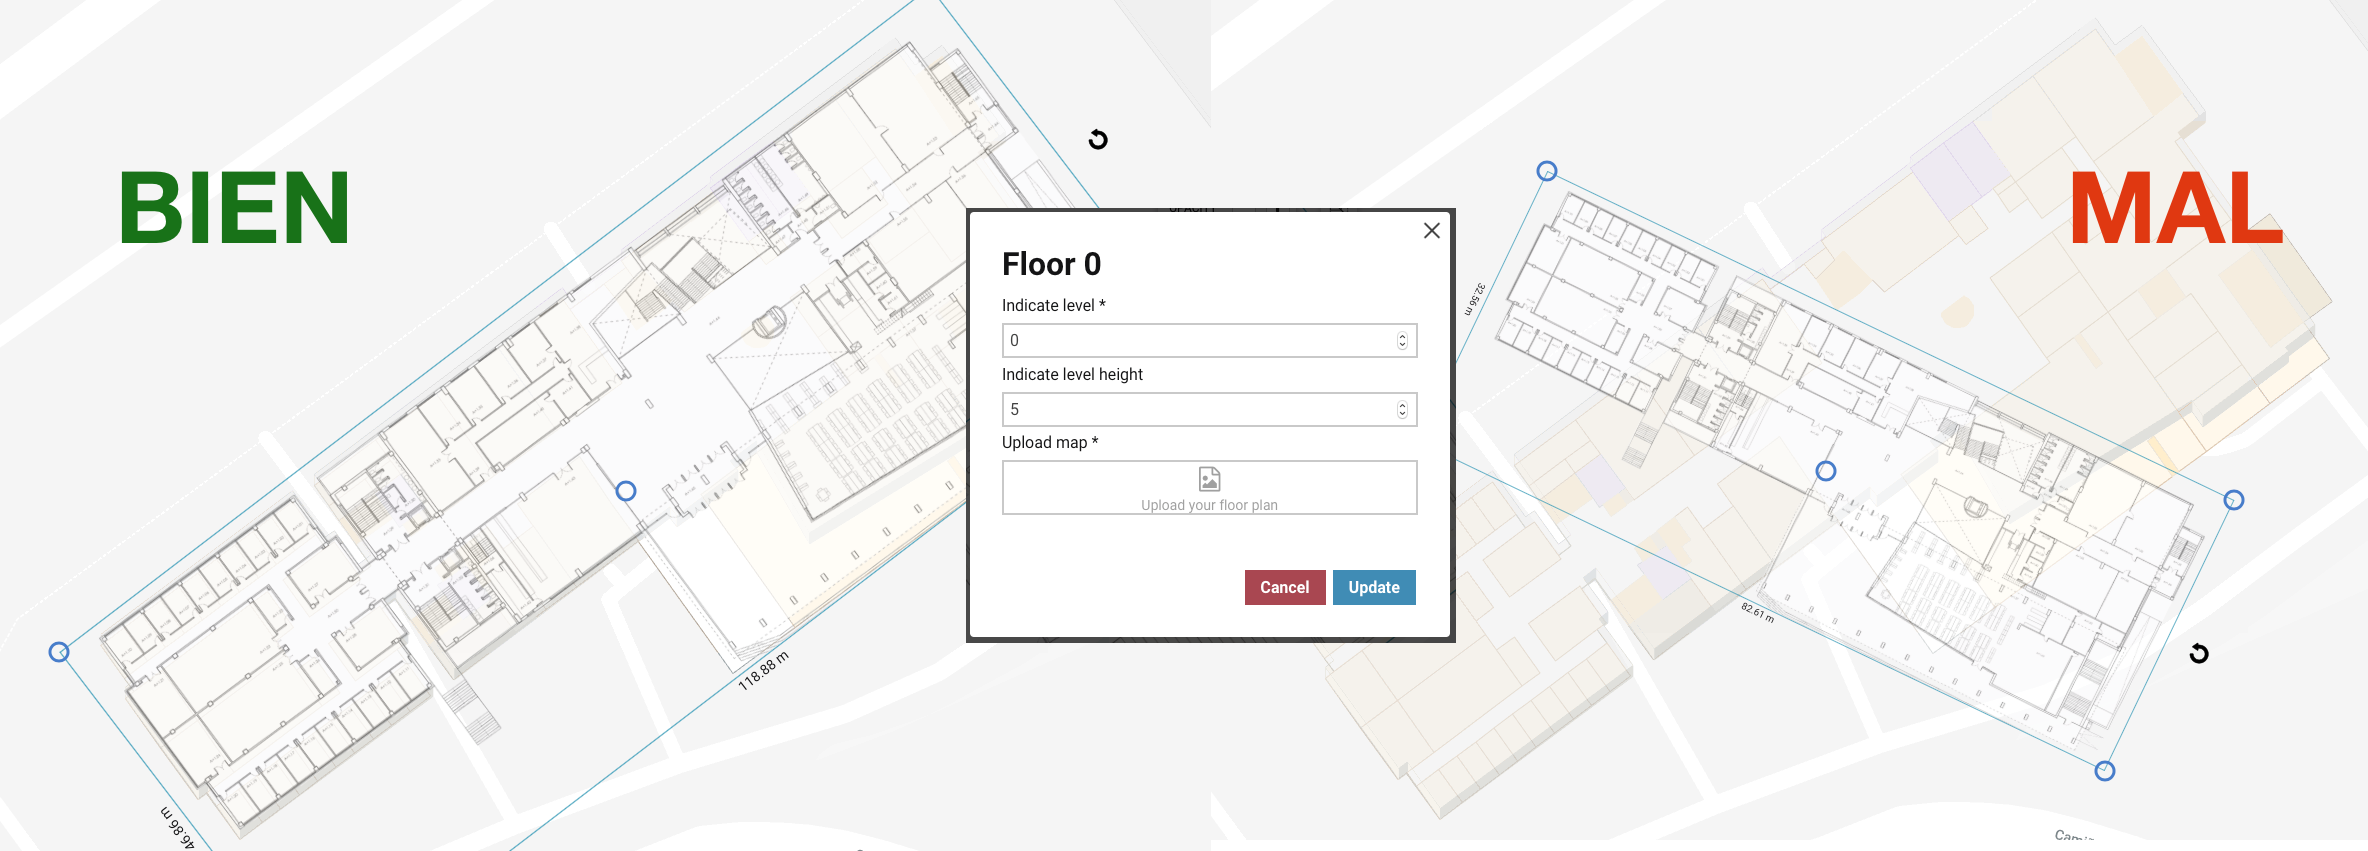
\includegraphics[width=\textwidth]{figures/planos-situm.png}\label{fig:planos-situm}}
\vspace{3ex}
\subfigure{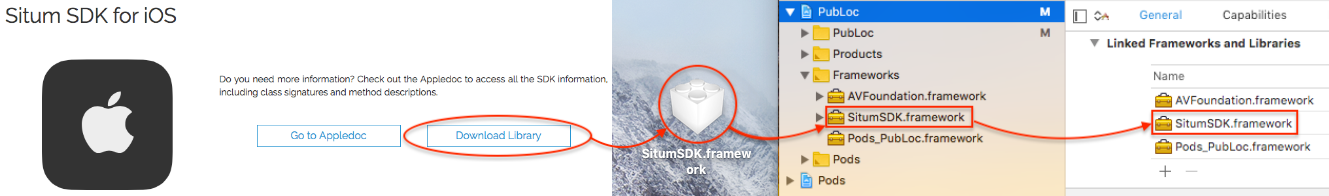
\includegraphics[width=\textwidth]{figures/sdk-xcode.png}\label{fig:api-situm-code}}
\vspace{3ex}
\subfigure{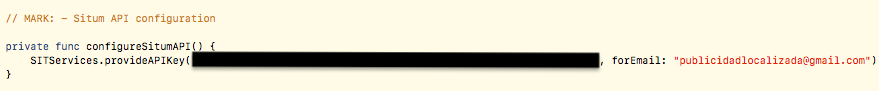
\includegraphics[width=\textwidth]{figures/api-situm-code.png}\label{fig:sdk-xcode}}
\caption[Configuración de la localización de \textit{Situm}.]{Configuración de la localización de \textit{Situm}: (arriba) subir los planos alineado de cada planta; (centro) recoger el \textit{API KEY} en el \textit{Dashboard} y descarga en el directorio de \textit{frameworks} del proyecto; y (abajo) añadir a \textit{Linked Frameworks and Libraries}.}
\end{figure}
\end{enumerate}

\subsection{Simulación con fichero \textit{JSON}}
Para hacer pruebas con la aplicación se decidió utilizar un fichero \textit{JSON}, como se explica en el apartado~\ref{sec:simul_subsec}. El contenido de este fichero es una lista de objetos \textit{JSON} y cada uno de ellos contendría unas coordenadas (longitud y latitud) y la planta del edificio en la que estaría ubicado (ver código \ref{list:json-simul}).

Desde la aplicación, se recorre el fichero en bucle y se va moviendo una chincheta sobre el mapa, saltando de un punto a otro y cambiando de planta cuando sea necesario.
Hay que señalar que se debe animar el movimiento para que no se aprecien los saltos de manera brusca.
El resultado final es idéntico al que veríamos en cualquier aplicación de mapas.

Para crear este fichero usamos una herramienta \textit{online} \cite{noauthor_herramienta_nodate} que genera un \textit{JSON} a partir de una ruta que nosotros mismos diseñamos marcando una sucesión de puntos en un mapa (figura~\ref{fig:sim-json-gen}). Pero la información sobre el piso hubo que metérsela a mano.

\begin{figure}[bt]
\centering
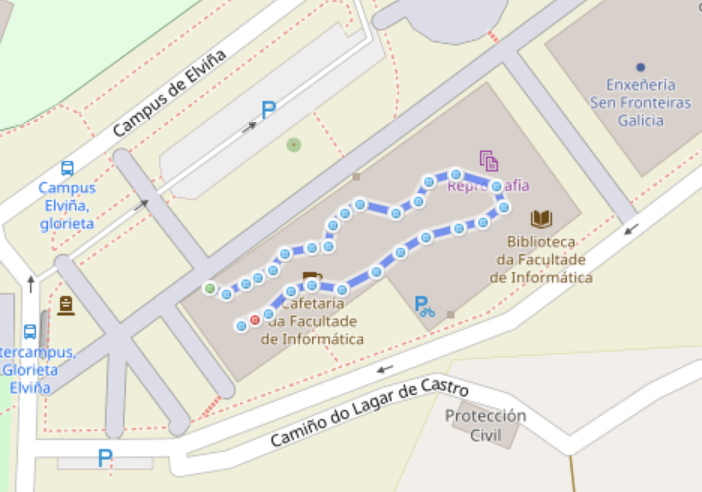
\includegraphics[width=0.6\textwidth]{figures/sim-json-gen.png}
\caption{Creación de ruta exportables a \textit{JSON}.\label{fig:sim-json-gen}}
\end{figure}

\begin{lstlisting}[language=json,style=interfaces,caption={Fragmento de simulación \textit{JSON}, coincide con el cambio del piso 0 al 1.},label={list:json-simul}]
...
{
   "lon": -8.41110706,
   "lat": 43.3329964,
   "lev": 0
}, {
   "lon": -8.41106414,
   "lat": 43.332969,
   "lev": 0
}, {
   "lon": -8.41105341,
   "lat": 43.3329222,
   "lev": 1
}
...
\end{lstlisting}


% Servicio de Backend
\section{Servicio de \textit{Backend}}
En esta sección se comenta  el desarrollo de toda la parte de servidor o \textit{Backend} del proyecto. Empezaremos por la fase de autenticación, la \textit{API REST}, el uso de las \textit{Cloud Functions} y la implementación del modelo de datos.

\subsection{Autenticación}
Cuando un usuario se autentica en la aplicación mediante cualquiera de los métodos ofrecidos por \textit{Firebase}, se le asigna un determinado \textit{token} de usuario, ver figura~\ref{fig:access-token}.

\begin{figure}[bt]
\centering
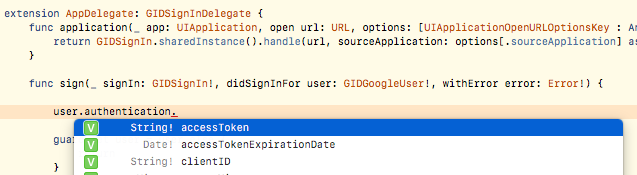
\includegraphics[width=0.8\textwidth]{figures/access-token.png}
\caption{El \textit{token} es un \textit{string} que se puede obtener tras una autenticación exitosa.\label{fig:access-token}}
\end{figure}

Lo único que hay que hacer es añadir ese \textit{token} como una \textit{query-string} a toda \textit{URL} a la que hagamos una petición.

\subsection{\textit{API REST}}
Para comunicarnos a la \textit{API REST} se utilizó la librería \textit{Alamofire} \cite{noauthor_alamofire_nodate}, la cual permite realizar de manera sencilla peticiones \textit{HTTP}. A continuación, hablaremos sobre como se implementó esta importante parte del proyecto.

\subsubsection*{Composición de las \textit{URLs}} \label{comp:url}
Dada la estructura en árbol de una base de datos no relacional, para formar la \textit{URL} hay que ir concatenando al identificador del proyecto las claves de aquellos nodos por los que hay que pasar para llegar al que nos interesa (separados por ``\textit{/}''). Cuando se llega al nodo al que se quiere hacer la petición, se debe concatenar ``\textit{.json}'' a la \textit{URL}. Por ejemplo la \textit{URL} del nodo de la figura~\ref{fig:node} sería: \url{https://publoc-1234.firebaseio.com/Buildings/3598/Shops/-LKnOeINwIY7m0wEfK90/Offers/-LKnSVU1KGgrAuRQymv7.json}

\subsubsection*{Peticiones}
A continuación, se comentan los cuatro tipos de peticiones que se utilizaron.

\paragraph{\textit{GET}.} Petición utilizada para obtener información sobre un nodo de la base de datos. El resultado de la petición es una cadena de texto en formato \textit{JSON} que representa al nodo y cuyos campos se deben \textit{mapear} a un objeto para poder trabajar con él en la aplicación. La \textit{URL} deberá representar al nodo deseado, ver sección~\ref{comp:url}.

\paragraph{\textit{POST}.} Petición utilizada para crear un nuevo nodo en la base de datos. Cuando hacemos una petición de este tipo, debemos enviarle una cadena de texto en formato \textit{JSON} que represente el valor del nodo que queremos crear en el cuerpo de la petición. La respuesta que nos devuelve el servidor es una cadena de texto en formato \textit{JSON} que contiene el identificador del nodo que se acaba de crear. La \textit{URL} deberá representar al nodo en el que se desea insertar al nuevo, ver sección~\ref{comp:url}.

\paragraph{\textit{PATCH}.} petición utilizada para modificar el contenido de un nodo en la base de datos. Cuando hacemos una petición de este tipo, debemos enviarle una cadena de texto en formato \textit{JSON} que represente aquellos campos del nodo que queremos modificar, como cuerpo de la petición. La respuesta que nos llega de servidor es una cadena de texto en formato \textit{JSON} que contiene aquellos campos del nodo que han sido modificados. La \textit{URL} deberá representar al nodo que se quiere modificar, ver sección~\ref{comp:url}.

\paragraph{\textit{REMOVE}.} petición utilizada para eliminar un nodo. Esta petición devuelve simplemente \textit{200 OK} si se realiza correctamente. La \textit{URL} deberá representar al nodo que se quiere borrar.

\subsubsection*{\textit{Stream} de un nodo}

\begin{lstlisting}[style=interfaces,caption=Fragmento de código correspondiente a un \textit{streaming}.,label={list:alamo-stream}]
public static func stream(url: String, completionFailure: @escaping (DataResponse<Any>) -> Void, completionStream: @escaping (Data) -> Void) -> Request {
	return Alamofire.request(url, method: .get, parameters: nil, encoding: JSONEncoding.default, headers: ["Accept": "text/event-stream"]).responseJSON { (response) in
		switch response.result {
		case .success:
			break
		case .failure:
			completionFailure(response)
		}
	}.stream { (data) in
		completionStream(data)
	}
}
\end{lstlisting}

Desde el controlador se puede hacer \textit{streaming} a un nodo de la base de datos para modificar la vista si se produce un cambio en este, haciendo un petición \textit{GET} a un nodo con la cabecera \textbf{``\textit{Accept}''} a \textbf{``\textit{text/event-stream}''}. La librería \textit{Alamofire} facilita esta tarea, ver fragmento de código~\ref{list:alamo-stream}.


\subsection{\textit{Cloud Functions}}
Como se decidió tarde incluir esta tecnología al proyecto, se utilizaron muchas menos \textit{Cloud Functions} de las que se deberían. Si se hubiesen utilizado desde el principio, muchas tareas podrían haberse realizado de una manera más simple. A continuación un par de ejemplos en los que si se usaron este tipo de funciones, de los dos tipos comentados en el apartado  \ref{sec:cloud_functions}.

\subsubsection*{\textit{Cloud functions} activadas por peticiones \textit{HTTP}}
\begin{lstlisting}[style=interfaces,caption=\textit{Cloud Function} activada por petición \textit{HTTP}.,label={list:cloud-http}]
exports.removeOldOffers = functions.https.onRequest((req, res) => {
const timeNow = Date.now();
	const messagesRef = admin.database().ref('/Buildings');
	messagesRef.once('value', (snapshot) => {
		snapshot.forEach((child) => {
			child.ref.child('/Shops').once('value', (snapshot) => {
				snapshot.forEach((child) => {
					child.ref.child('/Offers').once('value', (snapshot) => {
						snapshot.forEach((child) => {
							if (Number(child.val()['expiration']) <= timeNow) {
								child.ref.set(null);
							}
						});
					});
				});
			});
		});
	});
	return res.status(200).end();
});
\end{lstlisting}

Se creó una función que repasa todos los nodos de ofertas, comprobando si alguna ha caducado. Esta función se activa mediante una petición \textit{HTTP} (ver fragmento de código~\ref{list:cloud-http}), como de momento \textit{Google} no permite programar peticiones periódicas, hubo que utilizar un servicio externo.

\begin{lstlisting}[style=interfaces,language=bash,label={list:watch},caption=Comando que ejecuta una petición \textit{HTTP} correspondiente a una \textit{Cloud Function} cada diez segundos.]
watch -n10 curl -X GET https://us-central1-publoc-1234.cloudfunctions.net/removeOldOffers
\end{lstlisting}

Se decidió ejecutar un comando en terminal que hace la petición cada diez segundos (ver comando \ref{list:watch}), limpiando así las ofertas caducadas. No se hace con más frecuencia, porque superaríamos la tasa de peticiones por unidad de tiempo que permite \textit{Firebase}.


\subsubsection*{\textit{Cloud functions} activadas tras cambios en la base de datos}
Se creó una función que detecta un escaneo en una oferta, entonces resta una unidad al campo de ese mismo nodo que contiene el número de ofertas restantes y si este llega a cero, la elimina.

\subsubsection*{Como incorporar las \textit{Cloud Functions} al proyecto}
Hay documentación oficial de \textit{Google} para dar nuestros primeros pasos con \textit{Cloud Functions} \cite{noauthor_documentacion_nodate}.

\begin{enumerate}
\item Lo primero que se necesita es un entorno \textit{Node.js} que servirá para escribir las funciones y \textit{Firebase CLI} que será lo que permita subir las funciones a \textit{Firebase}.

\item Una vez instalado \textit{Firebase CLI}, deberemos autenticarnos e inicializar el \textit{SDK} de \textit{Firebase} para \textit{Cloud Functions}. Escogeremos el lenguaje a utilizar para desarrollar las funciones, y nos creará la estructura de directorios necesaria en nuestro ordenador.

\item Ya podemos empezar a escribir nuestras funciones. Hay muchos códigos de ejemplo subidos por \textit{Google} \cite{noauthor_cloud_nodate-1}.

\item Una vez terminado el código, debe subirse a \textit{Firebase}, ver figura \ref{fig:cloud-deploy}.

\begin{figure}[tb]
\centering
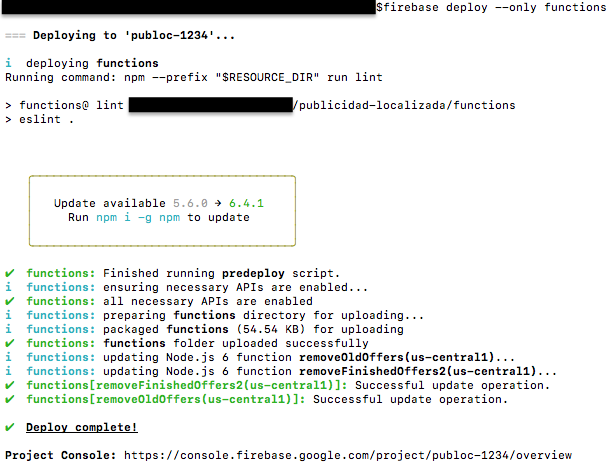
\includegraphics[scale=0.6]{figures/cloud-deploy.png}
\caption{Compilación y subida de funciones a \textit{Firebase}.\label{fig:cloud-deploy}}
\end{figure}
\end{enumerate}

\subsection{Modelo de datos}
Hay que tener en cuenta que no se trabaja con una base de datos que pueda seguir un modelo entidad relación. Por lo tanto, hay que seguir unas pautas a la hora de diseñar la estructura de los datos para un modelo de este tipo.

\subsubsection*{Evitar replicar nodos}
Para solventar el problema comentado en la sección anterior \ref{nosql}, habría que almacenar el identificador unívoco de un nodo dentro de otro para evitar replicar datos, es lo más parecido a una relación en un modelo relacional. Si hacemos esto, hay dos maneras de recuperar los datos.

\begin{enumerate}
\item\textbf{\textit{Firebase Database} + \textit{API REST}.} Lo malo es que nos vemos obligados a hacer dos peticiones o más para obtener todos los datos (depende del número de referencias a otros nodos). Esto incurre en un mayor tráfico de datos para el usuario, que lo notará en la factura, además de ralentizar las comunicaciones.

\item\textbf{\textit{Firebase Database} + \textit{Cloud Functions}.} Esta es la mejor de las soluciones, se hace una petición a una función y esta trabaja contra la base de datos, componiendo a nuestro gusta el \textit{JSON} que será devuelto.

No sólo nos ahorramos el tiempo y el coste de tener que hacer varias peticiones \textit{HTTP}, sino que también movemos al servidor la carga computacional de recolectar y juntar toda la información.
\end{enumerate}

\subsubsection*{Escalabilidad}
Es importante diseñar el modelo pensando en el futuro. Se deben estructurar los datos de manera que se pueda soportar a un gran número de usuarios. Por lo tanto, no se debe almacenar información de usuarios dentro de nodos que no son de usuarios, ver figura~\ref{fig:malaprac}. Por ejemplo, puede parecernos cómodo almacenar los identificadores de los usuarios que han escaneado una oferta dentro de la propia oferta. De esta manera, cuando un usuario pide una oferta, ya puede saber si la ha disfrutado sin necesidad de hacer otra petición para obtener sus ofertas disfrutadas.

\begin{figure}[tbp]
\centering
\subfigure{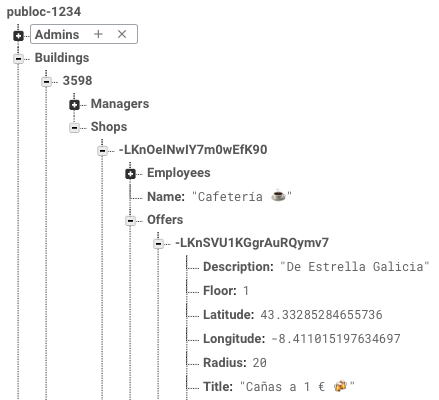
\includegraphics[width=0.65\textwidth]{figures/nodo-firebase.png}\label{fig:node}}
\vspace{3em}
\subfigure{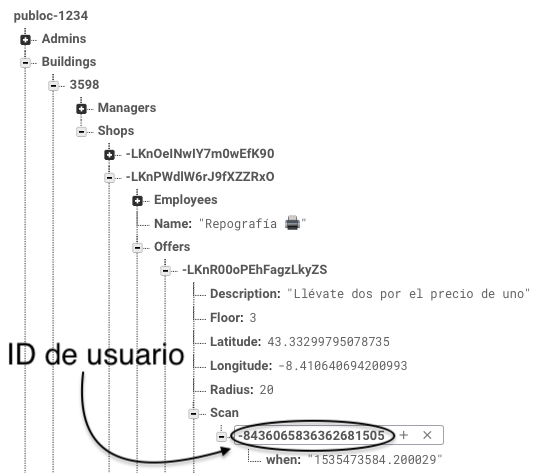
\includegraphics[width=0.65\textwidth]{figures/malaprac.png}\label{fig:malaprac}}
\caption{\textit{Firebase}: (a) Nodo de una oferta en la base de datos y (b) ejemplo de mala práctica en una estructura de datos no relacional, mezclando información de usuario con información general.}
\end{figure}

Esto funciona muy bien si la aplicación la usan cuatro personas, pero imaginemos un caso real de una aplicación con millones de usuarios que hiciera esto. En el caso de que \textit{YouTube} utilizara un modelo de datos no relacional y almacenara los \textit{likes} de usuarios en un vídeo con millones de reproducciones dentro del nodo del propio vídeo, cada vez que un usuario hiciera una petición a ese nodo, se descargaría también los datos de millones de usuarios.

Sin embargo, también se desperdician datos móviles, tiempo del usuario y memoria del dispositivo móvil. De ahí la importancia de separar los datos de usuario de los generales.

\section{Implementación de la aplicación móvil: MVC}
En esta sección se describen los procedimientos seguidos en el  desarrollo de la aplicación \textit{iOS}.
Más específicamente las capas de modelo, vista y  controlador.

\subsection{Modelo}
La implementación de la capa de modelo en una aplicación \textit{iOS} se centra en la comunicación con la base de datos: las peticiones.

%\subsubsection*{Peticiones}
Como ya se ha comentado, se emplea la librería \textit{Alamofire} para realizar las peticiones \textit{HTTP}. Una característica del lenguaje \textit{Swift}, es que permite pasar funciones como parámetros a otras funciones. De este modo se pudieron aislar los métodos que hacían las peticiones del resto del código.
Simplemente se declaran en cada controlador las funciones que se deben ejecutar al terminar cada petición y se pasan a los métodos genéricos que se comunican con la \textit{API REST}, junto con la \textit{URL}.

\begin{figure}[p]
\centering
\subfigure{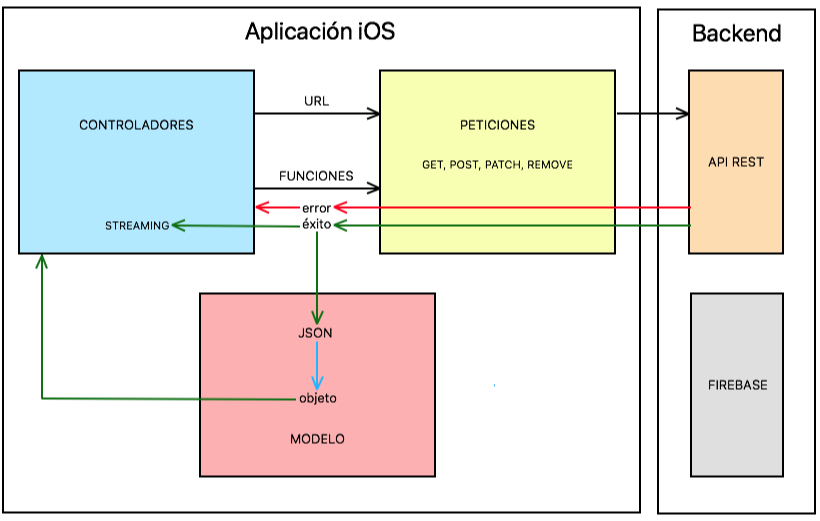
\includegraphics[width=0.89\textwidth]{figures/esquema-impl.png}\label{esquema-impl}}
\subfigure{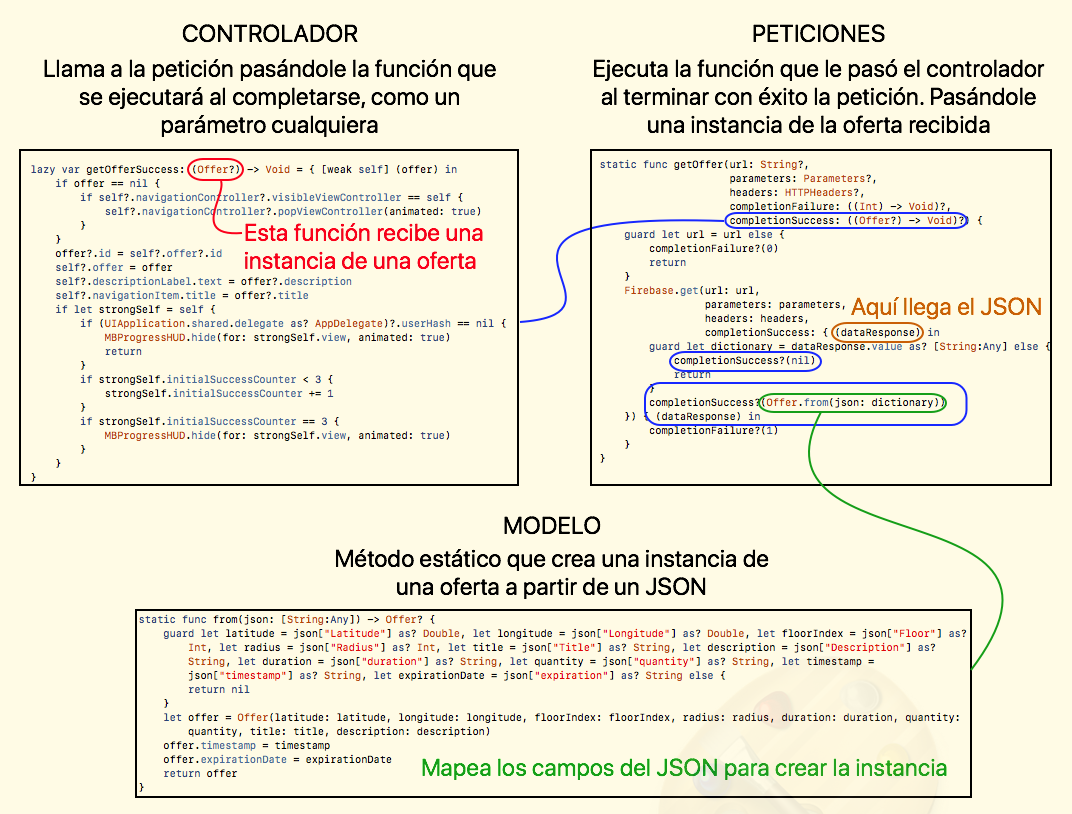
\includegraphics[width=\textwidth]{figures/ciclo.png}\label{fig:ciclo}}
\caption{MVC: (a) Comunicación de la aplicación \textit{iOS} con la \textit{API REST} y (b) funciones utilizadas en una petición.}
\end{figure}

Las peticiones se lanzan en segundo plano para no interrumpir a la aplicación.
Si se lanzasen en el \textit{thread} principal, la interfaz se quedaría bloqueada hasta que llegase la respuesta, y esto provocaría una mala experiencia de usuario. Cuando la respuesta llega, se ejecuta la función correspondiente según la respuesta obtenida, ver figura~\ref{esquema-impl}. Es recomendable mostrar un indicador de que se está cargando la información al realizar una petición, para después ocultarlo cuando la petición termina.

%\subsubsection*{Programación orientada a objetos}
Las peticiones nos devuelven una respuesta en formato \textit{JSON}, cuyos campos deben mapearse para crear instancias con las que poder trabajar. Estos métodos encargados de mapear los diccionarios \textit{JSON} funcionan como métodos constructores que devuelven una instancia que puede ser nula en caso de que no se mapeen correctamente los campos, véase la figura \ref{fig:ciclo}.

\subsection{Vista}
Antes de empezar con la implementación de la vista, se realizó un diseño con la herramienta \textit{Adobe Xd}, ver (figura~\ref{fig:adobe_xd}). Este programa es muy útil para elaborar las pantallas de la aplicación y ver como quedarían los colores, fuentes, dimensiones, etcétera; antes de ponerse a codificar. Ahorrando así mucho tiempo al programador que si no tuviese un prototipo tendría que compilar el proyecto y avanzar hasta la pantalla en cuestión para ver como quedaría cada vez que cambiase algo en la vista.

\begin{figure}[p]
\centering
\subfigure{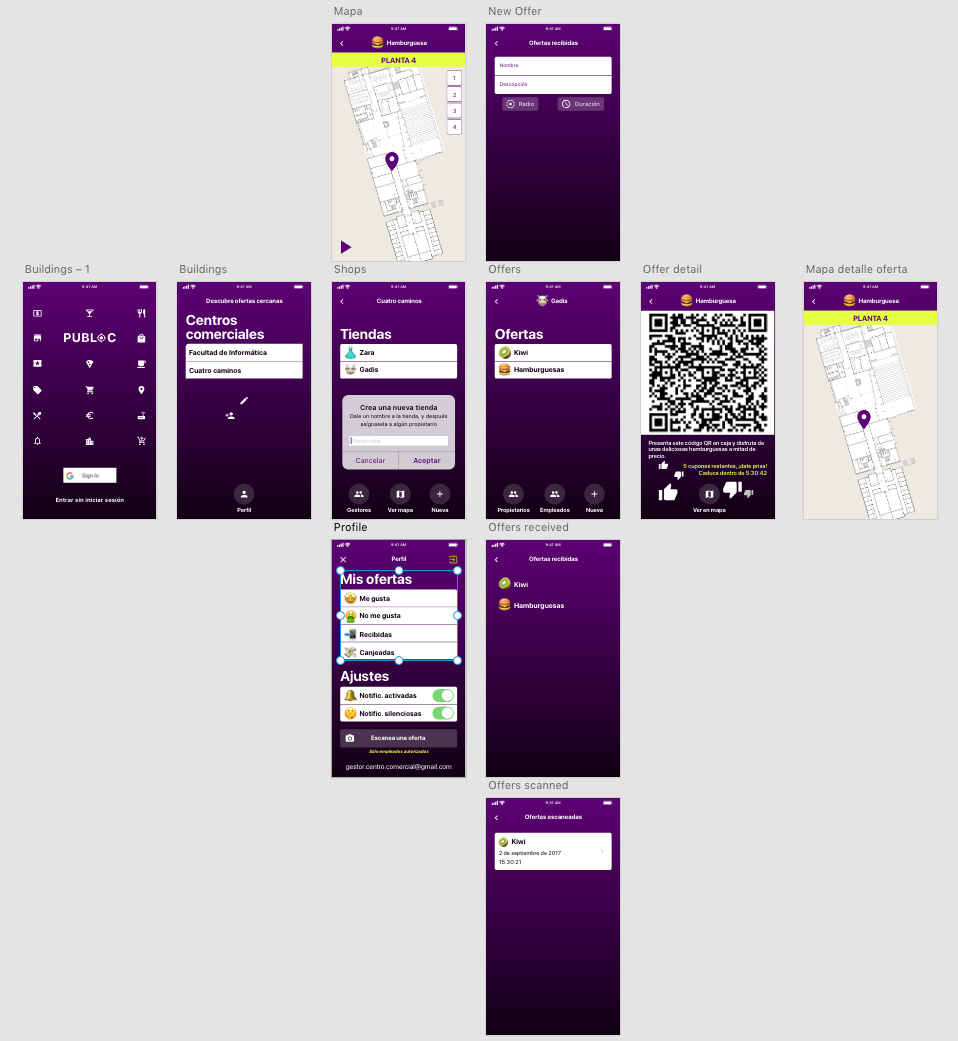
\includegraphics[width=0.85\textwidth]{figures/adobe_xd.png}\label{fig:adobe_xd}}
\subfigure{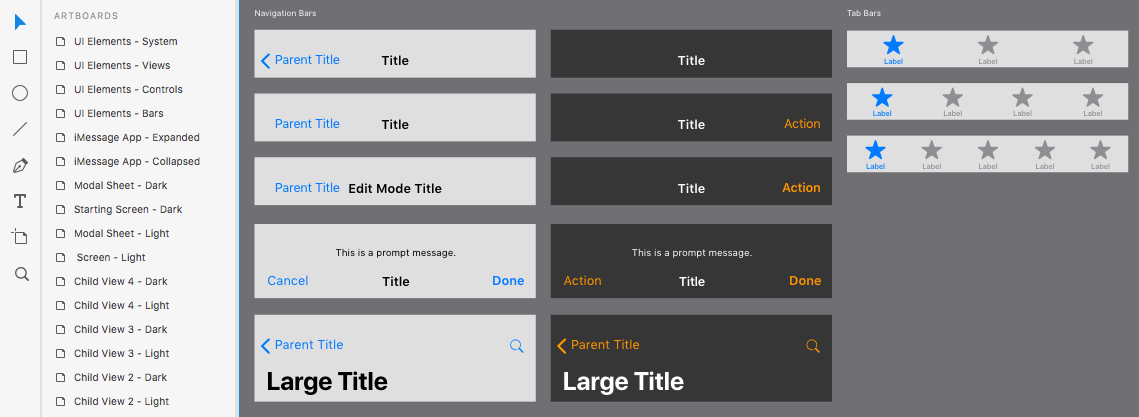
\includegraphics[width=0.89\textwidth]{figures/recursos-xd.png}\label{fig:recursos-xd}}
\caption{\textit{Adobe Xd}: (a) Captura de pantalla de la herramienta de diseño \textit{Adobe Xd} y (b) recursos oficiales de \textit{Apple}, importables para \textit{Adobe Xd}.}
\end{figure}

\textit{Adobe Xd} tiene plantillas de diversas resoluciones, que se corresponden con las resoluciones de los distintos dispositivos de \textit{Apple}, para realizar diseños sobre ellas. Además, desde la página oficial para desarrolladores de \textit{Apple} ofrecen recursos importables a \textit{Adobe Xd} \cite{noauthor_apple_nodate} como botones, cabeceras de tablas, etcétera. que cumplen con los principios de diseño recomendados para desarrollar aplicaciones \textit{iOS}, ver figura~\ref{fig:recursos-xd}.
Este programa también nos permite diseñar las transiciones entre pantallas y genera una simulación animada con la que podemos interactuar, como si de un emulador se tratase, ver figura~\ref{fig:simula-xd}.

\begin{figure}[tb]
\centering
\includegraphics[scale=0.4]{figures/simulacion-xd.png}
\caption{Transiciones entre pantallas y simulación con \textit{Adobe Xd}.\label{fig:simula-xd}}
\end{figure}

\subsubsection*{Elección y disposición de los colores}
Primero se realizó una pequeña investigación sobre el efecto que producen los colores en las personas para saber que paleta de colores queríamos utilizar. Tras leer algún artículo \cite{noauthor_color_nodate} que hablaba sobre colores que atraen más a los hombres que a las mujeres, otros que se asocian a la comida, otros a los negocios o a la naturaleza, etcétera. Se decidió utilizar como color base el morado.

Una vez elegido el color base, hay que elegir unos colores que combinen con él de manera adecuada. Para ello conviene informarse sobre el círculo cromático y qué colores se relacionan entre sí (figura~\ref{fig:relacion-colores}).
Adobe ofrece una herramienta que facilita la elección de los colores \cite{noauthor_adobe_nodate}. A partir de un color base nos da los colores que combinarían con él (figura~\ref{fig:paleta-complementaria}).

\begin{figure}[tb]
\centering
\subfigure{\includegraphics[width=0.48\linewidth]{figures/relacion-colores.png}\label{fig:relacion-colores}}
\subfigure{\includegraphics[width=0.48\linewidth]{figures/paleta-complementaria.png}\label{fig:paleta-complementaria}}
\caption{Arquitectura de colores: (a) Como combinar colores usando el círculo cromático y (b) paleta de colores utilizada, el morado y sus complementarios.}
\end{figure}


\subsubsection*{Implementación de la vista con \textit{Xcode}}
Una vez terminado el diseño, debemos incorporarlo a nuestra aplicación. Como se comentó en el capítulo \ref{planificacion_chap}, la implementación de la interfaz de usuario se dejó para el último \textit{sprint}, ya que al trabajar con una metodología \textit{SCRUM}, pueden surgir nuevas funcionalidades a medida que se avanza en el desarrollo. Esto puede tener su repercusión en la vista, siendo necesario añadir nuevos botones, tablas, mapas, etc.

\begin{figure}[tbp]
\centering
\includegraphics[scale=0.2]{figures/story-xml.png}
\caption{\textit{Interface Builder} vs \textit{xml}.\label{fig:story-xml}}
\end{figure}

El programa \textit{Xcode} permite desarrollar la vista de manera gráfica, esto facilita enormemente la tarea porque si no, habría que escribirlo todo en código \textit{xml} (figura~\ref{fig:story-xml}).
Aunque también se pueden implementar los elementos de la vista programáticamente, es decir, creándolos desde el controlador con \textit{Swift}. Este método tiene ventajas, como el hecho de tener todo en un mismo sitio bien organizado, muchas veces en el \textit{Interface Builder} se toca algo que está un poco escondido y luego pasan cosas raras en la \textit{app} y al revisar el código no se encuentra el fallo.

La principal ventaja de construir las interfaces a través del \textit{Interface Builder} es que se avanza mucho más rápido, y para desarrolladores con poca experiencia es lo más recomendable porque ves gráficamente lo que vas haciendo.

\subsection{Controlador}
En las aplicaciones \textit{iOS}, la vista y el controlador van muy unidos, de hecho uno de los componentes principales es lo que se llama \textit{UIViewController}, cual tiene varias responsabilidades que se explican a continuación.

\begin{figure}[t]
\centering
\includegraphics[scale=0.4]{figures/outlets.jpg}
\caption{Para referenciar un elemento de la vista basta con arrastrarlo desde \textit{Interface Builder}.\label{fig:outlets}}
\end{figure}


\paragraph{Actualizar los contenidos de las vistas.} Normalmente suele ocurrir en respuesta a cambios en los datos subyacentes. Podemos vincular un \textit{UIViewController} con un \textit{UIStoryBoard} que es como se conoce al \textit{Interface Builder}. Los elementos de la interfaz se pueden referenciar desde el controlador para modificarlos programáticamente, y se llaman \textit{Outlets}, ver figura~\ref{fig:outlets}.

\begin{figure}[tb]
\centering
\includegraphics[scale=0.2]{figures/segues.png}
\caption{En \textit{Interface Builder} se definen las relaciones entre controladores (\textit{Segues}). \label{fig:segues}}
\end{figure}

\paragraph{Responder ante las interacciones del usuario con las vistas.} Del mismo modo que vimos en la figura \ref{fig:outlets}, podemos referenciar no sólo los elementos de la interfaz desde el controlador, sino también las distintas acciones que pueden realizar en respuesta a acciones del usuario, y se llaman \textit{Actions}.

\paragraph{Coordinarse con los otros objetos.} Incluyendo otros \textit{UIViewControllers}. Como vimos en el anterior capítulo, se navega de un controlador a otro a mediante el controlador padre o también pueden presentarse los controladores entre ellos. Estas relaciones pueden definirse también en el \textit{Interface Builder}, y se llaman \textit{Segues}, ver figura~\ref{fig:segues}.


























\chapter{Pruebas}
En esta sección explicaremos las pruebas realizadas al final de cada \textit{sprint}, así como las herramientas utilizadas y un cuestionario de calidad.

% Pruebas de final de sprint
\section{Pruebas de final de \textit{sprint}}
Al final de cada \textit{sprint} se han realizado las pruebas necesarias para verificar que las funcionalidades introducidas en el mismo, funcionan correctamente. Además, se suele dar un repaso a las funcionalidades anteriores para ver que se integran correctamente con las nuevas, surgiendo a veces nuevas ideas o soluciones que se introducen en el ciclo de desarrollo \textit{SCRUM}.

\paragraph{\textit{Sprint} 1.} Se comprobó cuidadosamente que los planos obtenidos de \textit{Situm} se solapasen correctamente sobre el mapa de \textit{Google Maps}, sin pisarse los unos a los otros.

\paragraph{\textit{Sprint} 2.} Se realizó un primer diseño de la estructura de base de datos, evitando las malas prácticas en las que se suele incurrir al diseñar un modelo no relacional. Aún a sabiendas de que esa estructura podría modificarse en un futuro, en caso de que apareciesen nuevas funcionalidades o se detectasen fallos.

\paragraph{\textit{Sprint} 3.} Se probaron las operaciones \textit{CRUD} (\textit{create}, \textit{read}, \textit{update}, \textit{delete}) con ofertas y tiendas. Pero antes de nada, hubo que verificar que todas las peticiones funcionaban correctamente y que no alteraban la estructura de datos deseada en \textit{Firebase}, antes de incorporarlas a la aplicación.

\paragraph{\textit{Sprint} 4.} Para comprobar que las notificaciones saltaban correctamente cuando un usuario entraba en el campo de acción de una oferta, hubo que generar un fichero \textit{JSON} con múltiples coordenadas, cada una de las cuales representaba un punto en una ruta a través de la Facultad de Informática de A Coruña (edificio utilizado para las pruebas).

\paragraph{\textit{Sprint} 5.}Las pruebas consistieron en comprobar que ningún usuario podía acceder a funcionalidades que no eran propias de su rol.

\paragraph{\textit{Sprint} 6.}Se puso especial atención al funcionamiento de las \textit{Cloud Functions} y los atajos de \textit{Siri}, puesto que ambas tecnologías se encuentran en estado de beta. Respecto al diseño de la interfaz, se realizaron pruebas en distintos tamaños de pantalla para ver como quedaría en los demás dispositivos de la marca, no sólo en el \textit{iPhone SE}.

% Pruebas de caja negra
\section{Pruebas de caja negra}
A continuación se hablará sobre los módulos de la \textit{app} que pasaron por estas pruebas.

\paragraph{Aplicación \textit{iOS}.}Para probar ciertos aspectos de la aplicación, se simulaban los datos antes de implementar la obtención de los mismos. Un ejemplo claro de esto es la simulación de la ubicación, utilizada para ver si las notificaciones se lanzaban correctamente.

\paragraph{\textit{Firebase}.}Para probar como se estructuraban los datos en la base de datos, para verificar que los identificadores de los nodos se generaban de manera adecuada, o que no se permitía hacer peticiones a usuarios que no estaban autenticados, etcétera.

Se utilizaron herramientas externas como \textit{Postman} para probar las peticiones antes de añadirlas de manera definitiva a la aplicación. También \textit{Firebase} permite añadir a mano nodos desde la consola, así podíamos probar que las \textit{Cloud Functions} hacían lo que se esperaba de ellas.

% Cuestionarios de calidad
\section{Cuestionarios de calidad}
Se realizó un estudio con 10 usuarios de diferentes edades y gustos, la mayoría de ellos no estaban familiarizados con el desarrollo \textit{software}, pero todos encajaban en el perfil de posibles usuarios de una aplicación de este tipo, ver la tabla~\ref{tab:encuesta}.

En la encuesta se valoraron las siguientes facetas de la aplicación:

\begin{itemize}
\item{}\textbf{Usabilidad.} Facilidad de uso que ofrece la aplicación para los nuevos usuarios que no la conocen.
\item{}\textbf{Interfaz.} Impresión que ofrece a simple vista.
\item{}\textbf{Funcionalidad.} Utilidad de la aplicación, comparándola con otras ya existentes en el mercado.
\item{}\textbf{Rendimiento.} Fluidez, retardos al cargar los datos. Repercusión sobre los recursos del teléfono: batería, memoria, etcétera.
\end{itemize}

\begin{table}[tbp]
\begin{center}
\small
\begin{tabular}{|l|c|}
\hline 
Preguntas & Valoración  \\
\hline 
\hline
\textbf{Usabilidad} & \textbf{6/7} \\
\hline
¿Es intuitiva? & 6/7 \\
\hline
¿Es fácil de usar? & 7/7 \\
\hline
¿Es pequeña la curva de aprendizaje? & 5/7 \\
\hline
\textbf{Interfaz} & \textbf{6/7} \\ 
\hline
¿Tiene un diseño atractivo? & 6/7 \\
\hline
¿Es fácil moverse por la aplicación? & 6/7 \\
\hline
¿Se comprende en todo momento lo que hay en pantalla? & 6/7 \\
\hline
\textbf{Funcionalidad} & \textbf{7/7} \\ 
\hline
¿Te resulta útil? & 7/7 \\
\hline
¿La recomendarías a otras personas? & 7/7 \\
\hline
¿Ofrece funcionalidades que no habías visto nunca en una \textit{app}? & 7/7 \\
\hline
\textbf{Rendimiento} & \textbf{6/7} \\ 
\hline
¿Es fluida? & 6/7 \\
\hline
¿Tarda mucho en arrancar? & 5/7 \\
\hline
¿Afecta al rendimiento de tu teléfono móvil? & 7/7 \\
\hline
\end{tabular}
\caption{Resultados de la encuesta.\label{tab:encuesta}}
\end{center}
\end{table}

Como conclusión, en lo que destaca principalmente la \textit{app}, es en su utilidad. No existen muchas aplicaciones que ofrezcan este tipo de funcionalidades, y las personas que suelen ir de compras a menudo, la encuentran muy atractiva.

Por otro lado, es lógico que no haya aplicaciones de este tipo, debido a la dificultad de su implantación.

\chapter{Conclusiones y trabajo futuro}
En este capítulo se realizará una valoración final sobre lo que se hizo a lo largo de todo el proyecto, se hablará también de las lecciones aprendidas durante el desarrollo del mismo y finalmente, sobre el rumbo que podría tomar en el futuro.

%% Conclusiones
\section{Conclusiones}

El resultado obtenido fue mejor de lo que se esperaba. Todos los requisitos se cumplieron con éxito e incluso se añadió alguno nuevo.

En este trabajo se ha creado una plataforma para crear y gestionar publicidad geolocalizada. 
El objetivo ha sido utilizar los teléfonos móviles como
canal de comunicacion entre comercios y clientes.
Por un lado, se emplea la información sobre la  posición de un usuario para lanzar notificaciones sobre ofertas y descuentos disponibles a su alrededor.
Por otro lado, una vez dados de alta en el sistema, los propietarios de las tiendas pueden crear, gestionar y publicar sus propias ofertas y descuentos.

\paragraph{Sistema modular y distribuido.} Se ha diseñado una arquitectura centralizada alrededor de un servicio de \emph{Backend} basado en una base de datos \emph{Firebase}, un sistema de localización basado en \emph{Situm} y una aplicación móvil \emph{iOS} que facilita el acceso a todo el sistema.
De esta manera, sería relativamente simple sustituir algún componente o integrar nuevos servicios sin realizar grandes cambios en el sistema. También sería relativamente sencillo añadir una aplicación para el sistema operativo \emph{Android}.

\paragraph{Intercambios en tiempo real.} El sistema ha sido diseñado alrededor de \emph{Firebase} con el objetivo de que las comunicaciones sean prácticamente intantáneas. Es decir, los cambios de los datos (posición, ofertas, canjeos, perfiles, etc.), se actualizan de forma prácticamente simultánea tanto en el servidor como en los teléfonos móviles.

\paragraph{Sistema de roles.} Para facilitar la interacción entre los diferentes actores del sistema y evitar injerencias, se ha creado una jerarquía de roles para todos los usuarios.
Los roles definidos son: administrador de la plataforma, gestor del centro comercial, propietario de una tienda, empleado de una tienda, cliente autenticado y cliente sin autenticar. 
Cada rol tiene asociado acciones específicas, no accesibles al resto.
De todos modos, en modo depuración se han desbloqueado todas las funcionalidades en algunas cuentas para tener un acceso sencillo a todas las acciones posible y facilitar las pruebas.

\paragraph{Aplicación \emph{iOS}.} Es el componente encargado de acceder y gestionar toda la información de la plataforma.
Dispone de una interfaz  sencilla y muy intuitiva para que el usuario no se sienta abrumado. Además, trata de seguir todas las líneas de diseño marcadas para el sistema \textit{iOS}.
Cada usuario, en función de su rol, tendrá acceso a todas las acciones que puede realizar en la plataforma.

\paragraph{Gestión de ofertas y tiendas.} Los datos generales de la aplicación se almacenan en \textit{Firebase}, especialmente toda la información sobre tiendas y ofertas. 
Cualquier usuario podrá ver las tiendas y todas sus ofertas, pero sólo si está autenticado podrá indicar si le gusta o no.
También cada usuario puede comprobar en su perfil que ofertas le gusta, cuales no, las que ha canjeado y aquellas con las que se ha cruzado.
Sólo los gestores de centro comercial pueden añadir, modificar o eliminar una tienda dentro de la aplicación \emph{iOS}.
Para gestionar las ofertas tiene que ser el propietario de la tienda. 
Cualquier empleado de la tienda, puede canjear una oferta.

\paragraph{Notificaciones.} Cada oferta tiene asociado un radio de acción y cuando un usuario está cerca, salta una notificación en su teléfono móvil, aunque la aplicación no esté en primer plano. 
A partir de la notificación se podrá ver los detalles de la oferta.
También se puede obtener un código \textit{QR} para canjear la oferta en la tienda. 
Si el usuario no quiere ser molestado, podrá desactivar o silenciar las notificaciones de su móvil, pero sin miedo a perderse ninguna oferta, porque siempre que quiera podrá revisar las ofertas que le han llegado.

\paragraph{Canjeo de ofertas.} Las ofertas se canjean por medio de códigos \emph{QR} creados (rol de usuario) y leídos (rol empleado) por la propia aplicación. La aplicación también deja constancia de qué usuarios han disfruta (canjeado) cada oferta.
Como ya se ha comentado, en el perfil de cada usuario también se puede añadir qué ofertas le gustan o no.

\paragraph{Ofertas con caducidad.} Se han diseñado ofertas que puedan tener una fecha de caducidad o un número de unidades limitadas. 
También se han diseñado mecanismos para mantener la coherencia de la información (por ejemplo, si hay varios empleados canjeando ofertas). Las ofertas se canjean estrictamente en el orden de llegada.
El objetivo de ambas funcionalidades ha sido incentivar el consumo, dado que al limitar el tiempo o el número de unidades disponible, se intenta crear la sensación de que debe aprovechar la oportunidad.

\paragraph{Escaneo de ofertas con \textit{Siri}.} 
Se ha implementado un atajo de \emph{Siri} para lanzar el escáner de códigos \emph{QR} mediante un comando de voz.
De esta forma, el uso de la aplicación es más intuitiva y cómoda.
Esta funcionalidad ha sido posible porque durante el desarrollo del proyecto \textit{Apple} ha lanzado la beta de \textit{iOS} 12, que permite asociar acciones de una aplicación con comandos de voz personalizados para ejecutarlos desde \textit{Siri}. 

\paragraph{Sistema de localización del usuario.} Se ha integrado el servicio de localización de \textit{Situm}, que nos permite conocer la posición de un teléfono móvil tanto en exteriores (usando el GPS) como en interiores (una vez calibrado el edificio en cuestión).
Sin embargo, debido a una conocida limitación de \textit{iOS} para acceder a cierta información sobre las señales \textit{WiFi}, la localización sólo es funcional si el entorno dispone de balizas \emph{Bluetooth}.
Para simplificar la realización del proyecto, se decidió implementar un mecanismo para simular posiciones en el interior de edificios. 

\paragraph{Pruebas finales exitosas.} Se han realizado diferentes pruebas en la Facultad de Informática de la Universidade da Coruña, incluyendo cambios de planta, que han demostrado la viabilidad de la propuesta realizada.
También se ha realizado una encuesta a varios usuarios que han probado la aplicación \emph{iOS} en diferentes condiciones y con diferentes roles. Los resultados obtenidos son muy prometedores.



%% Lecciones aprendidas
\section{Lecciones aprendidas}
A continuación, algunas de las lecciones aprendidas tras la realización de este proyecto.

\paragraph{Dejar el diseño de la interfaz para el final.}
Nunca se sabe que funcionalidades o limitaciones van a surgir a lo largo de todo el desarrollo, así que el apartado de diseño debe ser de lo último de lo que nos preocupemos.

\paragraph{Ser organizados desde el principio.}
Con las prisas se pierden buenos hábitos de programación: no se organizan los ficheros correctamente, se replica código, etcétera. Puede que ser ordenados nos consuma algo más de tiempo, pero a la larga se agradece.

\paragraph{Ir tomando nota siempre.}
Todos aquellos fallos o ideas que vayan surgiendo a lo largo del desarrollo deben anotarse. A veces pensamos que nos vamos a acordar seguro, pero rápidamente surgen otros problemas que nos hacen olvidarnos de los anteriores.

\paragraph{Hacer \textit{commits} con frecuencia.}
Al trabajar con más gente es normal que se hagan muchos \textit{commits} para ir dejando constancia al resto del equipo de lo que se va haciendo. Pero cuando se trabaja solo, se tiende a ser menos organizado con el control de versiones: \textit{commiteando} con menos frecuencia de la debida, no poniendo nombres adecuados a los \textit{commits}, etcétera.
Esto provoca que muchas veces perdamos cambios importantes y dificulta la detección de fallos. Porque si hay muchas diferencias entre un \textit{commit} y su predecesor, nos costará más identificar un fallo concreto.

\paragraph{El código en \textit{Backend} es esencial.}
Trabajar contra un servidor que sólo nos permite almacenar la información es inviable, ya que con el tiempo surge la necesidad de ejecutar código porque van apareciendo  funcionalidades más complejas. Aunque existen servicios de \textit{Backend} externos, la opción que aporta una mayor flexibilidad siempre es utilizar nuestros propios servidores siempre que tengamos esa posibilidad.

\paragraph{Documentarse bien antes de trabajar.}
Es importante estudiar todas las maneras existentes de hacer algo antes de hacerlo. Sobre todo a la hora de externalizar una funcionalidad, debemos comparar las tarifas y funcionalidades que ofrece cada plataforma y escoger la que más se adapte a nuestras necesidades. Nunca hay que lanzarse de cabeza a una solución, sin explorar todas las alternativas.

\paragraph{Intentar prescindir de librerías externas.}
Lo más rápido a la hora de integrar una funcionalidad en la aplicación, es buscar una librería de terceros. Pero debemos evitar esto porque no conocemos la calidad ni la fiabilidad del código que estamos introduciendo en nuestro proyecto. Siempre debemos implementar nosotros mismos todo lo que podamos; aunque ralentice el desarrollo, con el tiempo lo agradeceremos, cogeremos más experiencia como desarrolladores y no usaremos código desconocido.

Finalmente, acabaremos desarrollando nuestras propias librerías con las soluciones ingeniosas que le hayamos dado a los problemas que han ido apareciendo y podremos utilizarlas en todos nuestros proyectos futuros.

\paragraph{Gestionar bien la memoria desde el principio.}
No se debe esperar a que aparezcan los primeros \textit{crashes} por tener una mala gestión de la memoria. Debemos ir haciendo escaneos periódicos a la aplicación en busca de recursos que no se liberan correctamente, referencias circulares y fugas de memoria  \cite{leandro_perez_memory_nodate}.

\paragraph{Pensar en la privacidad del cliente.}
Con el planteamiento actual, se obliga al cliente a suministrar los planos y calibraciones de sus edificios al administrador de la plataforma para que los suba al \textit{Situm Dashboard}. Pueden perderse clientes potenciales por esto, ya que quizás no les guste tener que mediar siempre con el administrador de la plataforma.

\paragraph{Tener en cuenta la legislación.}
Antes de lanzar una aplicación al mercado, debe hacerse un estudio de las leyes de aquellos países en los que va a estar disponible. Porque si no, corremos el riesgo de inclumpir alguna ley o normativa y vernos metidos en un lío.

Por ejemplo, hace poco se entró en vigor el Reglamento General de Protección de Datos, una de las diferencias con su predecesor es que no da por válido el consentimiento tácito para la recolección de datos del usuario. Todas las aplicaciones que pidan información personal al usuario, deben tenerlo en cuenta.

% Trabajo futuro
\section{Trabajo futuro}
En esta sección, se hablará sobre algunas de las posibles mejoras a añadir en \textit{sprints} futuros.

\paragraph{Rediseño del modelo con \textit{Cloud Functions}.}
Cuando se empezó el proyecto, no se tenía en mente utilizar esta funcionalidad de \textit{Firebase}. Pero tras la incorporación al ciclo de desarrollo de una funcionalidad que necesitaba de la ejecución de código en servidor, se vio el potencial de esta herramienta.

Muchas tareas que fueron implementadas únicamente con peticiones a la \textit{API REST} e incluso la propia estructura de la base de datos, podrían simplificarse gracias a esto, haciendo una aplicación más rápida y eficiente.

\paragraph{Añadir un servicio de analítica.}
Cuando una aplicación empieza a tener un volumen de usuarios considerable, debe incorporar herramientas de este tipo. Cuando hay un \textit{crash} en una aplicación y el sistema operativo la cierra, se produce una impresión muy negativa en el usuario. Por ello, es importante tener una herramienta que monitoree la aplicación y que proporcione información de los \textit{crashes} a los desarrolladores.

También es interesante conocer como crece la aplicación, el número de nuevos usuarios diarios, el tiempo que pasa la gente de media en nuestra aplicación, etcétera. Todas estas estadísticas ayudan a comprender como actúa el cliente, y por lo tanto muy importante para mejorar.

\paragraph{Probar otras plataformas de posicionamiento en interiores.}
Gracias a que hemos diseñado la aplicación de forma modular, ahora somos libres de cambiar de servicio proveedor de localización, actualmente se utiliza \textit{Situm}, pero hay otros. Un posible \textit{sprint}, podría ser hacer un estudio de mercado y probar otras plataformas de localización en interiores para ver si encontramos alguna que nos guste más.

%% Subir la aplicación a la App Store
\subsection{Subir la aplicación a la \textit{App Store}}
Finalmente, una vez se tenga un producto estable sin simulaciones, podría subirse una versión a la \textit{App Store}. Pero quedaría muy mal hacerlo sin centros comerciales, así que antes habría que buscar clientes interesados que nos diesen autorización para subir a nuestra plataforma sus planos y calibraciones.

Habría que llevar a cabo un proceso de promoción previo al lanzamiento de la aplicación, contactar con varios centros comerciales, eventos, comerciantes, etcétera; para establecer un modelo de negocio. Calibrar los entornos, realizar pruebas reales, dar unas cuantas tiendas de alta, crear ofertas y establecer roles, preparar una buena inauguración. Todo esto es esencial para lanzar una aplicación de este tipo al mercado y que triunfe. Si se lanza vacía, la gente la va a descargar y según la abran y no vean nada, la borrarán de sus teléfonos y se quedarán con una impresión negativa de la \textit{app} para siempre.

Este proyecto es demasiado ambicioso para una sola persona, lanzar y mantener una aplicación de este tipo necesitaría muchas horas de trabajo de todo un equipo. Por ello, este proyecto nunca tuvo como objetivo la creación de una aplicación real y comercializable. La finalidad siempre fue la de desarrollar un prototipo de lo que en un futuro podría llegar a ser una de las muchas utilidades de la incipiente tecnología de posicionamiento en interiores.


% Apéndices
\appendix

\chapter{Instalación y uso de la \emph{app}}
Aquí se explican los primeros pasos y consideraciones a seguir para que todo aquel que esté interesado en utilizar la \textit{app}.
\section{Requisitos}
Esta aplicación sólo puede instalarse en dispositivos que tengan \textit{iOS 11.3} o posterior, ver figura~\ref{fig:target}. Además, los atajos de \textit{Siri} sólo funcionan a partir de \textit{iOS 12}, por lo tanto esta funcionalidad no estaría disponible para dispositivos que no estuviesen actualizados. Todos los dispositivos que soportan \textit{iOS 11}, también soportan \textit{iOS 12}.

\begin{figure}[tbp]
\centering
\includegraphics[scale=0.6]{figures/target.png}
\caption{Requisitos mínimos del sistema operativo.\label{fig:target}}
\end{figure}

\section{Instalación}
Todo aquel que quiera empezar a utilizar la aplicación sólo tiene que instalarla en su teléfono  \textit{iOS}. No está disponible en la \textit{Apple Store} todavía, así que tendría que obtener el ejecutable por otras fuentes e instalarlo manualmente \cite{noauthor_como_nodate}.

\section{Manual de usuario\label{apen:manual-usuario}}
En esta sección, se guiará al usuario a través de las diferentes pantallas de la aplicación, explicándole el contenido de las mismas y como debe interactuar con ellas.

\subsection{Pantallas principales}
Aquí hablaremos sobre las pantallas fundamentales de la aplicación, desde el inicio de sesión hasta el listado de ofertas.

\paragraph{Pantalla de inicio.} Se presenta la aplicación y se da la opción al usuario de iniciar sesión con \textit{Google} o de entrar directamente, ver figura~\ref{fig:inicio}.

\begin{figure}[tbp]
\centering
\includegraphics[scale=0.4]{figures/inicio.png}
\caption{Proceso de inicio y autenticación con \textit{Google}.\label{fig:inicio}}
\end{figure}

\paragraph{Centros comerciales.} La siguiente pantalla que se presenta es la misma independientemente de si el usuario está autenticado o no. Contiene una tabla en la que aparecen todos los centros comerciales que están dados de alta en \textit{Situm Dashboard}, en la parte inferior de la pantalla encontraremos un botón que permite al usuario ver su perfil y realizar algunos ajustes, ver subfigura~\ref{ref:centros-comerciales}.

\begin{figure}[tbp]
\centering
\subfigure{\includegraphics[scale=0.2]{figures/centros-comerciales.jpeg}\label{ref:centros-comerciales}}
\subfigure{\includegraphics[scale=0.4]{figures/tiendas-map.jpeg}\label{ref:tiendas-map}}
\subfigure{\includegraphics[scale=0.4]{figures/ofertas.jpeg}\label{ref:ofertas}}
\caption{Tablas: (a) Centros comerciales, (b) tiendas de un centro comercial y (c) ofertas de una tienda.}
\end{figure}

\paragraph{Tiendas.} Si el usuario selecciona un centro comercial entonces se mostrarán las tiendas que están dadas de alta en la plataforma. En esta pantalla también hay un botón que nos llevará a un mapa en el cual hemos cargado los planos del edificio, ver subfigura~\ref{ref:tiendas-map}.

\paragraph{Ofertas.} Y si finalmente el usuario selecciona una tienda, podrá ver las ofertas que ha dado de alta el propietario de la misma, ver subfigura~\ref{ref:ofertas}. Seleccionando una, se verá el detalle de la misma.

\subsection{Detalle de oferta}
Cuando seleccionamos una oferta concreta, se mostrará una pantalla con más información, ver subfigura~\ref{fig:detail}. Esta pantalla se merece una subsección para ella sola porque tiene muchos componentes.

\paragraph{Código \textit{QR}.} El cliente deberá mostrarlo al empleado de tienda para canjear la oferta, sólo aparecerá en caso de que el usuario esté autenticado. Si no, se mostrará un botón para que inicie sesión con \textit{Google} si así lo desea.

\paragraph{Descripción.} Breve texto descriptivo sobre la oferta.

\paragraph{Contador de ofertas restantes.} Aquí se mostrarán en tiempo real las ofertas que quedan disponibles.

\paragraph{Cuenta atrás.} Indica el tiempo que queda para que caduque la oferta.

\paragraph{Botones de \textit{like}/\textit{dislike}.} Así el usuario podrá indicar si no le interesa que se le notifique esa oferta dándole a \textit{like}. Pero si seleccionase \textit{dislike}, entonces la oferta quedaría archivada en el listado de ofertas favoritas que comentaremos más adelante. Al igual que el código \textit{QR}, estas funciones sólo estarán activadas en caso de que el usuario este autenticado, en caso contrario, los botones aparecerán, pero deshabilitados.

\paragraph{Ver en mapa.} Mostrará la situación de la oferta en el plano del edificio, ver subfigura~\ref{fig:map-detail}.

\begin{figure}[tbp]
\centering
\subfigure{\includegraphics[scale=0.4]{figures/detail.png}\label{fig:detail}}
\subfigure{\includegraphics[scale=0.2]{figures/map-detail.jpeg}\label{fig:map-detail}}
\caption{Detalle oferta: (a) Oferta en detalle para un usuario sin autenticar/autenticado y (b) mapa que muestra únicamente una oferta.}
\end{figure}

\subsection{Mapas}
Aquí hablaremos sobre las pantallas que contienen mapas, en la aplicación nos encontramos con varias, que a pesar de ser parecidas, tienen propósitos diferentes.

\paragraph{Mapa completo del edificio.} Aquí el usuario puede explorar el edificio, seleccionando la planta que le interesa. También podrá ver la situación de todas las ofertas que no haya rechazado previamente y acceder al detalle de las mismas seleccionando el marcador en el mapa. Si se encuentra en el centro comercial, podrá ver también su posición con exactitud, ver subfigura~\ref{fig:building-map}.

\begin{figure}[tbp]
\centering
\subfigure{\includegraphics[scale=0.2]{figures/building-map.jpeg}\label{fig:building-map}}
\subfigure{\includegraphics[scale=0.2]{figures/map-newoffer.png}\label{fig:newoffer}}
\caption{Mapas: (a) Mapa completo del edificio (aparece el icono de pausa porque es una simulación) y (b) marcar en el mapa la posición de la nueva oferta.}
\end{figure}

\paragraph{Situación de una oferta concreta en el mapa.} A partir del detalle de una oferta podemos ver su posición en el mapa. Se indicará la planta en la que se encuentra y no se podrá seleccionar otra, ver subfigura~\ref{fig:map-detail}.

\paragraph{Creación de una nueva oferta.} Cuando un usuario con rol de \textit{Propietario de tienda} quiere crear una nueva oferta, tiene que seleccionar la ubicación de la misma en el plano del centro comercial, ver subfigura~\ref{fig:newoffer}.

\subsection{Pantalla de perfil}
Si el usuario está autenticado, podrá ver las ofertas recibidas, las favoritas, las que no le interesan y las que ha canjeado. Estas funciones están deshabilitadas para usuarios que no han iniciado sesió. Además de las ofertas del usuario, en la pantalla de perfil se mostrarán ajustes relativos a las notificaciones, los cuales están disponibles para cualquier tipo de usuario, ver subfigura~\ref{fig:notif}. También encontraremos en esta pantalla, un botón que abrirá el escáner de códigos QR, para que los empleados puedan cajear ofertas, ver subfigura~\ref{fig:no-auth-qr}.

\begin{figure}[tbp]
\centering
\subfigure{\includegraphics[scale=0.2]{figures/perfil.png}\label{fig:notif}}
\subfigure{\includegraphics[scale=0.2]{figures/no-auth-qr.PNG}\label{fig:no-auth-qr}}
\caption{Perfil: (a) Usuario no autenticado vs usuario autenticado y (b) escáner con alerta informando al empleado de que no está autorizado para canjear esa oferta.}
\end{figure}

\paragraph{Ofertas favoritas o \textit{likes}.} Son aquellas ofertas en las que hemos pulsado el botón de \textit{like}. El usuario siempre tiene la opción de eliminar una oferta de favoritas o de indicar que ya no le gusta, ver figura~\ref{fig:megustan}.

\begin{figure}[tbp]
\centering
\includegraphics[scale=0.2]{figures/megustan.png}
\caption{Ofertas favoritas del usuario, deslizando la celda aparecen las opciones de borrar o de mover a rechazadas.\label{fig:megustan}}
\end{figure}

\paragraph{Ofertas rechazadas o \textit{dislikes}.} Son aquellas ofertas en las que hemos pulsado el botón de \textit{dislike}. El usuario siempre tiene la opción de eliminar una oferta de rechazadas o de indicar que ha cambiado de opinión y que ha decidido que le gusta. La pantalla sería exactamente igual que la de los \textit{likes} (figura~\ref{fig:megustan}), simplemente se cambiaría el botón de \textit{dislike} por el de \textit{like}.

\paragraph{Ofertas recibidas.\label{item:recibidas}} Estas son las ofertas con las que se ha cruzado el usuario. Se lleva un registro de las mismas, por si acaso no tenía activadas las notificaciones o no estaba atento a la aplicación cuando se las cruzó. De esta manera, puede llegar a casa y revisarlas para indicar cuales le gustan y cuales no, o simplemente ignorarlas. Cuando un usuario indica que una de estas ofertas le gusta o no, desaparece del listado de ofertas recibidas y pasa a favoritas o rechazadas, ver figura~\ref{fig:recibidas}.

\begin{figure}[tbp]
\centering
\includegraphics[scale=0.2]{figures/recibidas.png}
\caption{Ofertas recibidas, deslizando la celda aparecen las opciones de borrar o de \textit{like}/\textit{dislike}.\label{fig:recibidas}}
\end{figure}

\paragraph{Ofertas canjeadas.} Estas son las ofertas que el usuario ha canjeado. Se lleva un registro de las mismas por motivos de seguridad, en caso de que el usuario quiera reclamar algo se podrá ver con facilidad si ya ha disfrutado la oferta o no. Esta pantalla es exactamente igual que las anteriormente comentadas (figura~\ref{fig:recibidas} y figura~\ref{fig:megustan}), con la diferencia de que al deslizar la celda no encontramos ningún botón ni de me gusta/no me gusta, ni de eliminar. Ya que no se quiere que las ofertas desaparezcan de ahí.

\subsection{Roles}
Hasta ahora hemos visto la aplicación como la vería un usuario normal, autenticado o sin autenticar, salvo por la subfigura~\ref{fig:newoffer} que corresponde a una pantalla que sólo los propietarios de las tiendas podrán ver. A continuación, veremos como se han distribuido las acciones propias de los otros cuatro roles.

\paragraph{Administrador de la plataforma.} Cuando el administrador de la plataforma selecciona un centro comercial, se le ofrece la posibilidad de añadir un nuevo gestor. La pantalla de añadir un nuevo rol es igual para gestores, propietarios y empleados \ref{addrol}.

\paragraph{Gestor de un centro comercial.} Cuando un usuario es nombrado gestor de un centro comercial, en su pantalla aparece en tiempo real un botón que le permite añadir una nueva tienda, llevándolo a otra muy similar a la de añadir rol en la que simplemente le pregunta el nombre del establecimiento. Y si está en la pantalla correspondiente a una tienda, aparecerá un botón que le permitirá añadir un propietario a la misma, ver figura~\ref{addrol}.

\begin{figure}[tbp]
\centering
\includegraphics[scale=0.2]{figures/anadir-rol.png}
\caption{Estas capturas fueron tomadas con la aplicación en modo desarrollo con todas las funcionalidades desbloqueadas, por eso aparecen los botones de \textit{Empleados} y \textit{Propietarios}, dos acciones que corresponden a roles diferentes y que no deberían aparecer en la misma pantalla.\label{addrol}}
\end{figure}

\paragraph{Propietario de una tienda.} Cuando un usuario es nombrado propietario de una tienda, aparecerá en su pantalla la posibilidad de añadir un empleado o una oferta a la misma. Para añadir una oferta, primero hay que marcar su posición en el plano, como en la subfigura~\ref{fig:newoffer} y a continuación, darle un nombre, una descripción, el radio de acción, la duración y el número de unidades disponibles, ver figura~\ref{fig:newoffer2}.

\begin{figure}[tbp]
\centering
\includegraphics[scale=0.2]{figures/newoffer2.png}
\caption{Cuando el propietario selecciona alguno de los botones de radio de acción, duración o unidades; se muestra un selector.\label{fig:newoffer2}}
\end{figure}

\paragraph{Empleado de una tienda.} Cuando un usuario es nombrado empleado de una tienda, podrá empezar a canjear ofertas de la misma. Se hablará más a fondo sobre esto, más adelante \ref{qr}.


\subsection{Notificaciones}
Cuando un cliente va caminando por un centro comercial, irá recibiendo notificaciones cada vez que entra en el rango de acción de una oferta, ver figura~\ref{fig:notificacion}. Puede tenerlas bloqueadas, en este caso no recibirá ninguna notificación; o silenciadas para que aparezcan las notificaciones pero no emitan ningún sonido \ref{fig:notif}. 

\begin{figure}[tbp]
\centering
\includegraphics[scale=0.2]{figures/notificacion.png}
\caption{Ciclo de vida de una notificación.\label{fig:notificacion}}
\end{figure}

Estas notificaciones se almacenarán en el centro de notificaciones aunque tengamos el teléfono bloqueado, para así poder consultarlas más tarde. Como ya se comentó más arriba \ref{item:recibidas}, en caso de que se tengan las notificaciones desactivadas, siempre se podrán revisar las ofertas que se han recibido.



\subsection{\textit{Siri} y escaneo de códigos \textit{QR}} \label{qr}
Una de las funciones más atractivas de la aplicación es la de escanear códigos QR para canjear ofertas. Cuando un cliente llega con su código \textit{QR} al mostrador, el empleado de esa tienda podrá canjearla si no está caducada, quedan unidades o el usuario no la ha disfrutado ya. Hay dos maneras mediante las cuales un empleado puede acceder al escáner de códigos \textit{QR}.

\paragraph{A través de su perfil.} Hay un botón en esta pantalla que permite acceder a esta funcionalidad, ver subfigura~\ref{fig:notif}.

\paragraph{Atajos de \textit{Siri}.} Con \textit{iOS 12}, que en la fecha en la que se desarrolló la aplicación todavía estaba en estado beta, nace la posibilidad de vincular funciones de nuestra aplicación con comandos de voz que nosotros mismos podemos configurar a nuestro gusto (figura~\ref{fig:siri}), llamados \textit{Atajos de Siri}.

\begin{figure}[tbp]
\centering
\includegraphics[scale=0.2]{figures/siri.png}
\caption{Creación de un atajo de \textit{Siri}.\label{fig:siri}}
\end{figure}

Una vez canjeada la oferta, tanto el cliente como el empleado deben recibir una confirmación visual. En el móvil del empleado aparece una alerta que le indica que ha concluido el escaneo y el móvil del cliente, el código \textit{QR} se cambia por otra imagen que le indica que ya ha canjeado la oferta, ver subfigura~\ref{subfig:exito-qr}.

\subsubsection{Errores de escaneo}
Puede ser que un escaneo no pueda realizarse, bien por una mala lectura o un código \textit{QR} incorrecto o por otro tipo de situaciones.

\paragraph{El empleado no está autorizado para escanear esa oferta.} Esto sucede porque el usuario que la escanea no trabaja en la tienda a la que pertenece.

\paragraph{Oferta ya canjeada por ese usuario.} Cabe la posibilidad de que un usuario canjee la misma oferta más de una vez. Puede pasar sin querer, porque tiene en modo avión el teléfono y no se marca como canjeada, por ejemplo. Pero también puede hacerlo a propósito, sacando una captura de pantalla antes de canjearla e intentando canjearla de nuevo más tarde. Para evitar estas situaciones, se comprueba que el usuario no haya disfrutado la oferta con anterioridad, ver subfigura~\ref{subfig:trampa-qr}.

\begin{figure}[H]
\centering
\subfigure{\includegraphics[scale=0.2]{figures/exito-qr.png}\label{subfig:exito-qr}}
\subfigure{\includegraphics[scale=0.2]{figures/trampa-qr.PNG}\label{subfig:trampa-qr}}
\caption{Escáner \textit{QR}: (a) Confirmación de escaneo en móvil del empleado y del cliente y (b) ejemplo de lo que pasaría si un cliente tratase de hacer trampas con una captura de pantalla.}
\end{figure}


% \chapter{Contenido del DVD}
En el DVD adjunto a la memoria se incluyen varias carpetas y documentos:
 \begin{itemize}
 	\item Memoria del TFG, incluyendo el pdf final y los ficheros fuente.
 	\item Ejecutable y código fuente de la aplicación.
 	\item Vídeos.
 	\item Datos para los test y las pruebas.
 \end{itemize}




% Definimos el encabezado y pie de página
\fancyhead{}
\fancyhead[LE,RO]{\thepage}
\fancyhead[LO,ER]{\rightmark}

% Glosario de términos
%\printglossary


\cleardoublepage
\addcontentsline{toc}{chapter}{Bibliografía}
\cleardoublepage

\bibliographystyle{IEEEtran}
\bibliography{Zotero.bib}

\end{document}
